% Options for packages loaded elsewhere
\PassOptionsToPackage{unicode}{hyperref}
\PassOptionsToPackage{hyphens}{url}
%
\documentclass[
  12pt,
]{book}
\usepackage{lmodern}
\usepackage{amssymb,amsmath}
\usepackage{ifxetex,ifluatex}
\ifnum 0\ifxetex 1\fi\ifluatex 1\fi=0 % if pdftex
  \usepackage[T1]{fontenc}
  \usepackage[utf8]{inputenc}
  \usepackage{textcomp} % provide euro and other symbols
\else % if luatex or xetex
  \usepackage{unicode-math}
  \defaultfontfeatures{Scale=MatchLowercase}
  \defaultfontfeatures[\rmfamily]{Ligatures=TeX,Scale=1}
\fi
% Use upquote if available, for straight quotes in verbatim environments
\IfFileExists{upquote.sty}{\usepackage{upquote}}{}
\IfFileExists{microtype.sty}{% use microtype if available
  \usepackage[]{microtype}
  \UseMicrotypeSet[protrusion]{basicmath} % disable protrusion for tt fonts
}{}
\makeatletter
\@ifundefined{KOMAClassName}{% if non-KOMA class
  \IfFileExists{parskip.sty}{%
    \usepackage{parskip}
  }{% else
    \setlength{\parindent}{0pt}
    \setlength{\parskip}{6pt plus 2pt minus 1pt}}
}{% if KOMA class
  \KOMAoptions{parskip=half}}
\makeatother
\usepackage{xcolor}
\IfFileExists{xurl.sty}{\usepackage{xurl}}{} % add URL line breaks if available
\IfFileExists{bookmark.sty}{\usepackage{bookmark}}{\usepackage{hyperref}}
\hypersetup{
  pdftitle={ING916XX 系列芯片外设开发者手册},
  pdfauthor={Ingchips Technology Co., Ltd.},
  hidelinks,
  pdfcreator={LaTeX via pandoc}}
\urlstyle{same} % disable monospaced font for URLs
\usepackage{color}
\usepackage{fancyvrb}
\newcommand{\VerbBar}{|}
\newcommand{\VERB}{\Verb[commandchars=\\\{\}]}
\DefineVerbatimEnvironment{Highlighting}{Verbatim}{commandchars=\\\{\}}
% Add ',fontsize=\small' for more characters per line
\usepackage{framed}
\definecolor{shadecolor}{RGB}{248,248,248}
\newenvironment{Shaded}{\begin{snugshade}}{\end{snugshade}}
\newcommand{\AlertTok}[1]{\textcolor[rgb]{0.94,0.16,0.16}{#1}}
\newcommand{\AnnotationTok}[1]{\textcolor[rgb]{0.56,0.35,0.01}{\textbf{\textit{#1}}}}
\newcommand{\AttributeTok}[1]{\textcolor[rgb]{0.77,0.63,0.00}{#1}}
\newcommand{\BaseNTok}[1]{\textcolor[rgb]{0.00,0.00,0.81}{#1}}
\newcommand{\BuiltInTok}[1]{#1}
\newcommand{\CharTok}[1]{\textcolor[rgb]{0.31,0.60,0.02}{#1}}
\newcommand{\CommentTok}[1]{\textcolor[rgb]{0.56,0.35,0.01}{\textit{#1}}}
\newcommand{\CommentVarTok}[1]{\textcolor[rgb]{0.56,0.35,0.01}{\textbf{\textit{#1}}}}
\newcommand{\ConstantTok}[1]{\textcolor[rgb]{0.00,0.00,0.00}{#1}}
\newcommand{\ControlFlowTok}[1]{\textcolor[rgb]{0.13,0.29,0.53}{\textbf{#1}}}
\newcommand{\DataTypeTok}[1]{\textcolor[rgb]{0.13,0.29,0.53}{#1}}
\newcommand{\DecValTok}[1]{\textcolor[rgb]{0.00,0.00,0.81}{#1}}
\newcommand{\DocumentationTok}[1]{\textcolor[rgb]{0.56,0.35,0.01}{\textbf{\textit{#1}}}}
\newcommand{\ErrorTok}[1]{\textcolor[rgb]{0.64,0.00,0.00}{\textbf{#1}}}
\newcommand{\ExtensionTok}[1]{#1}
\newcommand{\FloatTok}[1]{\textcolor[rgb]{0.00,0.00,0.81}{#1}}
\newcommand{\FunctionTok}[1]{\textcolor[rgb]{0.00,0.00,0.00}{#1}}
\newcommand{\ImportTok}[1]{#1}
\newcommand{\InformationTok}[1]{\textcolor[rgb]{0.56,0.35,0.01}{\textbf{\textit{#1}}}}
\newcommand{\KeywordTok}[1]{\textcolor[rgb]{0.13,0.29,0.53}{\textbf{#1}}}
\newcommand{\NormalTok}[1]{#1}
\newcommand{\OperatorTok}[1]{\textcolor[rgb]{0.81,0.36,0.00}{\textbf{#1}}}
\newcommand{\OtherTok}[1]{\textcolor[rgb]{0.56,0.35,0.01}{#1}}
\newcommand{\PreprocessorTok}[1]{\textcolor[rgb]{0.56,0.35,0.01}{\textit{#1}}}
\newcommand{\RegionMarkerTok}[1]{#1}
\newcommand{\SpecialCharTok}[1]{\textcolor[rgb]{0.00,0.00,0.00}{#1}}
\newcommand{\SpecialStringTok}[1]{\textcolor[rgb]{0.31,0.60,0.02}{#1}}
\newcommand{\StringTok}[1]{\textcolor[rgb]{0.31,0.60,0.02}{#1}}
\newcommand{\VariableTok}[1]{\textcolor[rgb]{0.00,0.00,0.00}{#1}}
\newcommand{\VerbatimStringTok}[1]{\textcolor[rgb]{0.31,0.60,0.02}{#1}}
\newcommand{\WarningTok}[1]{\textcolor[rgb]{0.56,0.35,0.01}{\textbf{\textit{#1}}}}
\usepackage{longtable,booktabs}
% Correct order of tables after \paragraph or \subparagraph
\usepackage{etoolbox}
\makeatletter
\patchcmd\longtable{\par}{\if@noskipsec\mbox{}\fi\par}{}{}
\makeatother
% Allow footnotes in longtable head/foot
\IfFileExists{footnotehyper.sty}{\usepackage{footnotehyper}}{\usepackage{footnote}}
\makesavenoteenv{longtable}
\usepackage{graphicx,grffile}
\makeatletter
\def\maxwidth{\ifdim\Gin@nat@width>\linewidth\linewidth\else\Gin@nat@width\fi}
\def\maxheight{\ifdim\Gin@nat@height>\textheight\textheight\else\Gin@nat@height\fi}
\makeatother
% Scale images if necessary, so that they will not overflow the page
% margins by default, and it is still possible to overwrite the defaults
% using explicit options in \includegraphics[width, height, ...]{}
\setkeys{Gin}{width=\maxwidth,height=\maxheight,keepaspectratio}
% Set default figure placement to htbp
\makeatletter
\def\fps@figure{htbp}
\makeatother
\setlength{\emergencystretch}{3em} % prevent overfull lines
\providecommand{\tightlist}{%
  \setlength{\itemsep}{0pt}\setlength{\parskip}{0pt}}
\setcounter{secnumdepth}{5}
\usepackage{booktabs}
\usepackage{longtable}
\usepackage[bf,singlelinecheck=on]{caption}

%\usepackage[bookmarksnumbered]{hyperref}
\hypersetup{bookmarksnumbered=true}

\usepackage[BoldFont,SlantFont,CJKchecksingle]{xeCJK}
\setCJKmonofont{SimSun}% 设置缺省中文字体
%\parindent 2em   %段首缩进

\usepackage[
  top=1cm,
  bottom=1cm,
  left=3cm,
  right=2cm,
  headheight=30pt, % as per the warning by fancyhdr
  includehead,includefoot,
  heightrounded, % to avoid spurious underfull messages
]{geometry}

\usepackage[heading]{ctex}

\usepackage{fancyhdr}
\pagestyle{fancy}
\fancyhead[LO]{
\includegraphics[width=4cm]{./img/logo_en.jpg}}
\fancyhead[RE]{
\includegraphics[width=4cm]{./img/logo_en.jpg}}
%\rhead{\bfseries Result}


%\setmainfont[UprightFeatures={SmallCapsFont=AlegreyaSC-Regular}]{Alegreya}
%\setmainfont[]{Alegreya}
\setmainfont{Liberation Serif}
\setmonofont{Liberation Mono}

\usepackage{framed,color}
\definecolor{shadecolor}{RGB}{248,248,248}

\renewcommand{\textfraction}{0.05}
\renewcommand{\topfraction}{0.8}
\renewcommand{\bottomfraction}{0.8}
\renewcommand{\floatpagefraction}{0.75}

\renewenvironment{quote}{\begin{VF}}{\end{VF}}
\let\oldhref\href
\renewcommand{\href}[2]{#2\footnote{\url{#1}}}

\ifxetex
  \usepackage{letltxmacro}
  \setlength{\XeTeXLinkMargin}{1pt}
  \LetLtxMacro\SavedIncludeGraphics\includegraphics
  \def\includegraphics#1#{% #1 catches optional stuff (star/opt. arg.)
    \IncludeGraphicsAux{#1}%
  }%
  \newcommand*{\IncludeGraphicsAux}[2]{%
    \XeTeXLinkBox{%
      \SavedIncludeGraphics#1{#2}%
    }%
  }%
\fi

\makeatletter
\newenvironment{kframe}{%
\medskip{}
\setlength{\fboxsep}{.8em}
 \def\at@end@of@kframe{}%
 \ifinner\ifhmode%
  \def\at@end@of@kframe{\end{minipage}}%
  \begin{minipage}{\columnwidth}%
 \fi\fi%
 \def\FrameCommand##1{\hskip\@totalleftmargin \hskip-\fboxsep
 \colorbox{shadecolor}{##1}\hskip-\fboxsep
     % There is no \\@totalrightmargin, so:
     \hskip-\linewidth \hskip-\@totalleftmargin \hskip\columnwidth}%
 \MakeFramed {\advance\hsize-\width
   \@totalleftmargin\z@ \linewidth\hsize
   \@setminipage}}%
 {\par\unskip\endMakeFramed%
 \at@end@of@kframe}
\makeatother

\makeatletter
\@ifundefined{Shaded}{
}{\renewenvironment{Shaded}{\begin{kframe}}{\end{kframe}}}
\makeatother

\newenvironment{rmdblock}[1]
  {
  \begin{itemize}
  \renewcommand{\labelitemi}{
    \raisebox{-.7\height}[0pt][0pt]{
      {\setkeys{Gin}{width=3em,keepaspectratio}\includegraphics{images/#1}}
    }
  }
  \setlength{\fboxsep}{1em}
  \begin{kframe}
  \item
  }
  {
  \end{kframe}
  \end{itemize}
  }
\newenvironment{rmdnote}
  {\begin{rmdblock}{note}}
  {\end{rmdblock}}
\newenvironment{rmdcaution}
  {\begin{rmdblock}{caution}}
  {\end{rmdblock}}
\newenvironment{rmdimportant}
  {\begin{rmdblock}{important}}
  {\end{rmdblock}}
\newenvironment{rmdtip}
  {\begin{rmdblock}{tip}}
  {\end{rmdblock}}
\newenvironment{rmdwarning}
  {\begin{rmdblock}{warning}}
  {\end{rmdblock}}

\usepackage{makeidx}
\makeindex

\urlstyle{tt}

\usepackage{amsthm}
\makeatletter
\def\thm@space@setup{%
  \thm@preskip=8pt plus 2pt minus 4pt
  \thm@postskip=\thm@preskip
}
\makeatother

\frontmatter

\let\oldmaketitle\maketitle
\AtBeginDocument{\let\maketitle\relax}

% % Definition of \maketitle
% \makeatletter
%     \begin{titlepage}
%         \begin{center}
%             
\includegraphics[width=0.7\linewidth]{./img/logo_en.jpg}\\[4ex]
%             {\huge \bfseries  \@title }\\[2ex]
%             {\LARGE  \@author}\\[50ex]
%             {\large \@date}
%         \end{center}
%     \end{titlepage}
% \makeatother
\usepackage[]{natbib}
\bibliographystyle{apalike}

\title{ING916XX 系列芯片外设开发者手册}
\author{Ingchips Technology Co., Ltd.}
\date{}

\begin{document}
\maketitle

%\cleardoublepage\newpage\thispagestyle{empty}\null
%\cleardoublepage\newpage\thispagestyle{empty}\null
%\cleardoublepage\newpage
\thispagestyle{empty}
\begin{center}
\end{center}

\setlength{\abovedisplayskip}{-5pt}
\setlength{\abovedisplayshortskip}{-5pt}

\thispagestyle{empty}

\makeatletter
\begin{center}
    \vspace{5ex}
    
\includegraphics{./img/logo_en.jpg}\\[15ex]
    {\huge  \@title }
    \noindent\rule{10cm}{0.4pt}\\[68ex]
    %{\LARGE  \@author}\\[60ex] 
    {\large \@author}
\end{center}
\makeatother


\newpage
\thispagestyle{empty}

%\let\maketitle\oldmaketitle
%\maketitle

{
\setcounter{tocdepth}{3}
\tableofcontents
}
\listoftables
\listoffigures
\mainmatter

\hypertarget{revision-history}{%
\chapter{版本历史}\label{revision-history}}

\begin{longtable}[]{@{}lll@{}}
\toprule
版本 & 信息 & 日期\tabularnewline
\midrule
\endhead
0.1 & 初始版本 & 2022-xx-xx\tabularnewline
\bottomrule
\end{longtable}

\hypertarget{ch-overview}{%
\chapter{概览}\label{ch-overview}}

欢迎使用 \emph{INGCHIPS} 918xx/916xx 软件开发工具包 (SDK).

ING916XX 系列芯片支持蓝牙 5.3 规范,内置高性能 32bit RISC MCU(支持 DSP 和 FPU)、Flash、低功耗 PMU,
以及丰富的外设、高性能低功耗 BLE RF 收发机。BLE 发射功率。

本文介绍 SoC 外设及其开发方法。每个章节介绍一种外设,各种外设与芯片数据手册之外设一一对应,
基于 API 的兼容性、避免误解等因素,存在以下例外:

\begin{itemize}
\tightlist
\item
  PINCTRL 对应于数据手册之 IOMUX
\item
  PCAP 对应于数据手册之 PCM
\item
  SYSCTRL 是一个``虚拟''外设,负责管理各种 SoC 功能,组合了几种相关的硬件模块
\end{itemize}

SDK 外设驱动的源代码开放,其中包含很多常数,而且几乎没有注释 ------ 这是有意为之,开发者只需要关注头文件,而不要尝试修改源代码。

\hypertarget{ux7f29ux7565ux8bedux53caux672fux8bed}{%
\section{缩略语及术语}\label{ux7f29ux7565ux8bedux53caux672fux8bed}}

\begin{longtable}[]{@{}cl@{}}
\caption{\label{tab:ch0-abbreviations} 缩略语}\tabularnewline
\toprule
缩略语 & 说明\tabularnewline
\midrule
\endfirsthead
\toprule
缩略语 & 说明\tabularnewline
\midrule
\endhead
ADC & 模数转换器(Analog-to-Digital Converter)\tabularnewline
DMA & 直接存储器访问(Direct Memory Access)\tabularnewline
EFUSE & 电编程熔丝(Electronic Fuses)\tabularnewline
FIFO & 先进先出队列(First In First Out)\tabularnewline
FOTA & 固件空中升级(Firmware Over-The-Air)\tabularnewline
GPIO & 通用输入输出(General-Purpose Input/Output)\tabularnewline
I2C & 集成电路间总线(Inter-Integrated Circuit)\tabularnewline
I2S & 集成电路音频总线(Inter-IC Sound)\tabularnewline
IR & 红外线(Infrared)\tabularnewline
PCAP & 脉冲捕捉(Pulse CAPture)\tabularnewline
PDM & 脉冲密度调制(Pulse Density Modulation)\tabularnewline
PTE & 外设触发引擎(Peripheral Trigger Engine)\tabularnewline
PWM & 脉宽调制信号(Pulse Width Modulation)\tabularnewline
QDEC & 正交解码器(Quadrature Decoder)\tabularnewline
RTC & 实时时钟(Real-time Clock)\tabularnewline
SPI & 串行外设接口(Serial Peripheral Interface)\tabularnewline
UART & 通用异步收发器(Universal Asynchronous Receiver/Transmitter)\tabularnewline
USB & 通用串行总线(Universal Serial Bus)\tabularnewline
\bottomrule
\end{longtable}

\hypertarget{ux53c2ux8003ux6587ux6863}{%
\section{参考文档}\label{ux53c2ux8003ux6587ux6863}}

\begin{enumerate}
\def\labelenumi{\arabic{enumi}.}
\tightlist
\item
  Bluetooth SIG\footnote{\url{https://www.bluetooth.com/}}
\item
  ING916XX 系列芯片数据手册
\end{enumerate}

\hypertarget{ch-dma}{%
\chapter{DMA简介}\label{ch-dma}}

DMA全称direct memory access,即直接存储器访问。

其主要作用是不占用CPU大量资源,在AMBA AHB总线上的设备之间以硬件方式高速有效地传输数据。

\hypertarget{ux529fux80fdux63cfux8ff0}{%
\section{功能描述}\label{ux529fux80fdux63cfux8ff0}}

\hypertarget{ux7279ux70b9}{%
\subsection{特点}\label{ux7279ux70b9}}

\begin{itemize}
\item
  符合AMBA、AHB和APB4标准
\item
  最多8个DMA通道
\item
  最多16个硬件握手请求/确认配对
\item
  支持8/16/32/64位宽的数据传输
\item
  支持24-64位地址宽度
\item
  支持成链传输数据
\end{itemize}

\hypertarget{ux642cux8fd0ux65b9ux5f0f}{%
\subsection{搬运方式}\label{ux642cux8fd0ux65b9ux5f0f}}

\begin{itemize}
\item
  单次数据块搬运:DMA使用单个通道,一次使能将数据从SRC到DST位置搬运一次
\item
  成串多数据块搬运:DMA使用单个通道,一次使能按照DMA链表信息依次将数据从SRC到DST位置搬运多次或循环搬运。
\end{itemize}

其根本区别是有无注册有效的DMA链表。

\hypertarget{ux642cux8fd0ux7c7bux578b}{%
\subsection{搬运类型}\label{ux642cux8fd0ux7c7bux578b}}

\begin{itemize}
\item
  memory到memory搬运
\item
  memory到peripheral搬运
\item
  peripheral到memory搬运
\item
  peripheral到peripheral搬运
\end{itemize}

\hypertarget{ux4e2dux65adux7c7bux578b}{%
\subsection{中断类型}\label{ux4e2dux65adux7c7bux578b}}

\begin{itemize}
\item
  IntErr:错误中断表示DMA传输发生了错误而触发中断,主要包括总线错误、地址没对齐和传输数据宽度没对齐等。
\item
  IntAbt:终止传输中断会在终止DMA通道传输时产生。
\item
  IntTC:TC中断会在没有产生IntErr和IntAbt的情况下完成一次传输时产生。
\end{itemize}

\hypertarget{ux6570ux636eux5730ux5740ux7c7bux578b}{%
\subsection{数据地址类型}\label{ux6570ux636eux5730ux5740ux7c7bux578b}}

\begin{itemize}
\item
  Increment address
\item
  Decrement address
\item
  Fixed address
\end{itemize}

如果Increment则DMA从地址由小到大搬运数据,相反的Decrement则由大到小搬运。fixed地址适用于外设FIFO的寄存器搬运数据。

\hypertarget{ux6570ux636eux65b9ux5f0f}{%
\subsection{数据方式}\label{ux6570ux636eux65b9ux5f0f}}

\begin{itemize}
\item
  normal mode
\item
  handshake mode
\end{itemize}

一般外设寄存器选择用握手方式。

选择握手方式要和外设协商好SrcBurstSize,当前支持2\^{}n(n = 0-7)大小的SrcBurstSize。

\hypertarget{ux6570ux636eux4f4dux5bbd}{%
\subsection{数据位宽}\label{ux6570ux636eux4f4dux5bbd}}

DMA传输要求传输两端的数据类型一致,支持数据类型有:

\begin{itemize}
\item
  Byte transfer
\item
  Half-word transfer
\item
  Word transfer
\item
  Double word transfer
\end{itemize}

覆盖所有常见数据类型。

\hypertarget{ux4f7fux7528ux65b9ux6cd5}{%
\section{使用方法}\label{ux4f7fux7528ux65b9ux6cd5}}

\hypertarget{ux65b9ux6cd5ux6982ux8ff0}{%
\subsection{方法概述}\label{ux65b9ux6cd5ux6982ux8ff0}}

首先确认数据搬运需求是单次搬运还是成串搬运,搬运类型memory和peripheral的关系。

\hypertarget{ux5355ux6b21ux642cux8fd0}{%
\subsubsection{单次搬运}\label{ux5355ux6b21ux642cux8fd0}}

\textbf{1.} 注册DMA中断

\textbf{2.} 定义一个DMA\_Descriptor变量用来配置DMA通道寄存器

\textbf{3.} 根据数据搬运类型选择DMA寄存器配置接口,正确调用驱动接口配置DMA寄存器

\textbf{4.} 使能DMA通道开始搬运

\hypertarget{ux6210ux4e32ux642cux8fd0}{%
\subsubsection{成串搬运}\label{ux6210ux4e32ux642cux8fd0}}

\textbf{1.} 注册一个或多个DMA中断

\textbf{2.} 定义多个DMA\_Descriptor变量用来配置DMA通道寄存器

\textbf{3.} 根据数据搬运类型选择DMA寄存器配置接口,正确调用驱动接口配置DMA寄存器

\textbf{4.} 将多个DMA\_Descriptor变量首尾相连成串,类似链表

\textbf{5.} 使能DMA通道开始搬运

\hypertarget{ux6ce8ux610fux70b9}{%
\subsection{注意点}\label{ux6ce8ux610fux70b9}}

\begin{itemize}
\item
  定义DMA\_Descriptor变量需要8字节对齐,否则DMA搬运不成功
\item
  成串搬运如果配置多个DMA中断则需要在每个中断里使能DMA,直到最后一次搬运完成
\item
  对于从外设搬运需要确认外设是否支持DMA
\item
  建议从外设搬运选择握手方式,并与外设正确协商burstSize
\item
  burstSize尽量取较大值,有利于减少DMA中断次数提高单次中断处理效率。但burstSize太大可能最后一次不能搬运丢弃较多数据
\item
  建议设置从外设搬运总数据量为burstSize的整数倍或采用乒乓搬运的方式
\item
  在DMA从外设搬运的情况下,正确的操作顺序是先配置并使能好DMA,再使能外设开始产生数据
\end{itemize}

\hypertarget{ux7f16ux7a0bux6307ux5357}{%
\section{编程指南}\label{ux7f16ux7a0bux6307ux5357}}

\hypertarget{ux9a71ux52a8ux63a5ux53e3}{%
\subsection{驱动接口}\label{ux9a71ux52a8ux63a5ux53e3}}

\begin{itemize}
\item
  DMA\_PrepareMem2Mem:memory到memory搬运标准DMA寄存器配置接口
\item
  DMA\_PreparePeripheral2Mem:Peripheral到memory搬运标准DMA寄存器配置接口
\item
  DMA\_PrepareMem2Peripheral:memory到Peripheral搬运标准DMA寄存器配置接口
\item
  DMA\_PreparePeripheral2Peripheral:Peripheral到Peripheral搬运标准DMA寄存器配置接口
\item
  DMA\_Reset:DMA复位接口
\item
  DMA\_GetChannelIntState:DMA通道中断状态获取接口
\item
  DMA\_ClearChannelIntState:DMA通道清中断接口
\item
  DMA\_EnableChannel:DMA通道使能接口
\item
  DMA\_AbortChannel:DMA通道终止接口
\end{itemize}

\hypertarget{ux4ee3ux7801ux793aux4f8b}{%
\subsection{代码示例}\label{ux4ee3ux7801ux793aux4f8b}}

\hypertarget{ux5355ux6b21ux642cux8fd0-1}{%
\subsubsection{单次搬运}\label{ux5355ux6b21ux642cux8fd0-1}}

下面以memory到memory单次搬运展示DMA的基本用法:

\begin{Shaded}
\begin{Highlighting}[]
\PreprocessorTok{#define CHANNEL_ID  0}
\DataTypeTok{char}\NormalTok{ src[] = }\StringTok{"hello world!"}\NormalTok{;}
\DataTypeTok{char}\NormalTok{ dst[}\DecValTok{20}\NormalTok{];}
\NormalTok{DMA_Descriptor test __attribute__((aligned (}\DecValTok{8}\NormalTok{)));}
\DataTypeTok{static} \DataTypeTok{uint32_t}\NormalTok{ DMA_cb_isr(}\DataTypeTok{void}\NormalTok{ *user_data)}
\NormalTok{\{}
    \DataTypeTok{uint32_t}\NormalTok{ state = DMA_GetChannelIntState(CHANNEL_ID);}
\NormalTok{    DMA_ClearChannelIntState(CHANNEL_ID, state);}

\NormalTok{    printf(}\StringTok{"dst = %s}\SpecialCharTok{\textbackslash{}n}\StringTok{"}\NormalTok{, dst);}
    \ControlFlowTok{return} \DecValTok{0}\NormalTok{;}
\NormalTok{\}}

\DataTypeTok{void}\NormalTok{ DMA_Test(}\DataTypeTok{void}\NormalTok{)}
\NormalTok{\{}
\NormalTok{    DMA_Reset();}
\NormalTok{    platform_set_irq_callback(PLATFORM_CB_IRQ_DMA, DMA_cb_isr, }\DecValTok{0}\NormalTok{);}
\NormalTok{    DMA_PrepareMem2Mem(&test[}\DecValTok{0}\NormalTok{],}
\NormalTok{                       dst,}
\NormalTok{                       src, strlen(src),}
\NormalTok{                       DMA_ADDRESS_INC, DMA_ADDRESS_INC, }\DecValTok{0}\NormalTok{);}
\NormalTok{    DMA_EnableChannel(CHANNEL_ID, &test);}
\NormalTok{\}}
\end{Highlighting}
\end{Shaded}

最终会在DMA中断程序里面将搬运到dst中的``hello world!''字符串打印出来。

\hypertarget{ux6210ux4e32ux642cux8fd0-1}{%
\subsubsection{成串搬运}\label{ux6210ux4e32ux642cux8fd0-1}}

下面以memory到memory两块数据搬运拼接字符串展示DMA成串搬运的基本用法:

\begin{Shaded}
\begin{Highlighting}[]
\PreprocessorTok{#define CHANNEL_ID  0}
\DataTypeTok{char}\NormalTok{ src[] = }\StringTok{"hello world!"}\NormalTok{;}
\DataTypeTok{char}\NormalTok{ src1[] = }\StringTok{"I am a chinese."}\NormalTok{;}
\DataTypeTok{char}\NormalTok{ dst[}\DecValTok{100}\NormalTok{];}
\NormalTok{DMA_Descriptor test[}\DecValTok{2}\NormalTok{] __attribute__((aligned (}\DecValTok{8}\NormalTok{)));}
\DataTypeTok{static} \DataTypeTok{uint32_t}\NormalTok{ DMA_cb_isr(}\DataTypeTok{void}\NormalTok{ *user_data)}
\NormalTok{\{}
    \DataTypeTok{uint32_t}\NormalTok{ state = DMA_GetChannelIntState(CHANNEL_ID);}
\NormalTok{    DMA_ClearChannelIntState(CHANNEL_ID, state);}

\NormalTok{    printf(}\StringTok{"dst = %s}\SpecialCharTok{\textbackslash{}n}\StringTok{"}\NormalTok{, dst);}
    \ControlFlowTok{return} \DecValTok{0}\NormalTok{;}
\NormalTok{\}}

\DataTypeTok{void}\NormalTok{ DMA_Test(}\DataTypeTok{void}\NormalTok{)}
\NormalTok{\{}
\NormalTok{    DMA_Reset();}
\NormalTok{    platform_set_irq_callback(PLATFORM_CB_IRQ_DMA, DMA_cb_isr, }\DecValTok{0}\NormalTok{);}
\NormalTok{      test[}\DecValTok{0}\NormalTok{].Next = &test[}\DecValTok{1}\NormalTok{];    }\CommentTok{// make a DMA link chain}
\NormalTok{      test[}\DecValTok{1}\NormalTok{].Next = NULL;}
\NormalTok{    DMA_PrepareMem2Mem(&test[}\DecValTok{0}\NormalTok{],}
\NormalTok{                       dst,}
\NormalTok{                       src, strlen(src),}
\NormalTok{                       DMA_ADDRESS_INC, DMA_ADDRESS_INC, }\DecValTok{0}\NormalTok{);}
\NormalTok{    DMA_PrepareMem2Mem(&test[}\DecValTok{1}\NormalTok{],}
\NormalTok{                       dst + strlen(src),}
\NormalTok{                       src1, }\KeywordTok{sizeof}\NormalTok{(src1),}
\NormalTok{                       DMA_ADDRESS_INC, DMA_ADDRESS_INC, }\DecValTok{0}\NormalTok{);}
\NormalTok{    DMA_EnableChannel(CHANNEL_ID, &test[}\DecValTok{0}\NormalTok{]);}
\NormalTok{\}}
\end{Highlighting}
\end{Shaded}

最终将会打印出``hello world!I am a chinese.''字符串。

\hypertarget{dmaux4e52ux4e53ux642cux8fd0}{%
\subsubsection{DMA乒乓搬运}\label{dmaux4e52ux4e53ux642cux8fd0}}

DMA乒乓搬运是一种DMA搬运的特殊用法,其主要应用场景是将外设FIFO中数据循环搬运到memory中并处理。

可实现``搬运''和``数据处理''分离,从而大大提高程序处理数据的效率。

下面将以最常见的DMA乒乓搬运I2s数据为例展示DMA乒乓搬运的用法。

I2s的相关配置不在本文的介绍范围内,默认I2s已经配置好,DMA和I2s协商burstSize=8。

\begin{Shaded}
\begin{Highlighting}[]
\PreprocessorTok{#define CHANNEL_ID  0}
\DataTypeTok{uint32_t}\NormalTok{ pingpang_buff[}\DecValTok{2}\NormalTok{][}\DecValTok{80}\NormalTok{];}
\NormalTok{DMA_Descriptor test[}\DecValTok{2}\NormalTok{] __attribute__((aligned (}\DecValTok{8}\NormalTok{)));}
\DataTypeTok{uint8_t}\NormalTok{ pingpang = }\DecValTok{0}\NormalTok{;}
\DataTypeTok{static} \DataTypeTok{uint32_t}\NormalTok{ DMA_cb_isr(}\DataTypeTok{void}\NormalTok{ *user_data)}
\NormalTok{\{}
    \DataTypeTok{uint32_t}\NormalTok{ state = DMA_GetChannelIntState(CHANNEL_ID);}
\NormalTok{    DMA_ClearChannelIntState(CHANNEL_ID, state);}

\NormalTok{    pingpang ^= }\DecValTok{1}\NormalTok{;}
\NormalTok{    DMA_EnableChannel(CHANNEL_ID, &test[pingpang]);}
    \DataTypeTok{uint32_t}\NormalTok{ *data = (pingpang) ? (pingpang_buff[}\DecValTok{0}\NormalTok{]) : (pingpang_buff[}\DecValTok{1}\NormalTok{]);}

    \CommentTok{// do something to handle the data in 'data' buffer}
    
    \ControlFlowTok{return} \DecValTok{0}\NormalTok{;}
\NormalTok{\}}

\DataTypeTok{void}\NormalTok{ DMA_Test(}\DataTypeTok{void}\NormalTok{)}
\NormalTok{\{}
\NormalTok{    DMA_Reset();}
\NormalTok{    platform_set_irq_callback(PLATFORM_CB_IRQ_DMA, DMA_cb_isr, }\DecValTok{0}\NormalTok{);}
\NormalTok{    test[}\DecValTok{0}\NormalTok{].Next = &test[}\DecValTok{1}\NormalTok{];}
\NormalTok{    test[}\DecValTok{1}\NormalTok{].Next = &test[}\DecValTok{0}\NormalTok{];    }\CommentTok{// make a DMA link cycle}
\NormalTok{    DMA_PreparePeripheral2RAM(&test[}\DecValTok{0}\NormalTok{],}
\NormalTok{                              pingpang_buff[}\DecValTok{0}\NormalTok{], }
\NormalTok{                              SYSCTRL_DMA_I2S_RX,}
                              \DecValTok{80}\NormalTok{,}
\NormalTok{                              DMA_ADDRESS_INC,}
                              \DecValTok{0}\NormalTok{ | }\DecValTok{8}\NormalTok{ << }\DecValTok{24}\NormalTok{ | }\DecValTok{1}\NormalTok{ << }\DecValTok{28}\NormalTok{);}
\NormalTok{    DMA_PreparePeripheral2RAM(&test[}\DecValTok{1}\NormalTok{],}
\NormalTok{                              pingpang_buff[}\DecValTok{1}\NormalTok{], }
\NormalTok{                              SYSCTRL_DMA_I2S_RX,}
                              \DecValTok{80}\NormalTok{,}
\NormalTok{                              DMA_ADDRESS_INC,}
                              \DecValTok{0}\NormalTok{ | }\DecValTok{8}\NormalTok{ << }\DecValTok{24}\NormalTok{ | }\DecValTok{1}\NormalTok{ << }\DecValTok{28}\NormalTok{);}
\NormalTok{    DMA_EnableChannel(CHANNEL_ID, &test[pingpang]);}
\NormalTok{    I2S_ClearRxFIFO(APB_I2S);}
\NormalTok{    I2S_DMAEnable(APB_I2S, }\DecValTok{1}\NormalTok{, }\DecValTok{1}\NormalTok{);}
\NormalTok{    I2S_Enable(APB_I2S, }\DecValTok{0}\NormalTok{, }\DecValTok{1}\NormalTok{);   }\CommentTok{// Enable I2s finally}
\NormalTok{\}}
\end{Highlighting}
\end{Shaded}

\hypertarget{efuseselectronic-fuses}{%
\chapter{eFuses(electronic fuses)}\label{efuseselectronic-fuses}}

\hypertarget{ux529fux80fdux6982ux8ff0}{%
\section{功能概述}\label{ux529fux80fdux6982ux8ff0}}

Efuse是一种片内一次性可编程存储器,可以在断电后保持数据,并且编程后无法被再次修改。 ING916系列提供128bit EFUSE,支持按bit编程或者按Word编程,bit的默认值是0,通过编程可以写成1

\hypertarget{ux4f7fux7528ux8bf4ux660e}{%
\section{使用说明}\label{ux4f7fux7528ux8bf4ux660e}}

\hypertarget{ux6a21ux5757ux521dux59cbux5316}{%
\subsection{模块初始化}\label{ux6a21ux5757ux521dux59cbux5316}}

\begin{Shaded}
\begin{Highlighting}[]
\DataTypeTok{void}\NormalTok{ setup_peripherals_efuse_module(}\DataTypeTok{void}\NormalTok{)}
\NormalTok{\{}
    \CommentTok{// 打开clock,并且reset模块}
\NormalTok{    SYSCTRL_ClearClkGateMulti( (}\DecValTok{1}\NormalTok{ << SYSCTRL_ITEM_APB_EFUSE));}
\NormalTok{    SYSCTRL_ResetBlock(SYSCTRL_ITEM_APB_EFUSE);}
\NormalTok{    SYSCTRL_ReleaseBlock(SYSCTRL_ITEM_APB_EFUSE);}
\NormalTok{\}}
\end{Highlighting}
\end{Shaded}

\hypertarget{ux6309bitux7f16ux7a0b}{%
\subsection{按bit编程}\label{ux6309bitux7f16ux7a0b}}

\begin{Shaded}
\begin{Highlighting}[]
\DataTypeTok{void}\NormalTok{ peripherals_efuse_write_bit(}\DataTypeTok{void}\NormalTok{)}
\NormalTok{\{}
    \CommentTok{// 提供需要编程的bit位置,0到127之间}
\NormalTok{    EFUSE_UnLock(APB_EFUSE, EFUSE_UNLOCK_FLAG);}
\NormalTok{    EFUSE_WriteEfuseDataBitToOne(APB_EFUSE, pos);}\CommentTok{//pos is bit position from 0 to 127}
    
    \CommentTok{//写操作完成}
    \CommentTok{//如果要读取,需要reset模块}
\NormalTok{    SYSCTRL_ResetBlock(SYSCTRL_ITEM_APB_EFUSE);}
\NormalTok{    SYSCTRL_ReleaseBlock(SYSCTRL_ITEM_APB_EFUSE);}
    
    \CommentTok{//设置读取flag}
\NormalTok{    EFUSE_SetRdFlag(APB_EFUSE);}
    \CommentTok{//等待数据读取标志}
    \ControlFlowTok{while}\NormalTok{(!EFUSE_GetDataValidFlag(APB_EFUSE));}
    \CommentTok{//读取数据}
\NormalTok{    platform_printf(}\StringTok{"word 0: 0x%x }\SpecialCharTok{\textbackslash{}n}\StringTok{"}\NormalTok{,EFUSE_GetEfuseData(APB_EFUSE, }\DecValTok{0}\NormalTok{));}\CommentTok{//bit 0  - 31}
\NormalTok{    platform_printf(}\StringTok{"word 1: 0x%x }\SpecialCharTok{\textbackslash{}n}\StringTok{"}\NormalTok{,EFUSE_GetEfuseData(APB_EFUSE, }\DecValTok{1}\NormalTok{));}\CommentTok{//bit 32 - 63}
\NormalTok{    platform_printf(}\StringTok{"word 2: 0x%x }\SpecialCharTok{\textbackslash{}n}\StringTok{"}\NormalTok{,EFUSE_GetEfuseData(APB_EFUSE, }\DecValTok{2}\NormalTok{));}\CommentTok{//bit 64 - 95}
\NormalTok{    platform_printf(}\StringTok{"word 3: 0x%x }\SpecialCharTok{\textbackslash{}n}\StringTok{"}\NormalTok{,EFUSE_GetEfuseData(APB_EFUSE, }\DecValTok{3}\NormalTok{));}\CommentTok{//bit 96 - 127}
\NormalTok{\}}
\end{Highlighting}
\end{Shaded}

\hypertarget{ux6309wordux7f16ux7a0b}{%
\subsection{按word编程}\label{ux6309wordux7f16ux7a0b}}

\begin{Shaded}
\begin{Highlighting}[]
\DataTypeTok{void}\NormalTok{ peripherals_efuse_write_word(}\DataTypeTok{void}\NormalTok{)}
\NormalTok{\{}
    \CommentTok{// 提供需要编程的word位置,0到3之间,每个word 32bit,一共128bit}
    \CommentTok{// EFUSE_PROGRAMWORDCNT_0代表word 0}
    \CommentTok{// data是要写入的32bit数据}
\NormalTok{    EFUSE_WriteEfuseDataWord(APB_EFUSE, EFUSE_PROGRAMWORDCNT_0, data);}
    
    \CommentTok{//写操作完成}
    \CommentTok{//如果要读取,需要reset模块}
\NormalTok{    SYSCTRL_ResetBlock(SYSCTRL_ITEM_APB_EFUSE);}
\NormalTok{    SYSCTRL_ReleaseBlock(SYSCTRL_ITEM_APB_EFUSE);}
    
    \CommentTok{//设置读取flag}
\NormalTok{    EFUSE_SetRdFlag(APB_EFUSE);}
    \CommentTok{//等待数据读取标志}
    \ControlFlowTok{while}\NormalTok{(!EFUSE_GetDataValidFlag(APB_EFUSE));}
    \CommentTok{//读取数据}
\NormalTok{    platform_printf(}\StringTok{"word 0: 0x%x }\SpecialCharTok{\textbackslash{}n}\StringTok{"}\NormalTok{,EFUSE_GetEfuseData(APB_EFUSE, }\DecValTok{0}\NormalTok{));}\CommentTok{//bit 0  - 31}
\NormalTok{    platform_printf(}\StringTok{"word 1: 0x%x }\SpecialCharTok{\textbackslash{}n}\StringTok{"}\NormalTok{,EFUSE_GetEfuseData(APB_EFUSE, }\DecValTok{1}\NormalTok{));}\CommentTok{//bit 32 - 63}
\NormalTok{    platform_printf(}\StringTok{"word 2: 0x%x }\SpecialCharTok{\textbackslash{}n}\StringTok{"}\NormalTok{,EFUSE_GetEfuseData(APB_EFUSE, }\DecValTok{2}\NormalTok{));}\CommentTok{//bit 64 - 95}
\NormalTok{    platform_printf(}\StringTok{"word 3: 0x%x }\SpecialCharTok{\textbackslash{}n}\StringTok{"}\NormalTok{,EFUSE_GetEfuseData(APB_EFUSE, }\DecValTok{3}\NormalTok{));}\CommentTok{//bit 96 - 127}
\NormalTok{\}}
\end{Highlighting}
\end{Shaded}

\begin{center}\rule{0.5\linewidth}{0.5pt}\end{center}

\hypertarget{ch-gpio}{%
\chapter{通用输入输出(GPIO)}\label{ch-gpio}}

\hypertarget{ux529fux80fdux6982ux8ff0-1}{%
\section{功能概述}\label{ux529fux80fdux6982ux8ff0-1}}

GPIO 模块常用于驱动 LED 或者其它指示器,控制片外设备,感知数字信号输入,检测信号边沿,
或者从低功耗状态唤醒系统。ING916XX 系列芯片内部支持最多 42 个 GPIO,通过 \protect\hyperlink{ch-pinctrl}{PINCTRL}
可将 GPIO \(n\) 引出到芯片 IO 管脚 \(n\)。

特性:

\begin{itemize}
\tightlist
\item
  每个 GPIO 都可单独配置为输入或输出
\item
  每个 GPIO 都可作为中断请求,中断触发方式支持边沿触发(上升、下降单沿触发,或者双沿触发)
  和电平触发(高电平或低电平)
\item
  硬件去抖
\end{itemize}

在硬件上存在 \textbf{两个} GPIO 模块,每个模块包含 21 个 GPIO,相应地定义了两个 \texttt{SYSCTRL\_Item}:

\begin{Shaded}
\begin{Highlighting}[]
\KeywordTok{typedef} \KeywordTok{enum}
\NormalTok{\{}
\NormalTok{    SYSCTRL_ITEM_APB_GPIO0     ,}
\NormalTok{    SYSCTRL_ITEM_APB_GPIO1     ,}
    \CommentTok{// ...}
\NormalTok{\} SYSCTRL_Item;}
\end{Highlighting}
\end{Shaded}

\begin{rmdcaution}
注意按照所使用的 GPIO 管脚打开对应的 GPIO 模块。
\end{rmdcaution}

\hypertarget{ux4f7fux7528ux8bf4ux660e-1}{%
\section{使用说明}\label{ux4f7fux7528ux8bf4ux660e-1}}

\hypertarget{ux8bbeux7f6e-io-ux65b9ux5411}{%
\subsection{设置 IO 方向}\label{ux8bbeux7f6e-io-ux65b9ux5411}}

在使用 GPIO 之前先按需要配置 IO 方向:

\begin{itemize}
\tightlist
\item
  需要用于输出信号时:配置为输出
\item
  需要用于读取信号时:配置为输入
\item
  需要用于生产中断请求时:配置为输入
\item
  需要高阻态时:配置为高阻态
\end{itemize}

使用 \texttt{GIO\_SetDirection} 配置 GPIO 的方向。GPIO 支持四种方向:

\begin{Shaded}
\begin{Highlighting}[]
\KeywordTok{typedef} \KeywordTok{enum}
\NormalTok{\{}
\NormalTok{    GIO_DIR_INPUT,  }\CommentTok{// 输入}
\NormalTok{    GIO_DIR_OUTPUT, }\CommentTok{// 输出}
\NormalTok{    GIO_DIR_BOTH,   }\CommentTok{// 同时支持输入、输出}
\NormalTok{    GIO_DIR_NONE    }\CommentTok{// 高阻态}
\NormalTok{\} GIO_Direction_t;}
\end{Highlighting}
\end{Shaded}

\begin{rmdcaution}
如无必要,不要使用 \texttt{GIO\_DIR\_BOTH}。
\end{rmdcaution}

\hypertarget{ux8bfbux53d6ux8f93ux5165}{%
\subsection{读取输入}\label{ux8bfbux53d6ux8f93ux5165}}

使用 \texttt{GIO\_ReadValue} 读取某个 GPIO 当前输入的电平信号,例如读取 GPIO 0 的输入:

\begin{Shaded}
\begin{Highlighting}[]
\DataTypeTok{uint8_t}\NormalTok{ value = GIO_ReadValue(GIO_GPIO_0);}
\end{Highlighting}
\end{Shaded}

使用 \texttt{GIO\_ReadAll} 可以同时读取所有 GPIO 当前输入的电平信号。其返回值的第 \(n\) 比特
(第 0 比特为最低比特)对应 GPIO \(n\) 的输入;如果 GPIO \(n\) 当前不支持输入,那么第 \(n\)
比特为 0:

\begin{Shaded}
\begin{Highlighting}[]
\DataTypeTok{uint64_t}\NormalTok{ GIO_ReadAll(}\DataTypeTok{void}\NormalTok{);}
\end{Highlighting}
\end{Shaded}

\hypertarget{ux8bbeux7f6eux8f93ux51fa}{%
\subsection{设置输出}\label{ux8bbeux7f6eux8f93ux51fa}}

使用 \texttt{GIO\_WriteValue} 设置某个 GPIO 输出的电平信号,例如使 GPIO 0 输出高电平(1):

\begin{Shaded}
\begin{Highlighting}[]
\NormalTok{GIO_WriteValue(GIO_GPIO_0, }\DecValTok{1}\NormalTok{);}
\end{Highlighting}
\end{Shaded}

\hypertarget{ux914dux7f6eux4e2dux65adux8bf7ux6c42}{%
\subsection{配置中断请求}\label{ux914dux7f6eux4e2dux65adux8bf7ux6c42}}

使用 \texttt{GIO\_ConfigIntSource} 配置 GPIO 生成中断请求。

\begin{Shaded}
\begin{Highlighting}[]
\DataTypeTok{void}\NormalTok{ GIO_ConfigIntSource(}
  \DataTypeTok{const}\NormalTok{ GIO_Index_t io_index,     }\CommentTok{// GPIO 编号}
  \DataTypeTok{const} \DataTypeTok{uint8_t}\NormalTok{ enable,           }\CommentTok{// 使能的边沿或者电平类型组合}
  \DataTypeTok{const}\NormalTok{ GIO_IntTriggerType_t type }\CommentTok{// 触发类型}
\NormalTok{  );}
\end{Highlighting}
\end{Shaded}

其中的 \texttt{enable} 为以下两个值的组合(0 表示禁止产生中断请求):

\begin{Shaded}
\begin{Highlighting}[]
\KeywordTok{typedef} \KeywordTok{enum}
\NormalTok{\{}
\NormalTok{    ...LOGIC_LOW_OR_FALLING_EDGE = ..., }\CommentTok{// 低电平或者下降沿}
\NormalTok{    ...LOGIC_HIGH_OR_RISING_EDGE = ...  }\CommentTok{// 高电平或者上升沿}
\NormalTok{\} GIO_IntTriggerEnable_t;}
\end{Highlighting}
\end{Shaded}

触发类型有两种:

\begin{Shaded}
\begin{Highlighting}[]
\KeywordTok{typedef} \KeywordTok{enum}
\NormalTok{\{}
\NormalTok{    GIO_INT_EDGE,   }\CommentTok{// 边沿触发}
\NormalTok{    GIO_INT_LOGIC   }\CommentTok{// 电平触发}
\NormalTok{\} GIO_IntTriggerType_t;}
\end{Highlighting}
\end{Shaded}

\begin{itemize}
\item
  例如将 GPIO 0 配置为上升沿触发中断

\begin{Shaded}
\begin{Highlighting}[]
\NormalTok{GIO_ConfigIntSource(GIO_GPIO_0,}
\NormalTok{  ...LOGIC_HIGH_OR_RISING_EDGE,}
\NormalTok{  GIO_INT_EDGE);}
\end{Highlighting}
\end{Shaded}
\item
  例如将 GPIO 0 配置为双沿触发中断

\begin{Shaded}
\begin{Highlighting}[]
\NormalTok{GIO_ConfigIntSource(GIO_GPIO_0,}
\NormalTok{  ...LOGIC_HIGH_OR_RISING_EDGE | ..._HIGH_OR_RISING_EDGE,}
\NormalTok{  GIO_INT_EDGE);}
\end{Highlighting}
\end{Shaded}
\item
  例如将 GPIO 0 配置为高电平触发

\begin{Shaded}
\begin{Highlighting}[]
\NormalTok{GIO_ConfigIntSource(GIO_GPIO_0,}
\NormalTok{  ...LOGIC_HIGH_OR_RISING_EDGE,}
\NormalTok{  GIO_INT_LOGIC);}
\end{Highlighting}
\end{Shaded}
\end{itemize}

\hypertarget{ux5904ux7406ux4e2dux65adux72b6ux6001}{%
\subsection{处理中断状态}\label{ux5904ux7406ux4e2dux65adux72b6ux6001}}

用 \texttt{GIO\_GetIntStatus} 获取某个 GPIO 上的中断触发状态,返回非 0 值表示该 GPIO
上产生了中断请求;用 \texttt{GIO\_GetAllIntStatus} 一次性获取所有 GPIO 的中断触发状态,
第 \(n\) 比特(第 0 比特为最低比特)对应 GPIO \(n\) 上的中断触发状态。

GPIO 产生中断后,需要消除中断状态方可再次触发。用 \texttt{GIO\_ClearIntStatus} 消除某个 GPIO
上中断状态,用 \texttt{GIO\_ClearAllIntStatus} 一次性清除所有 GPIO 上可能存在的中断触发状态。

\hypertarget{ux8f93ux5165ux53bbux6296}{%
\subsection{输入去抖}\label{ux8f93ux5165ux53bbux6296}}

使用 \texttt{GIO\_DebounceCtrl} 配置输入去抖参数,每个 GPIO 硬件模块使用单独的参数:

\begin{Shaded}
\begin{Highlighting}[]
\DataTypeTok{void}\NormalTok{ GIO_DebounceCtrl(}
  \DataTypeTok{uint8_t}\NormalTok{ group_mask,     }\CommentTok{// 比特 0 为 1 时配置模块 0}
                          \CommentTok{// 比特 1 为 1 时配置模块 1}
  \DataTypeTok{uint8_t}\NormalTok{ clk_pre_scale,}
\NormalTok{  GIO_DbClk_t clk         }\CommentTok{// 防抖时钟选择}
\NormalTok{  );}
\end{Highlighting}
\end{Shaded}

所谓去抖就是过滤掉长度小于 \texttt{(clk\_pre\_scale\ +\ 1)} 个防抖时钟周期的``毛刺''。

防抖时钟共有 2 种:

\begin{Shaded}
\begin{Highlighting}[]
\KeywordTok{typedef} \KeywordTok{enum}
\NormalTok{\{}
\NormalTok{    GIO_DB_CLK_32K,     }\CommentTok{// 使用 32k 时钟}
\NormalTok{    GIO_DB_CLK_PCLK,    }\CommentTok{// 使用快速 PCLK}
\NormalTok{\} GIO_DbClk_t;}
\end{Highlighting}
\end{Shaded}

快速 PCLK 的具体频率参考 \protect\hyperlink{ch-sysctrl}{SYSCTRL}。

通过 \texttt{GIO\_DebounceEn} 为单个 GPIO 使能去抖。例如要在 GPIO 0 上启用硬件去抖,忽略宽度小于
\(5/32768 \approx 0.15 (ms)\) 的``毛刺'':

\begin{Shaded}
\begin{Highlighting}[]
\NormalTok{GIO_DebounceCtrl(}\DecValTok{1}\NormalTok{, }\DecValTok{4}\NormalTok{, GIO_DB_CLK_32K);}
\NormalTok{GIO_DebounceEn(GIO_GPIO_0, }\DecValTok{1}\NormalTok{);}
\end{Highlighting}
\end{Shaded}

\hypertarget{i2cux529fux80fdux6982ux8ff0}{%
\chapter{I2C功能概述}\label{i2cux529fux80fdux6982ux8ff0}}

\begin{itemize}
\tightlist
\item
  两个I2C模块
\item
  支持Master/Slave模式
\item
  支持7bit/10bit地址
\item
  支持速率调整
\item
  支持DMA
\end{itemize}

\hypertarget{i2cux4f7fux7528ux8bf4ux660e}{%
\section{I2C使用说明}\label{i2cux4f7fux7528ux8bf4ux660e}}

以下场景中均以I2C0为例,如果需要I2C1则可以根据情况修改

\hypertarget{ux573aux666f1masterux8bfbslaveux4e0dux4f7fux7528dma}{%
\section{场景1:Master读Slave,不使用DMA}\label{ux573aux666f1masterux8bfbslaveux4e0dux4f7fux7528dma}}

其中I2C配置为Master读操作,Slave收到地址后,将数据返回给Master,CPU操作读写,没有使用DMA。 配置之前需要决定使用的GPIO,请参考datasheet了解可以使用的GPIO

\begin{Shaded}
\begin{Highlighting}[]
\PreprocessorTok{#define I2C_SCL         GIO_GPIO_10}
\PreprocessorTok{#define I2C_SDA         GIO_GPIO_11}
\end{Highlighting}
\end{Shaded}

\hypertarget{i2c-masterux914dux7f6e}{%
\subsection{I2C Master配置}\label{i2c-masterux914dux7f6e}}

// 测试数据,每次传输10个字节(fifo深度是8字节),每个传输单元必须是1字节

\begin{Shaded}
\begin{Highlighting}[]
\PreprocessorTok{#define DATA_CNT (10)}
\DataTypeTok{uint8_t}\NormalTok{ read_data[DATA_CNT] = \{}\DecValTok{0}\NormalTok{,\};}
\DataTypeTok{uint8_t}\NormalTok{ read_data_cnt = }\DecValTok{0}\NormalTok{;}
\end{Highlighting}
\end{Shaded}

\hypertarget{ux914dux7f6epin}{%
\subsubsection{配置Pin}\label{ux914dux7f6epin}}

将GPIO映射成I2C引脚

\begin{Shaded}
\begin{Highlighting}[]
\DataTypeTok{void}\NormalTok{ setup_peripherals_i2c_pin(}\DataTypeTok{void}\NormalTok{)}
\NormalTok{\{}
  \CommentTok{// 打开clock,注意此处使用的是I2C0}
  \CommentTok{// GPIO的clock请根据需要打开GPIO0或者GPIO1}
\NormalTok{  SYSCTRL_ClearClkGateMulti(    (}\DecValTok{1}\NormalTok{ << SYSCTRL_ITEM_APB_I2C0)}
\NormalTok{                                | (}\DecValTok{1}\NormalTok{ << SYSCTRL_ITEM_APB_SysCtrl)}
\NormalTok{                                | (}\DecValTok{1}\NormalTok{ << SYSCTRL_ITEM_APB_PinCtrl)}
\NormalTok{                                | (}\DecValTok{1}\NormalTok{ << SYSCTRL_ITEM_APB_GPIO1)}
\NormalTok{                                | (}\DecValTok{1}\NormalTok{ << SYSCTRL_ITEM_APB_GPIO0));}
  \CommentTok{// 使用默认内部上拉,实际使用中建议使用外部上拉 - 响应速度更快,可以支持更高的时钟}
  \CommentTok{// 如果使用外部上拉,则不需要pull}
\NormalTok{  PINCTRL_Pull(IO_SOURCE_I2C0_SCL_OUT,PINCTRL_PULL_UP);}
\NormalTok{  PINCTRL_Pull(IO_SOURCE_I2C0_SDA_OUT,PINCTRL_PULL_UP);}
\NormalTok{  PINCTRL_Pull(IO_SOURCE_I2C0_SCL_IN,PINCTRL_PULL_UP);}
\NormalTok{  PINCTRL_Pull(IO_SOURCE_I2C0_SDA_IN,PINCTRL_PULL_UP);}
  
  \CommentTok{// 将GPIO映射成I2C引脚}
\NormalTok{  PINCTRL_SelI2cIn(I2C_PORT_0,I2C_SCL,I2C_SDA);}
  
  \CommentTok{// 打开I2C中断}
\NormalTok{  platform_set_irq_callback(PLATFORM_CB_IRQ_I2C0, peripherals_i2c_isr, NULL);}
  
\NormalTok{\}}
\end{Highlighting}
\end{Shaded}

\hypertarget{ux521dux59cbux5316i2cux6a21ux5757}{%
\subsubsection{初始化I2C模块}\label{ux521dux59cbux5316i2cux6a21ux5757}}

\begin{Shaded}
\begin{Highlighting}[]
\PreprocessorTok{#define ADDRESS (0x71)}
\DataTypeTok{void}\NormalTok{ setup_peripherals_i2c_module(}\DataTypeTok{void}\NormalTok{)}
\NormalTok{\{}
  \CommentTok{// 配置为Master, 7bit地址}
\NormalTok{  I2C_Config(APB_I2C0,I2C_ROLE_MASTER,I2C_ADDRESSING_MODE_07BIT,ADDRESS);}
  \CommentTok{// 配置时钟,可选}
\NormalTok{  I2C_ConfigClkFrequency(APB_I2C0,I2C_CLOCKFREQUENY_STANDARD);}
  
\NormalTok{  I2C_Enable(APB_I2C0,}\DecValTok{1}\NormalTok{);}
  \CommentTok{// 打开传输结束中断和fifo满中断}
\NormalTok{  I2C_IntEnable(APB_I2C0,(}\DecValTok{1}\NormalTok{<<I2C_INT_CMPL)|(}\DecValTok{1}\NormalTok{ << I2C_INT_FIFO_FULL));}

\NormalTok{\}}
\end{Highlighting}
\end{Shaded}

\hypertarget{i2cux4e2dux65adux5b9eux73b0}{%
\subsubsection{I2C中断实现}\label{i2cux4e2dux65adux5b9eux73b0}}

\begin{Shaded}
\begin{Highlighting}[]
\DataTypeTok{static} \DataTypeTok{uint32_t}\NormalTok{ peripherals_i2c_isr(}\DataTypeTok{void}\NormalTok{ *user_data)}
\NormalTok{\{}
  \DataTypeTok{uint8_t}\NormalTok{ i;}
  \DataTypeTok{uint32_t}\NormalTok{ status = I2C_GetIntState(APB_I2C0);}
  
  \CommentTok{// FIFO 满之后,触发中断,此时需要将所有数据都读出来}
  \ControlFlowTok{if}\NormalTok{(status & (}\DecValTok{1}\NormalTok{ << I2C_STATUS_FIFO_FULL))}
\NormalTok{  \{}
    \ControlFlowTok{for}\NormalTok{(; read_data_cnt < DATA_CNT; read_data_cnt++)}
\NormalTok{    \{}
      \ControlFlowTok{if}\NormalTok{(I2C_FifoEmpty(APB_I2C0))\{}\ControlFlowTok{break}\NormalTok{;\}}
\NormalTok{      read_data[read_data_cnt] = I2C_DataRead(APB_I2C0);}
\NormalTok{    \}}
\NormalTok{  \}}
  
  \CommentTok{//传输结束后,触发中断,读取完剩下的数据}
  \ControlFlowTok{if}\NormalTok{(status & (}\DecValTok{1}\NormalTok{ << I2C_STATUS_CMPL))}
\NormalTok{  \{}
    \ControlFlowTok{for}\NormalTok{(; read_data_cnt < DATA_CNT; read_data_cnt++)}
\NormalTok{    \{}
\NormalTok{      read_data[read_data_cnt] = I2C_DataRead(APB_I2C0);}
\NormalTok{    \}}

\NormalTok{    I2C_ClearIntState(APB_I2C0, (}\DecValTok{1}\NormalTok{ << I2C_STATUS_CMPL));}
    
\NormalTok{  \}}
  
  \ControlFlowTok{return} \DecValTok{0}\NormalTok{;}
\NormalTok{\}}
\end{Highlighting}
\end{Shaded}

\hypertarget{i2c-masterux89e6ux53d1ux4f20ux8f93}{%
\subsubsection{I2C master触发传输}\label{i2c-masterux89e6ux53d1ux4f20ux8f93}}

\begin{Shaded}
\begin{Highlighting}[]
\DataTypeTok{void}\NormalTok{ peripheral_i2c_send_data(}\DataTypeTok{void}\NormalTok{)}
\NormalTok{\{}
  \CommentTok{// 设置方向,Master读取}
\NormalTok{  I2C_CtrlUpdateDirection(APB_I2C0,I2C_TRANSACTION_SLAVE2MASTER);}
  \CommentTok{// 设置每次传输的大小}
\NormalTok{  I2C_CtrlUpdateDataCnt(APB_I2C0, DATA_CNT);}
  \CommentTok{// 触发传输}
\NormalTok{  I2C_CommandWrite(APB_I2C0, I2C_COMMAND_ISSUE_DATA_TRANSACTION);}
  
\NormalTok{\}}
\end{Highlighting}
\end{Shaded}

\hypertarget{ux4f7fux7528ux6d41ux7a0b}{%
\subsubsection{使用流程}\label{ux4f7fux7528ux6d41ux7a0b}}

\begin{itemize}
\tightlist
\item
  设置GPIO,setup\_peripherals\_i2c\_pin()
\item
  初始化I2C,setup\_peripherals\_i2c\_module()
\item
  在需要时候触发I2C读取,peripheral\_i2c\_send\_data()
\item
  检查中断状态
\end{itemize}

\hypertarget{i2c-slaveux914dux7f6e}{%
\subsection{I2C Slave配置}\label{i2c-slaveux914dux7f6e}}

// 测试数据,每次传输10个字节(fifo深度是8字节),每个传输单元必须是1字节

\begin{Shaded}
\begin{Highlighting}[]
\PreprocessorTok{#define DATA_CNT (10)}
\DataTypeTok{uint8_t}\NormalTok{ write_data[DATA_CNT] = \{}\DecValTok{0}\NormalTok{,\};}
\DataTypeTok{uint8_t}\NormalTok{ write_data_cnt = }\DecValTok{0}\NormalTok{;}
\end{Highlighting}
\end{Shaded}

\hypertarget{ux914dux7f6epin-1}{%
\subsubsection{配置Pin}\label{ux914dux7f6epin-1}}

将GPIO映射成I2C引脚

\begin{Shaded}
\begin{Highlighting}[]
\DataTypeTok{void}\NormalTok{ setup_peripherals_i2c_pin(}\DataTypeTok{void}\NormalTok{)}
\NormalTok{\{}
  \CommentTok{// 打开clock,注意此处使用的是I2C0}
  \CommentTok{// GPIO的clock请根据需要打开GPIO0或者GPIO1}
\NormalTok{  SYSCTRL_ClearClkGateMulti(    (}\DecValTok{1}\NormalTok{ << SYSCTRL_ITEM_APB_I2C0)}
\NormalTok{                                | (}\DecValTok{1}\NormalTok{ << SYSCTRL_ITEM_APB_SysCtrl)}
\NormalTok{                                | (}\DecValTok{1}\NormalTok{ << SYSCTRL_ITEM_APB_PinCtrl)}
\NormalTok{                                | (}\DecValTok{1}\NormalTok{ << SYSCTRL_ITEM_APB_GPIO1)}
\NormalTok{                                | (}\DecValTok{1}\NormalTok{ << SYSCTRL_ITEM_APB_GPIO0));}
  \CommentTok{// 使用默认内部上拉,实际使用中建议使用外部上拉 - 响应速度更快,可以支持更高的时钟}
  \CommentTok{// 如果使用外部上拉,则不需要pull}
\NormalTok{  PINCTRL_Pull(IO_SOURCE_I2C0_SCL_OUT,PINCTRL_PULL_UP);}
\NormalTok{  PINCTRL_Pull(IO_SOURCE_I2C0_SDA_OUT,PINCTRL_PULL_UP);}
\NormalTok{  PINCTRL_Pull(IO_SOURCE_I2C0_SCL_IN,PINCTRL_PULL_UP);}
\NormalTok{  PINCTRL_Pull(IO_SOURCE_I2C0_SDA_IN,PINCTRL_PULL_UP);}
  
  \CommentTok{// 将GPIO映射成I2C引脚}
\NormalTok{  PINCTRL_SelI2cIn(I2C_PORT_0,I2C_SCL,I2C_SDA);}
  
  \CommentTok{// 打开I2C中断}
\NormalTok{  platform_set_irq_callback(PLATFORM_CB_IRQ_I2C0, peripherals_i2c_isr, NULL);}
  
\NormalTok{\}}
\end{Highlighting}
\end{Shaded}

\hypertarget{ux521dux59cbux5316i2cux6a21ux5757-1}{%
\subsubsection{初始化I2C模块}\label{ux521dux59cbux5316i2cux6a21ux5757-1}}

\begin{Shaded}
\begin{Highlighting}[]
\PreprocessorTok{#define ADDRESS (0x71)}
\DataTypeTok{void}\NormalTok{ setup_peripherals_i2c_module(}\DataTypeTok{void}\NormalTok{)}
\NormalTok{\{}
  \CommentTok{// 配置为Slave, 7bit地址}
\NormalTok{  I2C_Config(APB_I2C0,I2C_ROLE_SLAVE,I2C_ADDRESSING_MODE_07BIT,ADDRESS);}
  
\NormalTok{  I2C_Enable(APB_I2C0,}\DecValTok{1}\NormalTok{);}
  \CommentTok{// 打开传输结束中断和地址触发中断}
\NormalTok{  I2C_IntEnable(APB_I2C0,(}\DecValTok{1}\NormalTok{<<I2C_INT_ADDR_HIT)|(}\DecValTok{1}\NormalTok{<<I2C_INT_CMPL));}

\NormalTok{\}}
\end{Highlighting}
\end{Shaded}

\hypertarget{i2cux4e2dux65adux5b9eux73b0ux4ee5ux53caux53d1ux9001ux6570ux636e}{%
\subsubsection{I2C中断实现以及发送数据}\label{i2cux4e2dux65adux5b9eux73b0ux4ee5ux53caux53d1ux9001ux6570ux636e}}

\begin{Shaded}
\begin{Highlighting}[]
\DataTypeTok{static} \DataTypeTok{uint32_t}\NormalTok{ peripherals_i2c_isr(}\DataTypeTok{void}\NormalTok{ *user_data)}
\NormalTok{\{}
  \DataTypeTok{uint8_t}\NormalTok{ i;}
  \DataTypeTok{static} \DataTypeTok{uint8_t}\NormalTok{ dir = }\DecValTok{2}\NormalTok{;}
  \DataTypeTok{uint32_t}\NormalTok{ status = I2C_GetIntState(APB_I2C0);}

  \CommentTok{// Slave 收到匹配的地址,触发中断}
  \ControlFlowTok{if}\NormalTok{(status & (}\DecValTok{1}\NormalTok{ << I2C_STATUS_ADDRHIT))}
\NormalTok{  \{}
    \CommentTok{// 判断是读操作还是写操作}
\NormalTok{    dir = I2C_GetTransactionDir(APB_I2C0);}
    \ControlFlowTok{if}\NormalTok{(dir == I2C_TRANSACTION_MASTER2SLAVE)}
\NormalTok{    \{}
\NormalTok{        I2C_IntEnable(APB_I2C0,(}\DecValTok{1}\NormalTok{ << I2C_INT_FIFO_FULL));}
\NormalTok{    \}}
    \ControlFlowTok{else} \ControlFlowTok{if}\NormalTok{(dir == I2C_TRANSACTION_SLAVE2MASTER)}
\NormalTok{    \{}
\NormalTok{        I2C_IntEnable(APB_I2C0,(}\DecValTok{1}\NormalTok{ << I2C_INT_FIFO_EMPTY));}
\NormalTok{    \}}

\NormalTok{    I2C_ClearIntState(APB_I2C0, (}\DecValTok{1}\NormalTok{ << I2C_STATUS_ADDRHIT));}

\NormalTok{  \}}
  
  \CommentTok{// 如果是读操作,则会触发empty中断,此时需要填写需要发送的数据,直到FIFO满}
  \ControlFlowTok{if}\NormalTok{(status & (}\DecValTok{1}\NormalTok{ << I2C_STATUS_FIFO_EMPTY))}
\NormalTok{  \{}
    \CommentTok{// push data until fifo is full}
    \ControlFlowTok{for}\NormalTok{(; write_data_cnt < DATA_CNT; write_data_cnt++)}
\NormalTok{    \{}
      \ControlFlowTok{if}\NormalTok{(I2C_FifoFull(APB_I2C0))\{}\ControlFlowTok{break}\NormalTok{;\}}
\NormalTok{      I2C_DataWrite(APB_I2C0,write_data[write_data_cnt]);}
\NormalTok{    \}}
\NormalTok{  \}}
  
  \CommentTok{// 传输结束,清理打开的中断}
  \ControlFlowTok{if}\NormalTok{(status & (}\DecValTok{1}\NormalTok{ << I2C_STATUS_CMPL))}
\NormalTok{  \{}
    
\NormalTok{    I2C_ClearIntState(APB_I2C0, (}\DecValTok{1}\NormalTok{ << I2C_STATUS_CMPL));}
    
    \CommentTok{// prepare for next}
    \ControlFlowTok{if}\NormalTok{(dir == I2C_TRANSACTION_MASTER2SLAVE)}
\NormalTok{    \{}
\NormalTok{        I2C_IntDisable(APB_I2C0,(}\DecValTok{1}\NormalTok{ << I2C_INT_FIFO_FULL));}
\NormalTok{    \}}
    \ControlFlowTok{else} \ControlFlowTok{if}\NormalTok{(dir == I2C_TRANSACTION_SLAVE2MASTER)}
\NormalTok{    \{}
\NormalTok{        I2C_IntDisable(APB_I2C0,(}\DecValTok{1}\NormalTok{ << I2C_INT_FIFO_EMPTY));}
\NormalTok{    \}}

\NormalTok{  \}}

  \ControlFlowTok{return} \DecValTok{0}\NormalTok{;}
\NormalTok{\}}
\end{Highlighting}
\end{Shaded}

\hypertarget{ux4f7fux7528ux6d41ux7a0b-1}{%
\subsubsection{使用流程}\label{ux4f7fux7528ux6d41ux7a0b-1}}

\begin{itemize}
\tightlist
\item
  设置GPIO,setup\_peripherals\_i2c\_pin()
\item
  初始化I2C,setup\_peripherals\_i2c\_module()
\item
  检查中断状态,在中断中发送数据,I2C\_STATUS\_CMPL中断代表传输结束
\end{itemize}

\hypertarget{ux573aux666f2masterux5199slaveux4e0dux4f7fux7528dma}{%
\section{场景2:Master写Slave,不使用DMA}\label{ux573aux666f2masterux5199slaveux4e0dux4f7fux7528dma}}

其中I2C配置为Master写操作,Slave收到地址后,将从Master读取数据,CPU操作读写,没有使用DMA。 配置之前需要决定使用的GPIO,请参考datasheet了解可以使用的GPIO

\begin{Shaded}
\begin{Highlighting}[]
\PreprocessorTok{#define I2C_SCL         GIO_GPIO_10}
\PreprocessorTok{#define I2C_SDA         GIO_GPIO_11}
\end{Highlighting}
\end{Shaded}

\hypertarget{i2c-masterux914dux7f6e-1}{%
\subsection{I2C Master配置}\label{i2c-masterux914dux7f6e-1}}

// 测试数据,每次传输10个字节(fifo深度是8字节),每个传输单元必须是1字节

\begin{Shaded}
\begin{Highlighting}[]
\PreprocessorTok{#define DATA_CNT (10)}
\DataTypeTok{uint8_t}\NormalTok{ write_data[DATA_CNT] = \{}\DecValTok{0}\NormalTok{,\};}
\DataTypeTok{uint8_t}\NormalTok{ write_data_cnt = }\DecValTok{0}\NormalTok{;}
\end{Highlighting}
\end{Shaded}

\hypertarget{ux914dux7f6epin-2}{%
\subsubsection{配置Pin}\label{ux914dux7f6epin-2}}

将GPIO映射成I2C引脚

\begin{Shaded}
\begin{Highlighting}[]
\DataTypeTok{void}\NormalTok{ setup_peripherals_i2c_pin(}\DataTypeTok{void}\NormalTok{)}
\NormalTok{\{}
  \CommentTok{// 打开clock,注意此处使用的是I2C0}
  \CommentTok{// GPIO的clock请根据需要打开GPIO0或者GPIO1}
\NormalTok{  SYSCTRL_ClearClkGateMulti(    (}\DecValTok{1}\NormalTok{ << SYSCTRL_ITEM_APB_I2C0)}
\NormalTok{                                | (}\DecValTok{1}\NormalTok{ << SYSCTRL_ITEM_APB_SysCtrl)}
\NormalTok{                                | (}\DecValTok{1}\NormalTok{ << SYSCTRL_ITEM_APB_PinCtrl)}
\NormalTok{                                | (}\DecValTok{1}\NormalTok{ << SYSCTRL_ITEM_APB_GPIO1)}
\NormalTok{                                | (}\DecValTok{1}\NormalTok{ << SYSCTRL_ITEM_APB_GPIO0));}
  \CommentTok{// 使用默认内部上拉,实际使用中建议使用外部上拉 - 响应速度更快,可以支持更高的时钟}
  \CommentTok{// 如果使用外部上拉,则不需要pull}
\NormalTok{  PINCTRL_Pull(IO_SOURCE_I2C0_SCL_OUT,PINCTRL_PULL_UP);}
\NormalTok{  PINCTRL_Pull(IO_SOURCE_I2C0_SDA_OUT,PINCTRL_PULL_UP);}
\NormalTok{  PINCTRL_Pull(IO_SOURCE_I2C0_SCL_IN,PINCTRL_PULL_UP);}
\NormalTok{  PINCTRL_Pull(IO_SOURCE_I2C0_SDA_IN,PINCTRL_PULL_UP);}
  
  \CommentTok{// 将GPIO映射成I2C引脚}
\NormalTok{  PINCTRL_SelI2cIn(I2C_PORT_0,I2C_SCL,I2C_SDA);}
  
  \CommentTok{// 打开I2C中断}
\NormalTok{  platform_set_irq_callback(PLATFORM_CB_IRQ_I2C0, peripherals_i2c_isr, NULL);}
  
\NormalTok{\}}
\end{Highlighting}
\end{Shaded}

\hypertarget{ux521dux59cbux5316i2cux6a21ux5757-2}{%
\subsubsection{初始化I2C模块}\label{ux521dux59cbux5316i2cux6a21ux5757-2}}

\begin{Shaded}
\begin{Highlighting}[]
\PreprocessorTok{#define ADDRESS (0x71)}
\DataTypeTok{void}\NormalTok{ setup_peripherals_i2c_module(}\DataTypeTok{void}\NormalTok{)}
\NormalTok{\{}
  \CommentTok{// 配置为Master, 7bit地址}
\NormalTok{  I2C_Config(APB_I2C0,I2C_ROLE_MASTER,I2C_ADDRESSING_MODE_07BIT,ADDRESS);}
  \CommentTok{// 配置时钟,可选}
\NormalTok{  I2C_ConfigClkFrequency(APB_I2C0,I2C_CLOCKFREQUENY_STANDARD);}
  
\NormalTok{  I2C_Enable(APB_I2C0,}\DecValTok{1}\NormalTok{);}
  \CommentTok{// 打开传输结束中断和fifo空中断}
\NormalTok{  I2C_IntEnable(APB_I2C0,(}\DecValTok{1}\NormalTok{<<I2C_INT_CMPL)|(}\DecValTok{1}\NormalTok{ << I2C_INT_FIFO_EMPTY));}

\NormalTok{\}}
\end{Highlighting}
\end{Shaded}

\hypertarget{i2cux4e2dux65adux5b9eux73b0-1}{%
\subsubsection{I2C中断实现}\label{i2cux4e2dux65adux5b9eux73b0-1}}

\begin{Shaded}
\begin{Highlighting}[]
\DataTypeTok{static} \DataTypeTok{uint32_t}\NormalTok{ peripherals_i2c_isr(}\DataTypeTok{void}\NormalTok{ *user_data)}
\NormalTok{\{}
  \DataTypeTok{uint8_t}\NormalTok{ i;}
  \DataTypeTok{uint32_t}\NormalTok{ status = I2C_GetIntState(APB_I2C0);}
  
  \CommentTok{// 传输结束,触发中断}
  \ControlFlowTok{if}\NormalTok{(status & (}\DecValTok{1}\NormalTok{ << I2C_STATUS_CMPL))}
\NormalTok{  \{}
\NormalTok{    I2C_ClearIntState(APB_I2C0, (}\DecValTok{1}\NormalTok{ << I2C_STATUS_CMPL));}
\NormalTok{  \}}
  
  \CommentTok{// empty FIFO 中断,填写需要发送的数据,数据全部发送之后,关掉I2C_INT_FIFO_EMPTY}
  \ControlFlowTok{if}\NormalTok{(status & (}\DecValTok{1}\NormalTok{ << I2C_STATUS_FIFO_EMPTY))}
\NormalTok{  \{}
    \CommentTok{// push data until fifo is full}
    \ControlFlowTok{for}\NormalTok{(; write_data_cnt < DATA_CNT; write_data_cnt++)}
\NormalTok{    \{}
      \ControlFlowTok{if}\NormalTok{(I2C_FifoFull(APB_I2C0))\{}\ControlFlowTok{break}\NormalTok{;\}}
\NormalTok{      I2C_DataWrite(APB_I2C0,write_data[write_data_cnt]);}
\NormalTok{    \}}
    
    \CommentTok{// if its the last, disable empty int}
    \ControlFlowTok{if}\NormalTok{(write_data_cnt == DATA_CNT)}
\NormalTok{    \{}
\NormalTok{      I2C_IntDisable(APB_I2C0,(}\DecValTok{1}\NormalTok{ << I2C_INT_FIFO_EMPTY));}
\NormalTok{    \}}

\NormalTok{  \}}
  
  \ControlFlowTok{return} \DecValTok{0}\NormalTok{;}
\NormalTok{\}}
\end{Highlighting}
\end{Shaded}

\hypertarget{i2c-masterux89e6ux53d1ux4f20ux8f93-1}{%
\subsubsection{I2C master触发传输}\label{i2c-masterux89e6ux53d1ux4f20ux8f93-1}}

\begin{Shaded}
\begin{Highlighting}[]
\DataTypeTok{void}\NormalTok{ peripheral_i2c_send_data(}\DataTypeTok{void}\NormalTok{)}
\NormalTok{\{}
  \CommentTok{// 设置方向,Master写}
\NormalTok{  I2C_CtrlUpdateDirection(APB_I2C0,I2C_TRANSACTION_MASTER2SLAVE);}
  \CommentTok{// 设置每次传输的大小}
\NormalTok{  I2C_CtrlUpdateDataCnt(APB_I2C0, DATA_CNT);}
  \CommentTok{// 触发传输}
\NormalTok{  I2C_CommandWrite(APB_I2C0, I2C_COMMAND_ISSUE_DATA_TRANSACTION);}
  
\NormalTok{\}}
\end{Highlighting}
\end{Shaded}

\hypertarget{ux4f7fux7528ux6d41ux7a0b-2}{%
\subsubsection{使用流程}\label{ux4f7fux7528ux6d41ux7a0b-2}}

\begin{itemize}
\tightlist
\item
  设置GPIO,setup\_peripherals\_i2c\_pin()
\item
  初始化I2C,setup\_peripherals\_i2c\_module()
\item
  在需要时候发送I2C数据,peripheral\_i2c\_send\_data()
\item
  检查中断状态
\end{itemize}

\hypertarget{i2c-slaveux914dux7f6e-1}{%
\subsection{I2C Slave配置}\label{i2c-slaveux914dux7f6e-1}}

// 测试数据,每次传输10个字节(fifo深度是8字节),每个传输单元必须是1字节

\begin{Shaded}
\begin{Highlighting}[]
\PreprocessorTok{#define DATA_CNT (10)}
\DataTypeTok{uint8_t}\NormalTok{ read_data[DATA_CNT] = \{}\DecValTok{0}\NormalTok{,\};}
\DataTypeTok{uint8_t}\NormalTok{ read_data_cnt = }\DecValTok{0}\NormalTok{;}
\end{Highlighting}
\end{Shaded}

\hypertarget{ux914dux7f6epin-3}{%
\subsubsection{配置Pin}\label{ux914dux7f6epin-3}}

将GPIO映射成I2C引脚

\begin{Shaded}
\begin{Highlighting}[]
\DataTypeTok{void}\NormalTok{ setup_peripherals_i2c_pin(}\DataTypeTok{void}\NormalTok{)}
\NormalTok{\{}
  \CommentTok{// 打开clock,注意此处使用的是I2C0}
  \CommentTok{// GPIO的clock请根据需要打开GPIO0或者GPIO1}
\NormalTok{  SYSCTRL_ClearClkGateMulti(    (}\DecValTok{1}\NormalTok{ << SYSCTRL_ITEM_APB_I2C0)}
\NormalTok{                                | (}\DecValTok{1}\NormalTok{ << SYSCTRL_ITEM_APB_SysCtrl)}
\NormalTok{                                | (}\DecValTok{1}\NormalTok{ << SYSCTRL_ITEM_APB_PinCtrl)}
\NormalTok{                                | (}\DecValTok{1}\NormalTok{ << SYSCTRL_ITEM_APB_GPIO1)}
\NormalTok{                                | (}\DecValTok{1}\NormalTok{ << SYSCTRL_ITEM_APB_GPIO0));}
  \CommentTok{// 使用默认内部上拉,实际使用中建议使用外部上拉 - 响应速度更快,可以支持更高的时钟}
  \CommentTok{// 如果使用外部上拉,则不需要pull}
\NormalTok{  PINCTRL_Pull(IO_SOURCE_I2C0_SCL_OUT,PINCTRL_PULL_UP);}
\NormalTok{  PINCTRL_Pull(IO_SOURCE_I2C0_SDA_OUT,PINCTRL_PULL_UP);}
\NormalTok{  PINCTRL_Pull(IO_SOURCE_I2C0_SCL_IN,PINCTRL_PULL_UP);}
\NormalTok{  PINCTRL_Pull(IO_SOURCE_I2C0_SDA_IN,PINCTRL_PULL_UP);}
  
  \CommentTok{// 将GPIO映射成I2C引脚}
\NormalTok{  PINCTRL_SelI2cIn(I2C_PORT_0,I2C_SCL,I2C_SDA);}
  
  \CommentTok{// 打开I2C中断}
\NormalTok{  platform_set_irq_callback(PLATFORM_CB_IRQ_I2C0, peripherals_i2c_isr, NULL);}
  
\NormalTok{\}}
\end{Highlighting}
\end{Shaded}

\hypertarget{ux521dux59cbux5316i2cux6a21ux5757-3}{%
\subsubsection{初始化I2C模块}\label{ux521dux59cbux5316i2cux6a21ux5757-3}}

\begin{Shaded}
\begin{Highlighting}[]
\PreprocessorTok{#define ADDRESS (0x71)}
\DataTypeTok{void}\NormalTok{ setup_peripherals_i2c_module(}\DataTypeTok{void}\NormalTok{)}
\NormalTok{\{}
  \CommentTok{// 配置为Slave, 7bit地址}
\NormalTok{  I2C_Config(APB_I2C0,I2C_ROLE_SLAVE,I2C_ADDRESSING_MODE_07BIT,ADDRESS);}
  
\NormalTok{  I2C_Enable(APB_I2C0,}\DecValTok{1}\NormalTok{);}
  \CommentTok{// 打开传输结束中断和地址触发中断}
\NormalTok{  I2C_IntEnable(APB_I2C0,(}\DecValTok{1}\NormalTok{<<I2C_INT_ADDR_HIT)|(}\DecValTok{1}\NormalTok{<<I2C_INT_CMPL));}

\NormalTok{\}}
\end{Highlighting}
\end{Shaded}

\hypertarget{i2cux4e2dux65adux5b9eux73b0ux4ee5ux53caux53d1ux9001ux6570ux636e-1}{%
\subsubsection{I2C中断实现以及发送数据}\label{i2cux4e2dux65adux5b9eux73b0ux4ee5ux53caux53d1ux9001ux6570ux636e-1}}

\begin{Shaded}
\begin{Highlighting}[]
\DataTypeTok{static} \DataTypeTok{uint32_t}\NormalTok{ peripherals_i2c_isr(}\DataTypeTok{void}\NormalTok{ *user_data)}
\NormalTok{\{}
  \DataTypeTok{uint8_t}\NormalTok{ i;}
  \DataTypeTok{static} \DataTypeTok{uint8_t}\NormalTok{ dir = }\DecValTok{2}\NormalTok{;}
  \DataTypeTok{uint32_t}\NormalTok{ status = I2C_GetIntState(APB_I2C0);}

  \CommentTok{// Slave 收到匹配的地址,触发中断}
  \ControlFlowTok{if}\NormalTok{(status & (}\DecValTok{1}\NormalTok{ << I2C_STATUS_ADDRHIT))}
\NormalTok{  \{}
    \CommentTok{// 判断是读操作还是写操作}
\NormalTok{    dir = I2C_GetTransactionDir(APB_I2C0);}
    \ControlFlowTok{if}\NormalTok{(dir == I2C_TRANSACTION_MASTER2SLAVE)}
\NormalTok{    \{}
\NormalTok{        I2C_IntEnable(APB_I2C0,(}\DecValTok{1}\NormalTok{ << I2C_INT_FIFO_FULL));}
\NormalTok{    \}}
    \ControlFlowTok{else} \ControlFlowTok{if}\NormalTok{(dir == I2C_TRANSACTION_SLAVE2MASTER)}
\NormalTok{    \{}
\NormalTok{        I2C_IntEnable(APB_I2C0,(}\DecValTok{1}\NormalTok{ << I2C_INT_FIFO_EMPTY));}
\NormalTok{    \}}

\NormalTok{    I2C_ClearIntState(APB_I2C0, (}\DecValTok{1}\NormalTok{ << I2C_STATUS_ADDRHIT));}

\NormalTok{  \}}
  
  \CommentTok{// 等待FIFO FULL,读取FIFO直到FIFO变空}
  \ControlFlowTok{if}\NormalTok{(status & (}\DecValTok{1}\NormalTok{ << I2C_STATUS_FIFO_FULL))}
\NormalTok{  \{}
    \ControlFlowTok{for}\NormalTok{(; read_data_cnt < DATA_CNT; read_data_cnt++)}
\NormalTok{    \{}
      \ControlFlowTok{if}\NormalTok{(I2C_FifoEmpty(APB_I2C0))\{}\ControlFlowTok{break}\NormalTok{;\}}
\NormalTok{      read_data[read_data_cnt] = I2C_DataRead(APB_I2C0);}
\NormalTok{    \}}
\NormalTok{  \}}
  
  \CommentTok{// 传输结束,读取FIFO中剩余的数据,清除相关中断}
  \ControlFlowTok{if}\NormalTok{(status & (}\DecValTok{1}\NormalTok{ << I2C_STATUS_CMPL))}
\NormalTok{  \{}
    \ControlFlowTok{for}\NormalTok{(;read_data_cnt < DATA_CNT; read_data_cnt++)}
\NormalTok{    \{}
\NormalTok{      read_data[read_data_cnt] = I2C_DataRead(APB_I2C0);}
\NormalTok{    \}}
    
\NormalTok{    I2C_ClearIntState(APB_I2C0, (}\DecValTok{1}\NormalTok{ << I2C_STATUS_CMPL));}
    
    \CommentTok{// prepare for next}
    \ControlFlowTok{if}\NormalTok{(dir == I2C_TRANSACTION_MASTER2SLAVE)}
\NormalTok{    \{}
\NormalTok{        I2C_IntDisable(APB_I2C0,(}\DecValTok{1}\NormalTok{ << I2C_INT_FIFO_FULL));}
\NormalTok{    \}}
    \ControlFlowTok{else} \ControlFlowTok{if}\NormalTok{(dir == I2C_TRANSACTION_SLAVE2MASTER)}
\NormalTok{    \{}
\NormalTok{        I2C_IntDisable(APB_I2C0,(}\DecValTok{1}\NormalTok{ << I2C_INT_FIFO_EMPTY));}
\NormalTok{    \}}

\NormalTok{  \}}


  \ControlFlowTok{return} \DecValTok{0}\NormalTok{;}
\NormalTok{\}}
\end{Highlighting}
\end{Shaded}

\hypertarget{ux4f7fux7528ux6d41ux7a0b-3}{%
\subsubsection{使用流程}\label{ux4f7fux7528ux6d41ux7a0b-3}}

\begin{itemize}
\tightlist
\item
  设置GPIO,setup\_peripherals\_i2c\_pin()
\item
  初始化I2C,setup\_peripherals\_i2c\_module()
\item
  检查中断状态,I2C\_STATUS\_CMPL中断代表传输结束
\end{itemize}

\hypertarget{ux573aux666f3masterux8bfbslaveux4f7fux7528dma}{%
\section{场景3:Master读Slave,使用DMA}\label{ux573aux666f3masterux8bfbslaveux4f7fux7528dma}}

其中I2C配置为Master读操作,Slave收到地址后,将数据返回给Master,DMA操作读写。 配置之前需要决定使用的GPIO,请参考datasheet了解可以使用的GPIO

\begin{Shaded}
\begin{Highlighting}[]
\PreprocessorTok{#define I2C_SCL         GIO_GPIO_10}
\PreprocessorTok{#define I2C_SDA         GIO_GPIO_11}
\end{Highlighting}
\end{Shaded}

\hypertarget{i2c-masterux914dux7f6e-2}{%
\subsection{I2C Master配置}\label{i2c-masterux914dux7f6e-2}}

// 测试数据,每次传输23个字节(fifo深度是8字节),每个传输单元必须是1字节

\begin{Shaded}
\begin{Highlighting}[]
\PreprocessorTok{#define DATA_CNT (23)}
\DataTypeTok{uint8_t}\NormalTok{ read_data[DATA_CNT] = \{}\DecValTok{0}\NormalTok{,\};}
\DataTypeTok{uint8_t}\NormalTok{ read_data_cnt = }\DecValTok{0}\NormalTok{;}
\end{Highlighting}
\end{Shaded}

\hypertarget{ux914dux7f6epin-4}{%
\subsubsection{配置Pin}\label{ux914dux7f6epin-4}}

将GPIO映射成I2C引脚

\begin{Shaded}
\begin{Highlighting}[]
\DataTypeTok{void}\NormalTok{ setup_peripherals_i2c_pin(}\DataTypeTok{void}\NormalTok{)}
\NormalTok{\{}
  \CommentTok{// 打开clock,注意此处使用的是I2C0}
  \CommentTok{// GPIO的clock请根据需要打开GPIO0或者GPIO1}
\NormalTok{  SYSCTRL_ClearClkGateMulti(    (}\DecValTok{1}\NormalTok{ << SYSCTRL_ITEM_APB_I2C0)}
\NormalTok{                                | (}\DecValTok{1}\NormalTok{ << SYSCTRL_ITEM_APB_SysCtrl)}
\NormalTok{                                | (}\DecValTok{1}\NormalTok{ << SYSCTRL_ITEM_APB_PinCtrl)}
\NormalTok{                                | (}\DecValTok{1}\NormalTok{ << SYSCTRL_ITEM_APB_GPIO1)}
\NormalTok{                                | (}\DecValTok{1}\NormalTok{ << SYSCTRL_ITEM_APB_GPIO0));}
  \CommentTok{// 使用默认内部上拉,实际使用中建议使用外部上拉 - 响应速度更快,可以支持更高的时钟}
  \CommentTok{// 如果使用外部上拉,则不需要pull}
\NormalTok{  PINCTRL_Pull(IO_SOURCE_I2C0_SCL_OUT,PINCTRL_PULL_UP);}
\NormalTok{  PINCTRL_Pull(IO_SOURCE_I2C0_SDA_OUT,PINCTRL_PULL_UP);}
\NormalTok{  PINCTRL_Pull(IO_SOURCE_I2C0_SCL_IN,PINCTRL_PULL_UP);}
\NormalTok{  PINCTRL_Pull(IO_SOURCE_I2C0_SDA_IN,PINCTRL_PULL_UP);}
  
  \CommentTok{// 将GPIO映射成I2C引脚}
\NormalTok{  PINCTRL_SelI2cIn(I2C_PORT_0,I2C_SCL,I2C_SDA);}
  
  \CommentTok{// 打开I2C中断}
\NormalTok{  platform_set_irq_callback(PLATFORM_CB_IRQ_I2C0, peripherals_i2c_isr, NULL);}
  
\NormalTok{\}}
\end{Highlighting}
\end{Shaded}

\hypertarget{ux521dux59cbux5316i2cux6a21ux5757-4}{%
\subsubsection{初始化I2C模块}\label{ux521dux59cbux5316i2cux6a21ux5757-4}}

\begin{Shaded}
\begin{Highlighting}[]
\PreprocessorTok{#define ADDRESS (0x71)}
\DataTypeTok{void}\NormalTok{ setup_peripherals_i2c_module(}\DataTypeTok{void}\NormalTok{)}
\NormalTok{\{}
  \CommentTok{// 配置为Master, 7bit地址}
\NormalTok{  I2C_Config(APB_I2C0,I2C_ROLE_MASTER,I2C_ADDRESSING_MODE_07BIT,ADDRESS);}
  \CommentTok{// 配置时钟,可选}
\NormalTok{  I2C_ConfigClkFrequency(APB_I2C0,I2C_CLOCKFREQUENY_STANDARD);}
  
\NormalTok{  I2C_Enable(APB_I2C0,}\DecValTok{1}\NormalTok{);}
  \CommentTok{// 打开传输结束中断}
\NormalTok{  I2C_IntEnable(APB_I2C0,(}\DecValTok{1}\NormalTok{<<I2C_INT_CMPL));}

\NormalTok{\}}
\end{Highlighting}
\end{Shaded}

\hypertarget{ux521dux59cbux5316dmaux6a21ux5757}{%
\subsubsection{初始化DMA模块}\label{ux521dux59cbux5316dmaux6a21ux5757}}

\begin{Shaded}
\begin{Highlighting}[]
\DataTypeTok{static} \DataTypeTok{void}\NormalTok{ setup_peripherals_dma_module(}\DataTypeTok{void}\NormalTok{)}
\NormalTok{\{}
\NormalTok{    SYSCTRL_ClearClkGateMulti(}\DecValTok{1}\NormalTok{ << SYSCTRL_ClkGate_APB_DMA);}
\NormalTok{    DMA_Reset(}\DecValTok{1}\NormalTok{);}
\NormalTok{    DMA_Reset(}\DecValTok{0}\NormalTok{);}
\NormalTok{\}}
\end{Highlighting}
\end{Shaded}

\hypertarget{i2cux4e2dux65adux5b9eux73b0-2}{%
\subsubsection{I2C中断实现}\label{i2cux4e2dux65adux5b9eux73b0-2}}

\begin{Shaded}
\begin{Highlighting}[]
\DataTypeTok{static} \DataTypeTok{uint32_t}\NormalTok{ peripherals_i2c_isr(}\DataTypeTok{void}\NormalTok{ *user_data)}
\NormalTok{\{}
  \DataTypeTok{uint8_t}\NormalTok{ i;}
  \DataTypeTok{uint32_t}\NormalTok{ status = I2C_GetIntState(APB_I2C0);}
  
  \ControlFlowTok{if}\NormalTok{(status & (}\DecValTok{1}\NormalTok{ << I2C_STATUS_CMPL))}
\NormalTok{  \{}
\NormalTok{    I2C_ClearIntState(APB_I2C0, (}\DecValTok{1}\NormalTok{ << I2C_STATUS_CMPL));}
\NormalTok{  \}}

  \ControlFlowTok{return} \DecValTok{0}\NormalTok{;}
\NormalTok{\}}
\end{Highlighting}
\end{Shaded}

\hypertarget{i2c-master-dmaux8bbeux7f6e}{%
\subsubsection{I2C master DMA设置}\label{i2c-master-dmaux8bbeux7f6e}}

\begin{Shaded}
\begin{Highlighting}[]
\CommentTok{// 注意此处是I2C0}
\DataTypeTok{void}\NormalTok{ peripherals_i2c_rxfifo_to_dma(}\DataTypeTok{int}\NormalTok{ channel_id, }\DataTypeTok{void}\NormalTok{ *dst, }\DataTypeTok{int}\NormalTok{ size)}
\NormalTok{\{}
\NormalTok{  DMA_Descriptor descriptor __attribute__((aligned (}\DecValTok{8}\NormalTok{)));}

\NormalTok{  descriptor.Next = (DMA_Descriptor *)}\DecValTok{0}\NormalTok{;}
\NormalTok{  DMA_PreparePeripheral2Mem(&descriptor,dst,SYSCTRL_DMA_I2C0,size,DMA_ADDRESS_INC,}\DecValTok{0}\NormalTok{);}

\NormalTok{  DMA_EnableChannel(channel_id, &descriptor);}
\NormalTok{\}}
\end{Highlighting}
\end{Shaded}

\hypertarget{i2c-masterux89e6ux53d1ux4f20ux8f93-2}{%
\subsubsection{I2C master触发传输}\label{i2c-masterux89e6ux53d1ux4f20ux8f93-2}}

\begin{Shaded}
\begin{Highlighting}[]
\DataTypeTok{void}\NormalTok{ peripheral_i2c_send_data(}\DataTypeTok{void}\NormalTok{)}
\NormalTok{\{}
  \CommentTok{// I2C DMA 功能打开}
\NormalTok{  I2C_DmaEnable(APB_I2C0,}\DecValTok{1}\NormalTok{);}
  \CommentTok{// 设置传输方向,Master读}
\NormalTok{  I2C_CtrlUpdateDirection(APB_I2C0,I2C_TRANSACTION_SLAVE2MASTER);}
  \CommentTok{// 设置需要传输的数据大小}
\NormalTok{  I2C_CtrlUpdateDataCnt(APB_I2C0, DATA_CNT);}

  \CommentTok{// 配置DMA}
  \PreprocessorTok{#define I2C_DMA_RX_CHANNEL   (0)}\CommentTok{//DMA channel 0}
\NormalTok{  peripherals_i2c_rxfifo_to_dma(I2C_DMA_RX_CHANNEL, read_data, }\KeywordTok{sizeof}\NormalTok{(read_data));}
  
  \CommentTok{// 触发传输}
\NormalTok{  I2C_CommandWrite(APB_I2C0, I2C_COMMAND_ISSUE_DATA_TRANSACTION);}
  
\NormalTok{\}}
\end{Highlighting}
\end{Shaded}

\hypertarget{ux4f7fux7528ux6d41ux7a0b-4}{%
\subsubsection{使用流程}\label{ux4f7fux7528ux6d41ux7a0b-4}}

\begin{itemize}
\tightlist
\item
  设置GPIO,setup\_peripherals\_i2c\_pin()
\item
  初始化I2C,setup\_peripherals\_i2c\_module()
\item
  初始化DMA,setup\_peripherals\_dma\_module()
\item
  在需要时候触发I2C读取,peripheral\_i2c\_send\_data()
\item
  检查中断状态
\end{itemize}

\hypertarget{i2c-slaveux914dux7f6e-2}{%
\subsection{I2C Slave配置}\label{i2c-slaveux914dux7f6e-2}}

// 测试数据,每次传输23个字节(fifo深度是8字节),每个传输单元必须是1字节

\begin{Shaded}
\begin{Highlighting}[]
\PreprocessorTok{#define DATA_CNT (23)}
\DataTypeTok{uint8_t}\NormalTok{ write_data[DATA_CNT] = \{}\DecValTok{0}\NormalTok{,\};}
\DataTypeTok{uint8_t}\NormalTok{ write_data_cnt = }\DecValTok{0}\NormalTok{;}
\end{Highlighting}
\end{Shaded}

\hypertarget{ux914dux7f6epin-5}{%
\subsubsection{配置Pin}\label{ux914dux7f6epin-5}}

将GPIO映射成I2C引脚

\begin{Shaded}
\begin{Highlighting}[]
\DataTypeTok{void}\NormalTok{ setup_peripherals_i2c_pin(}\DataTypeTok{void}\NormalTok{)}
\NormalTok{\{}
  \CommentTok{// 打开clock,注意此处使用的是I2C0}
  \CommentTok{// GPIO的clock请根据需要打开GPIO0或者GPIO1}
\NormalTok{  SYSCTRL_ClearClkGateMulti(    (}\DecValTok{1}\NormalTok{ << SYSCTRL_ITEM_APB_I2C0)}
\NormalTok{                                | (}\DecValTok{1}\NormalTok{ << SYSCTRL_ITEM_APB_SysCtrl)}
\NormalTok{                                | (}\DecValTok{1}\NormalTok{ << SYSCTRL_ITEM_APB_PinCtrl)}
\NormalTok{                                | (}\DecValTok{1}\NormalTok{ << SYSCTRL_ITEM_APB_GPIO1)}
\NormalTok{                                | (}\DecValTok{1}\NormalTok{ << SYSCTRL_ITEM_APB_GPIO0));}
  \CommentTok{// 使用默认内部上拉,实际使用中建议使用外部上拉 - 响应速度更快,可以支持更高的时钟}
  \CommentTok{// 如果使用外部上拉,则不需要pull}
\NormalTok{  PINCTRL_Pull(IO_SOURCE_I2C0_SCL_OUT,PINCTRL_PULL_UP);}
\NormalTok{  PINCTRL_Pull(IO_SOURCE_I2C0_SDA_OUT,PINCTRL_PULL_UP);}
\NormalTok{  PINCTRL_Pull(IO_SOURCE_I2C0_SCL_IN,PINCTRL_PULL_UP);}
\NormalTok{  PINCTRL_Pull(IO_SOURCE_I2C0_SDA_IN,PINCTRL_PULL_UP);}
  
  \CommentTok{// 将GPIO映射成I2C引脚}
\NormalTok{  PINCTRL_SelI2cIn(I2C_PORT_0,I2C_SCL,I2C_SDA);}
  
  \CommentTok{// 打开I2C中断}
\NormalTok{  platform_set_irq_callback(PLATFORM_CB_IRQ_I2C0, peripherals_i2c_isr, NULL);}
  
\NormalTok{\}}
\end{Highlighting}
\end{Shaded}

\hypertarget{ux521dux59cbux5316i2cux6a21ux5757-5}{%
\subsubsection{初始化I2C模块}\label{ux521dux59cbux5316i2cux6a21ux5757-5}}

\begin{Shaded}
\begin{Highlighting}[]
\PreprocessorTok{#define ADDRESS (0x71)}
\DataTypeTok{void}\NormalTok{ setup_peripherals_i2c_module(}\DataTypeTok{void}\NormalTok{)}
\NormalTok{\{}
  \CommentTok{// 配置为Slave, 7bit地址}
\NormalTok{  I2C_Config(APB_I2C0,I2C_ROLE_SLAVE,I2C_ADDRESSING_MODE_07BIT,ADDRESS);}
  
\NormalTok{  I2C_Enable(APB_I2C0,}\DecValTok{1}\NormalTok{);}
  \CommentTok{// 打开传输结束中断和地址触发中断}
\NormalTok{  I2C_IntEnable(APB_I2C0,(}\DecValTok{1}\NormalTok{<<I2C_INT_ADDR_HIT)|(}\DecValTok{1}\NormalTok{<<I2C_INT_CMPL));}

\NormalTok{\}}
\end{Highlighting}
\end{Shaded}

\hypertarget{ux521dux59cbux5316dmaux6a21ux5757-1}{%
\subsubsection{初始化DMA模块}\label{ux521dux59cbux5316dmaux6a21ux5757-1}}

\begin{Shaded}
\begin{Highlighting}[]
\DataTypeTok{static} \DataTypeTok{void}\NormalTok{ setup_peripherals_dma_module(}\DataTypeTok{void}\NormalTok{)}
\NormalTok{\{}
\NormalTok{    SYSCTRL_ClearClkGateMulti(}\DecValTok{1}\NormalTok{ << SYSCTRL_ClkGate_APB_DMA);}
\NormalTok{    DMA_Reset(}\DecValTok{1}\NormalTok{);}
\NormalTok{    DMA_Reset(}\DecValTok{0}\NormalTok{);}
\NormalTok{\}}
\end{Highlighting}
\end{Shaded}

\hypertarget{i2cux4e2dux65adux5b9eux73b0ux4ee5ux53caux53d1ux9001ux6570ux636e-2}{%
\subsubsection{I2C中断实现以及发送数据}\label{i2cux4e2dux65adux5b9eux73b0ux4ee5ux53caux53d1ux9001ux6570ux636e-2}}

\begin{Shaded}
\begin{Highlighting}[]
\DataTypeTok{static} \DataTypeTok{uint32_t}\NormalTok{ peripherals_i2c_isr(}\DataTypeTok{void}\NormalTok{ *user_data)}
\NormalTok{\{}
  \DataTypeTok{uint8_t}\NormalTok{ i;}
  \DataTypeTok{static} \DataTypeTok{uint8_t}\NormalTok{ dir = }\DecValTok{2}\NormalTok{;}
  \DataTypeTok{uint32_t}\NormalTok{ status = I2C_GetIntState(APB_I2C0);}

  \CommentTok{// Slave收到了匹配的地址,触发中断,判断方向}
  \ControlFlowTok{if}\NormalTok{(status & (}\DecValTok{1}\NormalTok{ << I2C_STATUS_ADDRHIT))}
\NormalTok{  \{}
\NormalTok{    dir = I2C_GetTransactionDir(APB_I2C0);}
    \ControlFlowTok{if}\NormalTok{(dir == I2C_TRANSACTION_MASTER2SLAVE)}
\NormalTok{    \{}

\NormalTok{    \}}
    \ControlFlowTok{else} \ControlFlowTok{if}\NormalTok{(dir == I2C_TRANSACTION_SLAVE2MASTER)}
\NormalTok{    \{}
      \CommentTok{// 设置DMA,发送数据  }
\NormalTok{      peripherals_i2c_write_data_dma_setup();}
\NormalTok{    \}}
\NormalTok{    I2C_ClearIntState(APB_I2C0, (}\DecValTok{1}\NormalTok{ << I2C_STATUS_ADDRHIT));}
\NormalTok{  \}}
  
  \CommentTok{// 传输结束,关闭DMA}
  \ControlFlowTok{if}\NormalTok{(status & (}\DecValTok{1}\NormalTok{ << I2C_STATUS_CMPL))}
\NormalTok{  \{}
\NormalTok{    I2C_DmaEnable(APB_I2C0,}\DecValTok{0}\NormalTok{);}
\NormalTok{    I2C_ClearIntState(APB_I2C0, (}\DecValTok{1}\NormalTok{ << I2C_STATUS_CMPL));}
\NormalTok{  \}}

  \ControlFlowTok{return} \DecValTok{0}\NormalTok{;}
\NormalTok{\}}
\end{Highlighting}
\end{Shaded}

\hypertarget{i2c-slave-ux53d1ux9001ux6570ux636edmaux8bbeux7f6e}{%
\subsubsection{I2C Slave 发送数据DMA设置}\label{i2c-slave-ux53d1ux9001ux6570ux636edmaux8bbeux7f6e}}

\begin{Shaded}
\begin{Highlighting}[]
\CommentTok{// 此处配置的是I2C0}
\DataTypeTok{void}\NormalTok{ peripherals_i2c_dma_to_txfifo(}\DataTypeTok{int}\NormalTok{ channel_id, }\DataTypeTok{void}\NormalTok{ *src, }\DataTypeTok{int}\NormalTok{ size)}
\NormalTok{\{}
\NormalTok{  DMA_Descriptor descriptor __attribute__((aligned (}\DecValTok{8}\NormalTok{)));}

\NormalTok{  descriptor.Next = (DMA_Descriptor *)}\DecValTok{0}\NormalTok{;}
\NormalTok{  DMA_PrepareMem2Peripheral(&descriptor,SYSCTRL_DMA_I2C0,src,size,DMA_ADDRESS_INC,}\DecValTok{0}\NormalTok{);}

\NormalTok{  DMA_EnableChannel(channel_id, &descriptor);}
\NormalTok{\}}

\DataTypeTok{void}\NormalTok{ peripherals_i2c_write_data_dma_setup(}\DataTypeTok{void}\NormalTok{)}
\NormalTok{\{}
  \CommentTok{// 设置DMA}
  \PreprocessorTok{#define I2C_DMA_TX_CHANNEL   (0)}\CommentTok{//DMA channel 0}
\NormalTok{  peripherals_i2c_dma_to_txfifo(I2C_DMA_TX_CHANNEL, write_data, }\KeywordTok{sizeof}\NormalTok{(write_data));}
  \CommentTok{// 更新需要传输的数据}
\NormalTok{  I2C_CtrlUpdateDataCnt(APB_I2C0, DATA_CNT);}
  \CommentTok{// 打开I2C DMA}
\NormalTok{  I2C_DmaEnable(APB_I2C0,}\DecValTok{1}\NormalTok{);}
\NormalTok{\}}
\end{Highlighting}
\end{Shaded}

\hypertarget{ux4f7fux7528ux6d41ux7a0b-5}{%
\subsubsection{使用流程}\label{ux4f7fux7528ux6d41ux7a0b-5}}

\begin{itemize}
\tightlist
\item
  设置GPIO,setup\_peripherals\_i2c\_pin()
\item
  初始化I2C,setup\_peripherals\_i2c\_module()
\item
  初始化DMA,setup\_peripherals\_dma\_module()
\item
  检查中断状态,在中断中设置DMA发送数据,I2C\_STATUS\_CMPL中断代表传输结束
\end{itemize}

\hypertarget{ux573aux666f4masterux5199slaveux4f7fux7528dma}{%
\section{场景4:Master写Slave,使用DMA}\label{ux573aux666f4masterux5199slaveux4f7fux7528dma}}

其中I2C配置为Master写操作,Slave收到地址后,读取Master发送的数据,DMA操作读写。 配置之前需要决定使用的GPIO,请参考datasheet了解可以使用的GPIO

\begin{Shaded}
\begin{Highlighting}[]
\PreprocessorTok{#define I2C_SCL         GIO_GPIO_10}
\PreprocessorTok{#define I2C_SDA         GIO_GPIO_11}
\end{Highlighting}
\end{Shaded}

\hypertarget{i2c-masterux914dux7f6e-3}{%
\subsection{I2C Master配置}\label{i2c-masterux914dux7f6e-3}}

// 测试数据,每次传输23个字节(fifo深度是8字节),每个传输单元必须是1字节

\begin{Shaded}
\begin{Highlighting}[]
\PreprocessorTok{#define DATA_CNT (23)}
\DataTypeTok{uint8_t}\NormalTok{ write_data[DATA_CNT] = \{}\DecValTok{0}\NormalTok{,\};}
\DataTypeTok{uint8_t}\NormalTok{ write_data_cnt = }\DecValTok{0}\NormalTok{;}
\end{Highlighting}
\end{Shaded}

\hypertarget{ux914dux7f6epin-6}{%
\subsubsection{配置Pin}\label{ux914dux7f6epin-6}}

将GPIO映射成I2C引脚

\begin{Shaded}
\begin{Highlighting}[]
\DataTypeTok{void}\NormalTok{ setup_peripherals_i2c_pin(}\DataTypeTok{void}\NormalTok{)}
\NormalTok{\{}
  \CommentTok{// 打开clock,注意此处使用的是I2C0}
  \CommentTok{// GPIO的clock请根据需要打开GPIO0或者GPIO1}
\NormalTok{  SYSCTRL_ClearClkGateMulti(    (}\DecValTok{1}\NormalTok{ << SYSCTRL_ITEM_APB_I2C0)}
\NormalTok{                                | (}\DecValTok{1}\NormalTok{ << SYSCTRL_ITEM_APB_SysCtrl)}
\NormalTok{                                | (}\DecValTok{1}\NormalTok{ << SYSCTRL_ITEM_APB_PinCtrl)}
\NormalTok{                                | (}\DecValTok{1}\NormalTok{ << SYSCTRL_ITEM_APB_GPIO1)}
\NormalTok{                                | (}\DecValTok{1}\NormalTok{ << SYSCTRL_ITEM_APB_GPIO0));}
  \CommentTok{// 使用默认内部上拉,实际使用中建议使用外部上拉 - 响应速度更快,可以支持更高的时钟}
  \CommentTok{// 如果使用外部上拉,则不需要pull}
\NormalTok{  PINCTRL_Pull(IO_SOURCE_I2C0_SCL_OUT,PINCTRL_PULL_UP);}
\NormalTok{  PINCTRL_Pull(IO_SOURCE_I2C0_SDA_OUT,PINCTRL_PULL_UP);}
\NormalTok{  PINCTRL_Pull(IO_SOURCE_I2C0_SCL_IN,PINCTRL_PULL_UP);}
\NormalTok{  PINCTRL_Pull(IO_SOURCE_I2C0_SDA_IN,PINCTRL_PULL_UP);}
  
  \CommentTok{// 将GPIO映射成I2C引脚}
\NormalTok{  PINCTRL_SelI2cIn(I2C_PORT_0,I2C_SCL,I2C_SDA);}
  
  \CommentTok{// 打开I2C中断}
\NormalTok{  platform_set_irq_callback(PLATFORM_CB_IRQ_I2C0, peripherals_i2c_isr, NULL);}
  
\NormalTok{\}}
\end{Highlighting}
\end{Shaded}

\hypertarget{ux521dux59cbux5316i2cux6a21ux5757-6}{%
\subsubsection{初始化I2C模块}\label{ux521dux59cbux5316i2cux6a21ux5757-6}}

\begin{Shaded}
\begin{Highlighting}[]
\PreprocessorTok{#define ADDRESS (0x71)}
\DataTypeTok{void}\NormalTok{ setup_peripherals_i2c_module(}\DataTypeTok{void}\NormalTok{)}
\NormalTok{\{}
  \CommentTok{// 配置为Master, 7bit地址}
\NormalTok{  I2C_Config(APB_I2C0,I2C_ROLE_MASTER,I2C_ADDRESSING_MODE_07BIT,ADDRESS);}
  \CommentTok{// 配置时钟,可选}
\NormalTok{  I2C_ConfigClkFrequency(APB_I2C0,I2C_CLOCKFREQUENY_STANDARD);}
  
\NormalTok{  I2C_Enable(APB_I2C0,}\DecValTok{1}\NormalTok{);}
  \CommentTok{// 打开传输结束中断}
\NormalTok{  I2C_IntEnable(APB_I2C0,(}\DecValTok{1}\NormalTok{<<I2C_INT_CMPL));}

\NormalTok{\}}
\end{Highlighting}
\end{Shaded}

\hypertarget{ux521dux59cbux5316dmaux6a21ux5757-2}{%
\subsubsection{初始化DMA模块}\label{ux521dux59cbux5316dmaux6a21ux5757-2}}

\begin{Shaded}
\begin{Highlighting}[]
\DataTypeTok{static} \DataTypeTok{void}\NormalTok{ setup_peripherals_dma_module(}\DataTypeTok{void}\NormalTok{)}
\NormalTok{\{}
\NormalTok{    SYSCTRL_ClearClkGateMulti(}\DecValTok{1}\NormalTok{ << SYSCTRL_ClkGate_APB_DMA);}
\NormalTok{    DMA_Reset(}\DecValTok{1}\NormalTok{);}
\NormalTok{    DMA_Reset(}\DecValTok{0}\NormalTok{);}
\NormalTok{\}}
\end{Highlighting}
\end{Shaded}

\hypertarget{i2cux4e2dux65adux5b9eux73b0-3}{%
\subsubsection{I2C中断实现}\label{i2cux4e2dux65adux5b9eux73b0-3}}

\begin{Shaded}
\begin{Highlighting}[]
\DataTypeTok{static} \DataTypeTok{uint32_t}\NormalTok{ peripherals_i2c_isr(}\DataTypeTok{void}\NormalTok{ *user_data)}
\NormalTok{\{}
  \DataTypeTok{uint8_t}\NormalTok{ i;}
  \DataTypeTok{uint32_t}\NormalTok{ status = I2C_GetIntState(APB_I2C0);}
  
  \ControlFlowTok{if}\NormalTok{(status & (}\DecValTok{1}\NormalTok{ << I2C_STATUS_CMPL))}
\NormalTok{  \{}
\NormalTok{    I2C_ClearIntState(APB_I2C0, (}\DecValTok{1}\NormalTok{ << I2C_STATUS_CMPL));}
\NormalTok{  \}}

  \ControlFlowTok{return} \DecValTok{0}\NormalTok{;}
\NormalTok{\}}
\end{Highlighting}
\end{Shaded}

\hypertarget{i2c-master-dmaux8bbeux7f6e-1}{%
\subsubsection{I2C master DMA设置}\label{i2c-master-dmaux8bbeux7f6e-1}}

\begin{Shaded}
\begin{Highlighting}[]
\CommentTok{// 注意此处是I2C0}
\DataTypeTok{void}\NormalTok{ peripherals_i2c_dma_to_txfifo(}\DataTypeTok{int}\NormalTok{ channel_id, }\DataTypeTok{void}\NormalTok{ *src, }\DataTypeTok{int}\NormalTok{ size)}
\NormalTok{\{}
\NormalTok{    DMA_Descriptor descriptor __attribute__((aligned (}\DecValTok{8}\NormalTok{)));}

\NormalTok{    descriptor.Next = (DMA_Descriptor *)}\DecValTok{0}\NormalTok{;}
\NormalTok{    DMA_PrepareMem2Peripheral(&descriptor,SYSCTRL_DMA_I2C0,src,size,DMA_ADDRESS_INC,}\DecValTok{0}\NormalTok{);}

\NormalTok{    DMA_EnableChannel(channel_id, &descriptor);}
\NormalTok{\}}
\end{Highlighting}
\end{Shaded}

\hypertarget{i2c-masterux89e6ux53d1ux4f20ux8f93-3}{%
\subsubsection{I2C master触发传输}\label{i2c-masterux89e6ux53d1ux4f20ux8f93-3}}

\begin{Shaded}
\begin{Highlighting}[]
\DataTypeTok{void}\NormalTok{ peripheral_i2c_send_data(}\DataTypeTok{void}\NormalTok{)}
\NormalTok{\{}
  \CommentTok{// I2C DMA 功能打开}
\NormalTok{  I2C_DmaEnable(APB_I2C0,}\DecValTok{1}\NormalTok{);}
  \CommentTok{// 设置传输方向,Master读}
\NormalTok{  I2C_CtrlUpdateDirection(APB_I2C0,I2C_TRANSACTION_MASTER2SLAVE);}
  \CommentTok{// 设置需要传输的数据大小}
\NormalTok{  I2C_CtrlUpdateDataCnt(APB_I2C0, DATA_CNT);}

  \CommentTok{// 配置DMA}
  \PreprocessorTok{#define I2C_DMA_TX_CHANNEL   (0)}\CommentTok{//DMA channel 0}
\NormalTok{  peripherals_i2c_dma_to_txfifo(I2C_DMA_TX_CHANNEL, write_data, }\KeywordTok{sizeof}\NormalTok{(write_data));}
  
  \CommentTok{// 触发传输}
\NormalTok{  I2C_CommandWrite(APB_I2C0, I2C_COMMAND_ISSUE_DATA_TRANSACTION);}
  
\NormalTok{\}}
\end{Highlighting}
\end{Shaded}

\hypertarget{ux4f7fux7528ux6d41ux7a0b-6}{%
\subsubsection{使用流程}\label{ux4f7fux7528ux6d41ux7a0b-6}}

\begin{itemize}
\tightlist
\item
  设置GPIO,setup\_peripherals\_i2c\_pin()
\item
  初始化I2C,setup\_peripherals\_i2c\_module()
\item
  初始化DMA,setup\_peripherals\_dma\_module()
\item
  在需要时候触发I2C读取,peripheral\_i2c\_send\_data()
\item
  检查中断状态
\end{itemize}

\hypertarget{i2c-slaveux914dux7f6e-3}{%
\subsection{I2C Slave配置}\label{i2c-slaveux914dux7f6e-3}}

// 测试数据,每次传输23个字节(fifo深度是8字节),每个传输单元必须是1字节

\begin{Shaded}
\begin{Highlighting}[]
\PreprocessorTok{#define DATA_CNT (23)}
\DataTypeTok{uint8_t}\NormalTok{ read_data[DATA_CNT] = \{}\DecValTok{0}\NormalTok{,\};}
\DataTypeTok{uint8_t}\NormalTok{ read_data_cnt = }\DecValTok{0}\NormalTok{;}
\end{Highlighting}
\end{Shaded}

\hypertarget{ux914dux7f6epin-7}{%
\subsubsection{配置Pin}\label{ux914dux7f6epin-7}}

将GPIO映射成I2C引脚

\begin{Shaded}
\begin{Highlighting}[]
\DataTypeTok{void}\NormalTok{ setup_peripherals_i2c_pin(}\DataTypeTok{void}\NormalTok{)}
\NormalTok{\{}
  \CommentTok{// 打开clock,注意此处使用的是I2C0}
  \CommentTok{// GPIO的clock请根据需要打开GPIO0或者GPIO1}
\NormalTok{  SYSCTRL_ClearClkGateMulti(    (}\DecValTok{1}\NormalTok{ << SYSCTRL_ITEM_APB_I2C0)}
\NormalTok{                                | (}\DecValTok{1}\NormalTok{ << SYSCTRL_ITEM_APB_SysCtrl)}
\NormalTok{                                | (}\DecValTok{1}\NormalTok{ << SYSCTRL_ITEM_APB_PinCtrl)}
\NormalTok{                                | (}\DecValTok{1}\NormalTok{ << SYSCTRL_ITEM_APB_GPIO1)}
\NormalTok{                                | (}\DecValTok{1}\NormalTok{ << SYSCTRL_ITEM_APB_GPIO0));}
  \CommentTok{// 使用默认内部上拉,实际使用中建议使用外部上拉 - 响应速度更快,可以支持更高的时钟}
  \CommentTok{// 如果使用外部上拉,则不需要pull}
\NormalTok{  PINCTRL_Pull(IO_SOURCE_I2C0_SCL_OUT,PINCTRL_PULL_UP);}
\NormalTok{  PINCTRL_Pull(IO_SOURCE_I2C0_SDA_OUT,PINCTRL_PULL_UP);}
\NormalTok{  PINCTRL_Pull(IO_SOURCE_I2C0_SCL_IN,PINCTRL_PULL_UP);}
\NormalTok{  PINCTRL_Pull(IO_SOURCE_I2C0_SDA_IN,PINCTRL_PULL_UP);}
  
  \CommentTok{// 将GPIO映射成I2C引脚}
\NormalTok{  PINCTRL_SelI2cIn(I2C_PORT_0,I2C_SCL,I2C_SDA);}
  
  \CommentTok{// 打开I2C中断}
\NormalTok{  platform_set_irq_callback(PLATFORM_CB_IRQ_I2C0, peripherals_i2c_isr, NULL);}
  
\NormalTok{\}}
\end{Highlighting}
\end{Shaded}

\hypertarget{ux521dux59cbux5316i2cux6a21ux5757-7}{%
\subsubsection{初始化I2C模块}\label{ux521dux59cbux5316i2cux6a21ux5757-7}}

\begin{Shaded}
\begin{Highlighting}[]
\PreprocessorTok{#define ADDRESS (0x71)}
\DataTypeTok{void}\NormalTok{ setup_peripherals_i2c_module(}\DataTypeTok{void}\NormalTok{)}
\NormalTok{\{}
  \CommentTok{// 配置为Slave, 7bit地址}
\NormalTok{  I2C_Config(APB_I2C0,I2C_ROLE_SLAVE,I2C_ADDRESSING_MODE_07BIT,ADDRESS);}
  
\NormalTok{  I2C_Enable(APB_I2C0,}\DecValTok{1}\NormalTok{);}
  \CommentTok{// 打开传输结束中断和地址触发中断}
\NormalTok{  I2C_IntEnable(APB_I2C0,(}\DecValTok{1}\NormalTok{<<I2C_INT_ADDR_HIT)|(}\DecValTok{1}\NormalTok{<<I2C_INT_CMPL));}

\NormalTok{\}}
\end{Highlighting}
\end{Shaded}

\hypertarget{ux521dux59cbux5316dmaux6a21ux5757-3}{%
\subsubsection{初始化DMA模块}\label{ux521dux59cbux5316dmaux6a21ux5757-3}}

\begin{Shaded}
\begin{Highlighting}[]
\DataTypeTok{static} \DataTypeTok{void}\NormalTok{ setup_peripherals_dma_module(}\DataTypeTok{void}\NormalTok{)}
\NormalTok{\{}
\NormalTok{    SYSCTRL_ClearClkGateMulti(}\DecValTok{1}\NormalTok{ << SYSCTRL_ClkGate_APB_DMA);}
\NormalTok{    DMA_Reset(}\DecValTok{1}\NormalTok{);}
\NormalTok{    DMA_Reset(}\DecValTok{0}\NormalTok{);}
\NormalTok{\}}
\end{Highlighting}
\end{Shaded}

\hypertarget{i2cux4e2dux65adux5b9eux73b0ux4ee5ux53caux53d1ux9001ux6570ux636e-3}{%
\subsubsection{I2C中断实现以及发送数据}\label{i2cux4e2dux65adux5b9eux73b0ux4ee5ux53caux53d1ux9001ux6570ux636e-3}}

\begin{Shaded}
\begin{Highlighting}[]
\DataTypeTok{static} \DataTypeTok{uint32_t}\NormalTok{ peripherals_i2c_isr(}\DataTypeTok{void}\NormalTok{ *user_data)}
\NormalTok{\{}
  \DataTypeTok{uint8_t}\NormalTok{ i;}
  \DataTypeTok{static} \DataTypeTok{uint8_t}\NormalTok{ dir = }\DecValTok{2}\NormalTok{;}
  \DataTypeTok{uint32_t}\NormalTok{ status = I2C_GetIntState(APB_I2C0);}

  \CommentTok{// Slave收到了匹配的地址,检查传输方向}
  \ControlFlowTok{if}\NormalTok{(status & (}\DecValTok{1}\NormalTok{ << I2C_STATUS_ADDRHIT))}
\NormalTok{  \{}
\NormalTok{    dir = I2C_GetTransactionDir(APB_I2C0);}
    \ControlFlowTok{if}\NormalTok{(dir == I2C_TRANSACTION_MASTER2SLAVE)}
\NormalTok{    \{}
      \CommentTok{// 设置DMA读取数据}
\NormalTok{      peripherals_i2c_read_data_dma_setup();}
\NormalTok{    \}}
    \ControlFlowTok{else} \ControlFlowTok{if}\NormalTok{(dir == I2C_TRANSACTION_SLAVE2MASTER)}
\NormalTok{    \{}

\NormalTok{    \}}
\NormalTok{    I2C_ClearIntState(APB_I2C0, (}\DecValTok{1}\NormalTok{ << I2C_STATUS_ADDRHIT));}
\NormalTok{  \}}
  
  \CommentTok{// 传输结束,关闭DMA}
  \ControlFlowTok{if}\NormalTok{(status & (}\DecValTok{1}\NormalTok{ << I2C_STATUS_CMPL))}
\NormalTok{  \{}
\NormalTok{    I2C_DmaEnable(APB_I2C0,}\DecValTok{0}\NormalTok{);}
\NormalTok{    I2C_ClearIntState(APB_I2C0, (}\DecValTok{1}\NormalTok{ << I2C_STATUS_CMPL));}
\NormalTok{  \}}
  
  \ControlFlowTok{return} \DecValTok{0}\NormalTok{;}
\NormalTok{\}}
\end{Highlighting}
\end{Shaded}

\hypertarget{i2c-slave-ux53d1ux9001ux6570ux636edmaux8bbeux7f6e-1}{%
\subsubsection{I2C Slave 发送数据DMA设置}\label{i2c-slave-ux53d1ux9001ux6570ux636edmaux8bbeux7f6e-1}}

\begin{Shaded}
\begin{Highlighting}[]
\CommentTok{// 此处配置的是I2C0}
\DataTypeTok{void}\NormalTok{ peripherals_i2c_rxfifo_to_dma(}\DataTypeTok{int}\NormalTok{ channel_id, }\DataTypeTok{void}\NormalTok{ *dst, }\DataTypeTok{int}\NormalTok{ size)}
\NormalTok{\{}
\NormalTok{    DMA_Descriptor descriptor __attribute__((aligned (}\DecValTok{8}\NormalTok{)));}

\NormalTok{    descriptor.Next = (DMA_Descriptor *)}\DecValTok{0}\NormalTok{;}
\NormalTok{    DMA_PreparePeripheral2Mem(&descriptor,dst,SYSCTRL_DMA_I2C0,size,DMA_ADDRESS_INC,}\DecValTok{0}\NormalTok{);}

\NormalTok{    DMA_EnableChannel(channel_id, &descriptor);}
\NormalTok{\}}

\DataTypeTok{void}\NormalTok{ peripherals_i2c_read_data_dma_setup(}\DataTypeTok{void}\NormalTok{)}
\NormalTok{\{}
  \CommentTok{// 设置DMA}
  \PreprocessorTok{#define I2C_DMA_RX_CHANNEL   (0)}\CommentTok{//DMA channel 0}
\NormalTok{  peripherals_i2c_rxfifo_to_dma(I2C_DMA_RX_CHANNEL, read_data, }\KeywordTok{sizeof}\NormalTok{(read_data));}
  \CommentTok{// 更新需要传输的数据}
\NormalTok{  I2C_CtrlUpdateDataCnt(APB_I2C0, DATA_CNT);}
  \CommentTok{// 打开I2C DMA}
\NormalTok{  I2C_DmaEnable(APB_I2C0,}\DecValTok{1}\NormalTok{);}
\NormalTok{\}}
\end{Highlighting}
\end{Shaded}

\hypertarget{ux4f7fux7528ux6d41ux7a0b-7}{%
\subsubsection{使用流程}\label{ux4f7fux7528ux6d41ux7a0b-7}}

\begin{itemize}
\tightlist
\item
  设置GPIO,setup\_peripherals\_i2c\_pin()
\item
  初始化I2C,setup\_peripherals\_i2c\_module()
\item
  初始化DMA,setup\_peripherals\_dma\_module()
\item
  检查中断状态,在中断中设置DMA读取数据,I2C\_STATUS\_CMPL中断代表传输结束
\end{itemize}

\hypertarget{ch-I2s}{%
\chapter{I2s简介}\label{ch-I2s}}

I2S(inter-IC sound)总线是数字音频专用总线。它有四个引脚,两个数据引脚(DOUT和DIN),一个位率时钟引脚(BCLK)和一个左右通道选择引脚(LRCLK)。

另外,通过ING91682A的MCLK输出,它可用于给外部 DAC/ADC 芯片提供时钟(可选)。

\hypertarget{ux529fux80fdux63cfux8ff0-1}{%
\section{功能描述}\label{ux529fux80fdux63cfux8ff0-1}}

\hypertarget{ux7279ux70b9-1}{%
\subsection{特点}\label{ux7279ux70b9-1}}

\begin{itemize}
\item
  遵从 I2S 协议标准,支持12S标准模式和左对齐模式
\item
  支持PCM(脉冲编码调制)时序
\item
  可编程的主从模式
\item
  可配置的LRCLK和BCLK极性
\item
  可配置数据位宽
\item
  独立发送和接收FIFO
\item
  TX和RX的FIFO深度分别为16*32bit
\item
  支持立体声和单声道模式
\item
  可配置的采样频率
\item
  TX和RX分别支持DMA搬运
\end{itemize}

\hypertarget{i2sux89d2ux8272}{%
\subsection{I2s角色}\label{i2sux89d2ux8272}}

在 I2S 总线上,提供时钟和通道选择信号的器件是 MASTER,另一方则为 SLAVER。

MASTER和SLAVE都可以进行数据收发。

\hypertarget{i2sux5de5ux4f5cux6a21ux5f0f}{%
\subsection{I2s工作模式}\label{i2sux5de5ux4f5cux6a21ux5f0f}}

I2S 有两种工作模式:一种是立体声音频模式,另外一种是话音模式。

\hypertarget{ux4e32ux884cux6570ux636e}{%
\subsection{串行数据}\label{ux4e32ux884cux6570ux636e}}

串行数据是以高位(MSB)在前,低位(LSB)在后的方式进行传送的。

如果音频codec发送的位数多于I2S控制器的接收位数,I2S控制器会将低位多余的位数忽略掉;

如果音频codec发送的位数小于I2S控制器接收位数,I2S控制器将后面的位补零。

\hypertarget{ux65f6ux949fux5206ux9891}{%
\subsection{时钟分频}\label{ux65f6ux949fux5206ux9891}}

916芯片可选用系统24MHz时钟或者PLL作为I2s时钟源。

位率时钟(BCLK)可以通过对功能时钟进行分频得到;

通道选择时钟(LRCLK)即音频数据的采样频率可以通过对BCLK进行分频得到。

音频 Codec 中对采样频率 LRCLK 要求精度比较高,我们在计算分频时应该首先根据不同的采样频率计算得到对应的 MCLK 和 BCLK。

\hypertarget{ux65f6ux949fux5206ux9891ux8ba1ux7b97}{%
\subsubsection{时钟分频计算}\label{ux65f6ux949fux5206ux9891ux8ba1ux7b97}}

计算示例:

假设当前codec采用16K采样频率,mic要求一帧64位(参考具体的mic使用手册)。

有以下关系:

\begin{itemize}
\item
  f\_bclk = clk/(2*b\_div)
\item
  f\_lrclk = f\_bclk/(2*lr\_div)
\end{itemize}

其中clk为codec时钟,f\_bclk、f\_lrclk分别为BCLK和LRCLK,b\_div、lr\_div分别为BCLK和LRCLK的分频系数。

BCLK和LRCLK之间的关系是可变的,但是BCLK必须大于等于LRCLK的48倍。即lr\_div\textgreater=24。

支持lr\_div = 32,DATA\_LEN = 32位的配置,其他情况下lr\_div - DATA\_LEN \textgreater{} 3。

通过f\_lrclk = 16000,lr\_div = 32计算出f\_bclk = 1.024MHz。也就是clk = 2.048*b\_div。

clk通过时钟源分频得到必定是整数,b\_div也同样是整数,通过计算得知在384MHz内只有当b\_div = 125时clk = 256MHz为整数。

故需要将PLL时钟配置为256MHz,b\_div = 125可以得到16K采样率。

\hypertarget{i2sux5b58ux50a8ux5668}{%
\subsection{i2s存储器}\label{i2sux5b58ux50a8ux5668}}

采用两个深度为16,宽度为32bit的FIFO分别存储接收、发送的音频数据。

有如下规则:

\begin{itemize}
\item
  音频数据位宽为16bit时,每32bit存储两个音频数据,高16bit存储左声道数据,低16bit存储右声道数据。
\item
  音频数据位宽大于16bit时,每32bit存储一个音频数据,低地址存储左声道数据,高地址存储右声道数据。
\end{itemize}

\hypertarget{ux4f7fux7528ux65b9ux6cd5-1}{%
\section{使用方法}\label{ux4f7fux7528ux65b9ux6cd5-1}}

\hypertarget{ux65b9ux6cd5ux6982ux8ff0-1}{%
\subsection{方法概述}\label{ux65b9ux6cd5ux6982ux8ff0-1}}

I2s使用方法总结为:时钟配置,I2s配置(包括采样率)和数据处理。

数据发送:

\textbf{1.} I2s引脚GPIO配置

\textbf{2.} 配置外部 codec 芯片,使其处于工作模式

\textbf{3.} 写相应配置寄存器

\textbf{4.} 将数据写入TX\_MEM

\textbf{5.} 使能I2s

\textbf{6.} 等待中断产生

\textbf{7.} 读取状态寄存器,将数据写入TX\_MEM

\textbf{8.} 传输完毕,关闭 I2S

数据接收:

\textbf{1.} I2s引脚GPIO配置

\textbf{2.} 配置外部 codec 芯片,使其处于工作模式

\textbf{3.} 写相应配置寄存器

\textbf{4.} 使能I2s

\textbf{5.} 等待中断产生

\textbf{6.} 读取状态寄存器,读取 RX\_MEM 中数据

\textbf{7.} 传输完毕,关闭 I2S

I2S控制器操作流程图如下:

\begin{figure}

{\centering 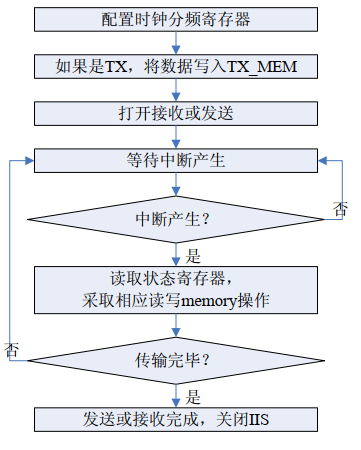
\includegraphics[width=0.5\linewidth]{./img/I2s/I2s_structure} 

}

\caption{I2S控制器操作流程图}\label{fig:I2S}
\end{figure}

如果需要用到DMA搬运则需要在使能I2s之前配置DMA并使能。

\hypertarget{ux6ce8ux610fux70b9-1}{%
\subsection{注意点}\label{ux6ce8ux610fux70b9-1}}

\begin{itemize}
\item
  I2s时钟源可以选择晶振24M时钟和PLL时钟,要注意是选择哪一个时钟源
\item
  I2s数据可能会进行采样,需要注意具体的数据结构以及对应的数据处理,如是否需要数据移位等
\item
  当前I2s支持的发送/接收数据位宽为16-32bit,需要查阅mic文档或其他使用手册来确定数据位宽,否则不能正常工作
\item
  配置DMA要在使能I2s之前完成,使能I2s一定是最后一步
\item
  建议采用DMA乒乓搬运的方式来传输I2s数据
\end{itemize}

\hypertarget{ux7f16ux7a0bux6307ux5357-1}{%
\section{编程指南}\label{ux7f16ux7a0bux6307ux5357-1}}

\hypertarget{ux9a71ux52a8ux63a5ux53e3-1}{%
\subsection{驱动接口}\label{ux9a71ux52a8ux63a5ux53e3-1}}

\begin{itemize}
\item
  I2S\_ConfigClk:I2s时钟配置接口
\item
  I2S\_Config:I2s配置接口
\item
  I2S\_ConfigIRQ:I2s中断配置接口
\item
  I2S\_DMAEnable:I2s DMA使能接口
\item
  I2S\_Enable:I2s使能接口
\item
  I2S\_PopRxFIFO、I2S\_PushTxFIFO:I2s FIFO读写接口
\item
  I2S\_ClearRxFIFO、I2S\_ClearTxFIFO:I2s清FIFO接口
\item
  I2S\_GetIntState、I2S\_ClearIntState:I2s获取中断、清中断接口
\item
  I2S\_GetRxFIFOCount、I2S\_GetTxFIFOCount:I2s获取FIFO数据数量接口
\item
  I2S\_DataFromPDM:I2s获取PDM数据接口
\end{itemize}

\hypertarget{ux4ee3ux7801ux793aux4f8b-1}{%
\subsection{代码示例}\label{ux4ee3ux7801ux793aux4f8b-1}}

下面将通过实际代码展示I2s的基本配置及使用代码。

\hypertarget{i2sux914dux7f6e}{%
\subsubsection{I2s配置}\label{i2sux914dux7f6e}}

\begin{Shaded}
\begin{Highlighting}[]
\PreprocessorTok{#define I2S_PIN_BCLK        28}
\PreprocessorTok{#define I2S_PIN_IN          29}
\PreprocessorTok{#define I2S_PIN_LRCLK       30}
\DataTypeTok{void}\NormalTok{ I2sSetup(}\DataTypeTok{void}\NormalTok{)}
\NormalTok{\{}
    \CommentTok{// pinctrl & GPIO mux}
\NormalTok{    PINCTRL_SetPadMux(I2S_PIN_BCLK, IO_SOURCE_I2S_BCLK_OUT);}
\NormalTok{    PINCTRL_SetPadMux(I2S_PIN_IN, IO_SOURCE_I2S_DATA_IN);}
\NormalTok{    PINCTRL_SelI2sIn(IO_NOT_A_PIN, IO_NOT_A_PIN, I2S_PIN_IN);}
\NormalTok{    PINCTRL_SetPadMux(I2S_PIN_LRCLK, IO_SOURCE_I2S_LRCLK_OUT);}
\NormalTok{    PINCTRL_Pull(IO_SOURCE_I2S_DATA_IN, PINCTRL_PULL_DOWN);}
    
    \CommentTok{// CLK & Register}
\NormalTok{    SYSCTRL_ConfigPLLClk(}\DecValTok{6}\NormalTok{, }\DecValTok{128}\NormalTok{, }\DecValTok{2}\NormalTok{); }\CommentTok{// sorce clk PLL = 256MHz}
\NormalTok{    SYSCTRL_SelectI2sClk(SYSCTRL_CLK_PLL_DIV_1 + }\DecValTok{4}\NormalTok{); }\CommentTok{// I2s_Clk = 51.2MHz}
\NormalTok{    I2S_ConfigClk(APB_I2S, }\DecValTok{25}\NormalTok{, }\DecValTok{32}\NormalTok{); }\CommentTok{// F_bclk = 1.024MHz, F_lrclk = 16K}
\NormalTok{    I2S_ConfigIRQ(APB_I2S, }\DecValTok{0}\NormalTok{, }\DecValTok{1}\NormalTok{, }\DecValTok{0}\NormalTok{, }\DecValTok{10}\NormalTok{);}
\NormalTok{    I2S_DMAEnable(APB_I2S, }\DecValTok{0}\NormalTok{, }\DecValTok{0}\NormalTok{);    }
\NormalTok{    I2S_Config(APB_I2S, I2S_ROLE_MASTER, I2S_MODE_STANDARD, }\DecValTok{0}\NormalTok{, }\DecValTok{0}\NormalTok{, }\DecValTok{0}\NormalTok{, }\DecValTok{1}\NormalTok{, }\DecValTok{24}\NormalTok{);}

    \CommentTok{// I2s interrupt}
\NormalTok{    platform_set_irq_callback(PLATFORM_CB_IRQ_I2S, cb_isr, }\DecValTok{0}\NormalTok{);}
\NormalTok{\}}
\end{Highlighting}
\end{Shaded}

\hypertarget{i2sux4f7fux80fd}{%
\subsubsection{I2s使能}\label{i2sux4f7fux80fd}}

I2s使能分3种情况:I2s发送、I2s接收、使用DMA搬运

接收:

\begin{Shaded}
\begin{Highlighting}[]
\DataTypeTok{void}\NormalTok{ I2sStart(}\DataTypeTok{void}\NormalTok{)}
\NormalTok{\{}
\NormalTok{    I2S_ClearRxFIFO(APB_I2S);}
\NormalTok{    I2S_Enable(APB_I2S, }\DecValTok{0}\NormalTok{, }\DecValTok{1}\NormalTok{);}
\NormalTok{\}}
\end{Highlighting}
\end{Shaded}

发送:

\begin{Shaded}
\begin{Highlighting}[]
\DataTypeTok{uint8_t}\NormalTok{  sendSize = }\DecValTok{10}\NormalTok{;}
\DataTypeTok{uint32_t}\NormalTok{ sendData[}\DecValTok{10}\NormalTok{];}
\DataTypeTok{void}\NormalTok{ I2sStart(}\DataTypeTok{void}\NormalTok{)}
\NormalTok{\{}
    \DataTypeTok{int}\NormalTok{ i; }
\NormalTok{    I2S_ClearTxFIFO(APB_I2S);}
    \CommentTok{// push data into TX_FIFO first}
    \ControlFlowTok{for}\NormalTok{ (i = }\DecValTok{0}\NormalTok{; i < sendSize; i++) \{}
\NormalTok{        I2S_PushTxFIFO(APB_I2S, sendData[i]);}
\NormalTok{    \}}
\NormalTok{    I2S_Enable(APB_I2S, }\DecValTok{0}\NormalTok{, }\DecValTok{1}\NormalTok{);}
\NormalTok{\}}
\end{Highlighting}
\end{Shaded}

使用DMA(接收):

\begin{Shaded}
\begin{Highlighting}[]
\PreprocessorTok{#define CHANNEL_ID  0}
\NormalTok{DMA_Descriptor test __attribute__((aligned (}\DecValTok{8}\NormalTok{)));                                }
\DataTypeTok{void}\NormalTok{ I2sStart(}\DataTypeTok{uint32_t}\NormalTok{ data)}
\NormalTok{\{}
\NormalTok{   DMA_EnableChannel(CHANNEL_ID, &test);}
\NormalTok{   I2S_ClearRxFIFO(APB_I2S);}
\NormalTok{   I2S_DMAEnable(APB_I2S, }\DecValTok{1}\NormalTok{, }\DecValTok{1}\NormalTok{);    }
\NormalTok{   I2S_Enable(APB_I2S, }\DecValTok{0}\NormalTok{, }\DecValTok{1}\NormalTok{);}
\NormalTok{\}}
\end{Highlighting}
\end{Shaded}

无论哪种情况都必须最后一步使能I2s,否则I2s工作异常。

\hypertarget{i2sux4e2dux65ad}{%
\subsubsection{I2s中断}\label{i2sux4e2dux65ad}}

接收:

\begin{Shaded}
\begin{Highlighting}[]
\DataTypeTok{uint32_t}\NormalTok{ cb_isr(}\DataTypeTok{void}\NormalTok{ *user_data)}
\NormalTok{\{ }
    \DataTypeTok{uint32_t}\NormalTok{ state = I2S_GetIntState(APB_I2S);}
\NormalTok{    I2S_ClearIntState(APB_I2S, state);}

    \DataTypeTok{int}\NormalTok{ i = I2S_GetRxFIFOCount(APB_I2S);}

    \ControlFlowTok{while}\NormalTok{ (i) \{}
        \DataTypeTok{uint32_t}\NormalTok{ data = I2S_PopRxFIFO(APB_I2S);}
\NormalTok{        i--;}
        \CommentTok{// do something with data}
\NormalTok{    \}}

    \ControlFlowTok{return} \DecValTok{0}\NormalTok{;}
\NormalTok{\}}
\end{Highlighting}
\end{Shaded}

发送:

\begin{Shaded}
\begin{Highlighting}[]
\DataTypeTok{uint8_t}\NormalTok{  sendSize = }\DecValTok{10}\NormalTok{;}
\DataTypeTok{uint32_t}\NormalTok{ sendData[}\DecValTok{10}\NormalTok{];}
\DataTypeTok{uint32_t}\NormalTok{ cb_isr(}\DataTypeTok{void}\NormalTok{ *user_data)}
\NormalTok{\{ }
    \DataTypeTok{uint32_t}\NormalTok{ state = I2S_GetIntState(APB_I2S);}
\NormalTok{    I2S_ClearIntState(APB_I2S, state);}

    \DataTypeTok{int}\NormalTok{ i;}
    \ControlFlowTok{for}\NormalTok{ (i = }\DecValTok{0}\NormalTok{; i < sendSize; i++) \{}
\NormalTok{        I2S_PushTxFIFO(APB_I2S, sendData[i]);}
\NormalTok{    \}}
    \ControlFlowTok{return} \DecValTok{0}\NormalTok{;}
\NormalTok{\}}
\end{Highlighting}
\end{Shaded}

\hypertarget{i2s-ux4e52ux4e53dma}{%
\subsubsection{I2s \& 乒乓DMA}\label{i2s-ux4e52ux4e53dma}}

下面以经典的DMA乒乓搬运I2s接收数据为例展示I2s实际使用方法。

这里我们采用16K采样率,单个数据帧固定64位,和DMA协商握手、burstSize=8、一次搬运80个数据。

\begin{Shaded}
\begin{Highlighting}[]
\PreprocessorTok{#define I2S_PIN_BCLK        28}
\PreprocessorTok{#define I2S_PIN_IN          29}
\PreprocessorTok{#define I2S_PIN_LRCLK       30}
\PreprocessorTok{#define CHANNEL_ID  0}
\DataTypeTok{uint32_t}\NormalTok{ pingpang_buff[}\DecValTok{2}\NormalTok{][}\DecValTok{80}\NormalTok{];}
\NormalTok{DMA_Descriptor test[}\DecValTok{2}\NormalTok{] __attribute__((aligned (}\DecValTok{8}\NormalTok{)));}
\DataTypeTok{uint8_t}\NormalTok{ pingpang = }\DecValTok{0}\NormalTok{;}
\DataTypeTok{static} \DataTypeTok{uint32_t}\NormalTok{ DMA_cb_isr(}\DataTypeTok{void}\NormalTok{ *user_data)}
\NormalTok{\{ }
      \DataTypeTok{uint32_t}\NormalTok{ state = DMA_GetChannelIntState(CHANNEL_ID);}
\NormalTok{      DMA_ClearChannelIntState(CHANNEL_ID, state);}

\NormalTok{      pingpang ^= }\DecValTok{1}\NormalTok{;}
\NormalTok{    DMA_EnableChannel(CHANNEL_ID, &test[pingpang]);}
    \DataTypeTok{uint32_t}\NormalTok{ *data = (pingpang) ? (pingpang_buff[}\DecValTok{0}\NormalTok{]) : (pingpang_buff[}\DecValTok{1}\NormalTok{]);}

    \CommentTok{// do something with data-buffer's data}
    
    \ControlFlowTok{return} \DecValTok{0}\NormalTok{;}
\NormalTok{\}}

\DataTypeTok{void}\NormalTok{ DMA_SetUpPingPang(}\DataTypeTok{void}\NormalTok{)}
\NormalTok{\{}
\NormalTok{    DMA_Reset();}
\NormalTok{    platform_set_irq_callback(PLATFORM_CB_IRQ_DMA, DMA_cb_isr, }\DecValTok{0}\NormalTok{);  }
\NormalTok{    test[}\DecValTok{0}\NormalTok{].Next = &test[}\DecValTok{1}\NormalTok{];}
\NormalTok{    test[}\DecValTok{1}\NormalTok{].Next = &test[}\DecValTok{0}\NormalTok{];    }\CommentTok{// make a DMA link cycle}
\NormalTok{    DMA_PreparePeripheral2RAM(&test[}\DecValTok{0}\NormalTok{], }
\NormalTok{                              pingpang_buff[}\DecValTok{0}\NormalTok{], }
\NormalTok{                              SYSCTRL_DMA_I2S_RX, }
                              \DecValTok{80}\NormalTok{, }
\NormalTok{                              DMA_ADDRESS_INC, }
                              \DecValTok{0}\NormalTok{ | }\DecValTok{8}\NormalTok{ << }\DecValTok{24}\NormalTok{ | }\DecValTok{1}\NormalTok{ << }\DecValTok{28}\NormalTok{);}
\NormalTok{    DMA_PreparePeripheral2RAM(&test[}\DecValTok{1}\NormalTok{], }
\NormalTok{                              pingpang_buff[}\DecValTok{1}\NormalTok{], }
\NormalTok{                              SYSCTRL_DMA_I2S_RX, }
                              \DecValTok{80}\NormalTok{, }
\NormalTok{                              DMA_ADDRESS_INC, }
                              \DecValTok{0}\NormalTok{ | }\DecValTok{8}\NormalTok{ << }\DecValTok{24}\NormalTok{ | }\DecValTok{1}\NormalTok{ << }\DecValTok{28}\NormalTok{);}
\NormalTok{    DMA_EnableChannel(CHANNEL_ID, &test[pingpang]);}
\NormalTok{\}}
\DataTypeTok{void}\NormalTok{ I2sSetup(}\DataTypeTok{void}\NormalTok{)}
\NormalTok{\{}
    \CommentTok{// pinctrl & GPIO mux}
\NormalTok{    PINCTRL_SetPadMux(I2S_PIN_BCLK, IO_SOURCE_I2S_BCLK_OUT);}
\NormalTok{    PINCTRL_SetPadMux(I2S_PIN_IN, IO_SOURCE_I2S_DATA_IN);}
\NormalTok{    PINCTRL_SelI2sIn(IO_NOT_A_PIN, IO_NOT_A_PIN, I2S_PIN_IN);}
\NormalTok{    PINCTRL_SetPadMux(I2S_PIN_LRCLK, IO_SOURCE_I2S_LRCLK_OUT);}
\NormalTok{    PINCTRL_Pull(IO_SOURCE_I2S_DATA_IN, PINCTRL_PULL_DOWN);}
    
    \CommentTok{// CLK & Register}
\NormalTok{    SYSCTRL_ConfigPLLClk(}\DecValTok{6}\NormalTok{, }\DecValTok{128}\NormalTok{, }\DecValTok{2}\NormalTok{); }\CommentTok{// sorce clk PLL = 256MHz}
\NormalTok{    SYSCTRL_SelectI2sClk(SYSCTRL_CLK_PLL_DIV_1 + }\DecValTok{4}\NormalTok{); }\CommentTok{// I2s_Clk = 51.2MHz}
\NormalTok{    I2S_ConfigClk(APB_I2S, }\DecValTok{25}\NormalTok{, }\DecValTok{32}\NormalTok{); }\CommentTok{// F_bclk = 1.024MHz, F_lrclk = 16K}
\NormalTok{    I2S_ConfigIRQ(APB_I2S, }\DecValTok{0}\NormalTok{, }\DecValTok{1}\NormalTok{, }\DecValTok{0}\NormalTok{, }\DecValTok{8}\NormalTok{);}
\NormalTok{    I2S_DMAEnable(APB_I2S, }\DecValTok{0}\NormalTok{, }\DecValTok{0}\NormalTok{);    }
\NormalTok{    I2S_Config(APB_I2S, I2S_ROLE_MASTER, I2S_MODE_STANDARD, }\DecValTok{0}\NormalTok{, }\DecValTok{0}\NormalTok{, }\DecValTok{0}\NormalTok{, }\DecValTok{1}\NormalTok{, }\DecValTok{24}\NormalTok{);}

    \CommentTok{// setup pingpang DMA}
\NormalTok{    DMA_SetUpPingPang();}
    
    \CommentTok{// start working}
\NormalTok{    I2S_ClearRxFIFO(APB_I2S);}
\NormalTok{    I2S_DMAEnable(APB_I2S, }\DecValTok{1}\NormalTok{, }\DecValTok{1}\NormalTok{);    }
\NormalTok{    I2S_Enable(APB_I2S, }\DecValTok{0}\NormalTok{, }\DecValTok{1}\NormalTok{);}
\NormalTok{\}}
\end{Highlighting}
\end{Shaded}

DMA的具体用法请参见本手册DMA一节。

更加系统化的I2s代码请参考SDK中voice\_remote\_ctrl例程。

\hypertarget{ir-ux7ea2ux5916}{%
\chapter{IR 红外}\label{ir-ux7ea2ux5916}}

\hypertarget{ux529fux80fdux6982ux8ff0-2}{%
\section{功能概述}\label{ux529fux80fdux6982ux8ff0-2}}

\begin{itemize}
\tightlist
\item
  支持红外发射\&接收
\item
  时序可调整,支持多种编码
\end{itemize}

\hypertarget{ux4f7fux7528ux8bf4ux660e-2}{%
\section{使用说明}\label{ux4f7fux7528ux8bf4ux660e-2}}

\hypertarget{ux53c2ux6570ux4e0dux540cux7f16ux7801ux7684ux65f6ux95f4ux53c2ux6570}{%
\subsection{参数(不同编码的时间参数)}\label{ux53c2ux6570ux4e0dux540cux7f16ux7801ux7684ux65f6ux95f4ux53c2ux6570}}

\begin{Shaded}
\begin{Highlighting}[]
\CommentTok{//32KHz 调制时钟}
\PreprocessorTok{#define FCLK            32000}

\CommentTok{//NEC 载波频率38KHz}
\PreprocessorTok{#define NEC_WAVE_FREQ   38000}

\CommentTok{// RC5 载波频率36KHz}
\PreprocessorTok{#define RC5_WAVE_FREQ   36000}

\CommentTok{// 计算载波频率发生器数据,由此产生如38KHz NEC的载波,NEC与TC9012通用38KHz载波}
\PreprocessorTok{#define IR_WAVE_NEC_TC9012_FREQ (OSC_CLK_FREQ/NEC_WAVE_FREQ)    }
\PreprocessorTok{#define IR_WAVE_RC5_FREQ (OSC_CLK_FREQ/RC5_WAVE_FREQ)  }

\CommentTok{//通过FCLK产生各种协议每bit位调制周期最小单位,如NEC协议中,560us为最小调制周期,NEC:bit 0:560us载波+560us不载波,bit 1:560 us载波+560*3 us不载波}
\PreprocessorTok{#define NEC_UINT    (FCLK*560/1000000+1)}
\PreprocessorTok{#define TC9012_UINT (FCLK*260/1000000+1)}
\PreprocessorTok{#define RC5_UINT    (FCLK*889/1000000+1)}

\CommentTok{//不必要的参数}
\PreprocessorTok{#define INESSENTIAL     0}

\KeywordTok{typedef} \KeywordTok{struct}
\NormalTok{\{}
    \DataTypeTok{uint16_t}\NormalTok{ timer1;}\CommentTok{//发送模式下,表示引导码低电平时间:如NEC为16*UNIT = 9ms,接收模式下与timer2组成检测引导码低电平窗口}
    \DataTypeTok{uint16_t}\NormalTok{ timer2;}\CommentTok{//发送模式下,表示重复码低电平时间:如NEC为4*UNIT = 2.25ms,接收模式下与timer1组成检测引导码低窗口}
    \DataTypeTok{uint16_t}\NormalTok{ timer3;}\CommentTok{//发送模式下,表示引导码高电平时间:如NEC为8*UNIT = 4.5ms,接收模式下与timer4组成检测引导码高电平+低电平窗口}
    \DataTypeTok{uint16_t}\NormalTok{ timer4;}\CommentTok{//发送模式下,表示重复码高电平时间:如NEC为UNIT = 560us,接收模式下与timer3组成检测引导码高电平+低电平窗口}
    \DataTypeTok{uint16_t}\NormalTok{ timer5;}\CommentTok{//接收时接收超时定时器,发射不必关注}
    \DataTypeTok{uint16_t}\NormalTok{ btimer1;}\CommentTok{//逻辑 0 的bit时长:如NEC = 2*UINT = 1.12ms.}
    \DataTypeTok{uint16_t}\NormalTok{ btimer2;}\CommentTok{//逻辑 1 的bit时长:如NEC = 4*UINT = 2.25ms.}
    \DataTypeTok{uint16_t}\NormalTok{ bit_cycle;}\CommentTok{//发射模式下:bit调制周期最小单位,如NEC为560us,接收模式下为bit检测超时时间}
    \DataTypeTok{uint16_t}\NormalTok{ carry_low;}\CommentTok{//载波低电平时长,与carry_high组合形成占空比可调的载波波形,如NEC为38KHz 30%占空比载波则carry_low = 2/3*载波周期,carry_high = 1/3*载波周期}
    \DataTypeTok{uint16_t}\NormalTok{ carry_high;}\CommentTok{//载波高电平时长,与carry_low组合形成占空比可调的载波波形,如NEC为38KHz 30%占空比载波则carry_low = 2/3*载波周期,carry_high = 1/3*载波周期}
\NormalTok{\}Ir_mode_param_t;}

\CommentTok{//由于发送和接收初始化不同参数 定义结构体表示接收发送初始化参数。}
\KeywordTok{typedef} \KeywordTok{struct}\NormalTok{\{}
\NormalTok{    Ir_mode_param_t param_tx;}
\NormalTok{    Ir_mode_param_t param_rx;}
\NormalTok{\}Ir_type_param_t;}

\CommentTok{//定义初始化数据,初始化函数体根据不同协议自动从此表适配参数}
\DataTypeTok{const} \DataTypeTok{static}\NormalTok{ Ir_type_param_t t_ir_type_param_table[] = }
\NormalTok{\{}
\NormalTok{    \{}\CommentTok{//NEC param}
\NormalTok{        \{  }\CommentTok{//TX}
            \DecValTok{16}\NormalTok{*NEC_UINT-}\DecValTok{1}\NormalTok{,}\DecValTok{4}\NormalTok{*NEC_UINT-}\DecValTok{1}\NormalTok{,}\DecValTok{8}\NormalTok{*NEC_UINT-}\DecValTok{1}\NormalTok{,}\DecValTok{1}\NormalTok{*NEC_UINT-}\DecValTok{1}\NormalTok{,INESSENTIAL,}
            \DecValTok{2}\NormalTok{*NEC_UINT-}\DecValTok{1}\NormalTok{, }\DecValTok{4}\NormalTok{*NEC_UINT-}\DecValTok{1}\NormalTok{,}\DecValTok{1}\NormalTok{*NEC_UINT-}\DecValTok{1}\NormalTok{,IR_WAVE_NEC_TC9012_FREQ*}\DecValTok{2}\NormalTok{/}\DecValTok{3}\NormalTok{,IR_WAVE_NEC_TC9012_FREQ*}\DecValTok{1}\NormalTok{/}\DecValTok{3}\NormalTok{\},}
\NormalTok{        \{   }\CommentTok{//RX}
            \DecValTok{14}\NormalTok{*NEC_UINT-}\DecValTok{1}\NormalTok{,}\DecValTok{18}\NormalTok{*NEC_UINT-}\DecValTok{1}\NormalTok{,}\DecValTok{22}\NormalTok{*NEC_UINT-}\DecValTok{1}\NormalTok{,}\DecValTok{26}\NormalTok{*NEC_UINT-}\DecValTok{1}\NormalTok{,}\BaseNTok{0xfff}\NormalTok{,}
\NormalTok{            INESSENTIAL,}\DecValTok{2}\NormalTok{*NEC_UINT-}\DecValTok{1}\NormalTok{,}\BaseNTok{0x7f}\NormalTok{,INESSENTIAL,INESSENTIAL\},    }
\NormalTok{    \},}
\NormalTok{    \{}\CommentTok{//TC9012 param}
\NormalTok{        \{   }\CommentTok{//TX}
            \DecValTok{16}\NormalTok{*TC9012_UINT-}\DecValTok{1}\NormalTok{,}\DecValTok{8}\NormalTok{*TC9012_UINT-}\DecValTok{1}\NormalTok{,}\DecValTok{16}\NormalTok{*TC9012_UINT-}\DecValTok{1}\NormalTok{,}\DecValTok{2}\NormalTok{*TC9012_UINT-}\DecValTok{1}\NormalTok{,INESSENTIAL,}
            \DecValTok{4}\NormalTok{*TC9012_UINT-}\DecValTok{1}\NormalTok{,}\DecValTok{6}\NormalTok{*TC9012_UINT-}\DecValTok{1}\NormalTok{,}\DecValTok{2}\NormalTok{*TC9012_UINT-}\DecValTok{1}\NormalTok{,IR_WAVE_NEC_TC9012_FREQ*}\DecValTok{2}\NormalTok{/}\DecValTok{3}\NormalTok{,IR_WAVE_NEC_TC9012_FREQ*}\DecValTok{1}\NormalTok{/}\DecValTok{3}\NormalTok{\},}
\NormalTok{        \{    }\CommentTok{//RX}
            \DecValTok{28}\NormalTok{*TC9012_UINT-}\DecValTok{1}\NormalTok{,}\DecValTok{36}\NormalTok{*TC9012_UINT-}\DecValTok{1}\NormalTok{,}\DecValTok{44}\NormalTok{*TC9012_UINT-}\DecValTok{1}\NormalTok{,}\DecValTok{32}\NormalTok{*TC9012_UINT-}\DecValTok{1}\NormalTok{,}\BaseNTok{0xfff}\NormalTok{,INESSENTIAL,}
            \DecValTok{4}\NormalTok{*TC9012_UINT-}\DecValTok{1}\NormalTok{,}\BaseNTok{0x7f}\NormalTok{,INESSENTIAL,INESSENTIAL\},    }
\NormalTok{    \},    }
\NormalTok{    \{}\CommentTok{//RC5 param}
\NormalTok{        \{   }\CommentTok{//TX}
            \DecValTok{2}\NormalTok{*RC5_UINT-}\DecValTok{1}\NormalTok{,}\DecValTok{2}\NormalTok{*RC5_UINT-}\DecValTok{1}\NormalTok{,INESSENTIAL,INESSENTIAL,INESSENTIAL,}\DecValTok{2}\NormalTok{*RC5_UINT-}\DecValTok{1}\NormalTok{,}
\NormalTok{            INESSENTIAL,}\DecValTok{1}\NormalTok{*RC5_UINT,IR_WAVE_RC5_FREQ*}\DecValTok{2}\NormalTok{/}\DecValTok{3}\NormalTok{,IR_WAVE_RC5_FREQ*}\DecValTok{1}\NormalTok{/}\DecValTok{3}\NormalTok{\},}
        
\NormalTok{        \{   }\CommentTok{//RX}
            \DecValTok{1}\NormalTok{*RC5_UINT-}\DecValTok{2}\NormalTok{,}\DecValTok{1}\NormalTok{*RC5_UINT,}\DecValTok{3}\NormalTok{*RC5_UINT-}\DecValTok{1}\NormalTok{,}\DecValTok{5}\NormalTok{*RC5_UINT-}\DecValTok{1}\NormalTok{,INESSENTIAL,}\DecValTok{1}\NormalTok{*RC5_UINT-}\DecValTok{3}\NormalTok{,}
            \DecValTok{1}\NormalTok{*RC5_UINT-}\DecValTok{1}\NormalTok{,}\DecValTok{2}\NormalTok{*RC5_UINT-}\DecValTok{1}\NormalTok{,INESSENTIAL,INESSENTIAL\},    }
\NormalTok{    \}}
\NormalTok{\};}
\end{Highlighting}
\end{Shaded}

\hypertarget{ux7ea2ux5916ux53d1ux5c04ux63a5ux6536}{%
\subsection{红外发射接收}\label{ux7ea2ux5916ux53d1ux5c04ux63a5ux6536}}

\hypertarget{ux914dux7f6epin-8}{%
\subsubsection{配置pin}\label{ux914dux7f6epin-8}}

\begin{Shaded}
\begin{Highlighting}[]
\PreprocessorTok{#define IR_PIN GIO_GPIO_17}
\DataTypeTok{void}\NormalTok{ setup_peripherals_ir_module(}\DataTypeTok{void}\NormalTok{)}
\NormalTok{\{}
    \CommentTok{// 打开时钟}
    \CommentTok{// 大于等于GPIO 18则使用SYSCTRL_ClkGate_APB_GPIO1, 否则是SYSCTRL_ClkGate_APB_GPIO0}
\NormalTok{    SYSCTRL_ClearClkGateMulti(   (}\DecValTok{1}\NormalTok{ << SYSCTRL_ClkGate_APB_GPIO0)}
\NormalTok{                                | (}\DecValTok{1}\NormalTok{ << SYSCTRL_ClkGate_APB_GPIO1)}
\NormalTok{                                | (}\DecValTok{1}\NormalTok{ << SYSCTRL_ITEM_APB_IR)}
\NormalTok{                                | (}\DecValTok{1}\NormalTok{ << SYSCTRL_ClkGate_APB_PinCtrl));}
                                
\NormalTok{    PINCTRL_SetPadMux(IR_PIN,IO_SOURCE_IR_DATA_OUT);}
\NormalTok{    platform_set_irq_callback(PLATFORM_CB_IRQ_IR_INT, IRQHandler_IR_INT, NULL);}
\NormalTok{\}}
\end{Highlighting}
\end{Shaded}

\hypertarget{ux914dux7f6eux6a21ux5757}{%
\subsubsection{配置模块}\label{ux914dux7f6eux6a21ux5757}}

\begin{Shaded}
\begin{Highlighting}[]
\DataTypeTok{static} \DataTypeTok{void}\NormalTok{ user_ir_device_init(IR_IrMode_e mode,IR_TxRxMode_e tx_rx_mode,GIO_Index_t irpin)}
\NormalTok{\{}
\NormalTok{    IR_CtrlSetIrMode(APB_IR,mode);}
\NormalTok{    IR_CtrlSetTxRxMode(APB_IR,tx_rx_mode);}
\NormalTok{    IR_CtrlSetIrIntEn(APB_IR);}
    
    \ControlFlowTok{if}\NormalTok{(IR_TXRX_MODE_TX_MODE == tx_rx_mode)}
\NormalTok{    \{}
\NormalTok{        IR_TxConfigIrTxPol(APB_IR);}
\NormalTok{        IR_TxConfigCarrierCntClr(APB_IR);}
\NormalTok{        IR_TxConfigIrIntEn(APB_IR);}
\NormalTok{        IR_CarryConfigSetIrCarryLow(APB_IR,t_ir_type_param_table[mode].param_tx.carry_low);   }\CommentTok{//30% pwm}
\NormalTok{        IR_CarryConfigSetIrCarryHigh(APB_IR,t_ir_type_param_table[mode].param_tx.carry_high);}
\NormalTok{        IR_TimeSetIrTime1(APB_IR,t_ir_type_param_table[mode].param_tx.timer1);}
\NormalTok{        IR_TimeSetIrTime2(APB_IR,t_ir_type_param_table[mode].param_tx.timer2);}
\NormalTok{        IR_TimeSetIrTime3(APB_IR,t_ir_type_param_table[mode].param_tx.timer3 );}
\NormalTok{        IR_TimeSetIrTime4(APB_IR,t_ir_type_param_table[mode].param_tx.timer4); }
\NormalTok{        IR_CtrlIrSetBitTime1(APB_IR,t_ir_type_param_table[mode].param_tx.btimer1);}
\NormalTok{        IR_CtrlIrSetBitTime2(APB_IR,t_ir_type_param_table[mode].param_tx.btimer2);    }
\NormalTok{        IR_CtrlIrSetIrBitCycle(APB_IR,t_ir_type_param_table[mode].param_tx.bit_cycle);        }
\NormalTok{        PINCTRL_SetPadMux(irpin,IO_SOURCE_IR_DATA_OUT);}
\NormalTok{    \}}
    \ControlFlowTok{else}\NormalTok{\{}
\NormalTok{        IR_CtrlSetIrEndDetectEn(APB_IR);}\CommentTok{//end code detect en}
\NormalTok{        IR_CtrlSetIrIntVerifyEn(APB_IR);}
\NormalTok{        IR_CtrlIrUsercodeVerify(APB_IR);}
\NormalTok{        IR_CtrlIrDatacodeVerify(APB_IR);}
\NormalTok{        IR_TimeSetIrTime1(APB_IR,t_ir_type_param_table[mode].param_rx.timer1);}
\NormalTok{        IR_TimeSetIrTime2(APB_IR,t_ir_type_param_table[mode].param_rx.timer2);}
\NormalTok{        IR_TimeSetIrTime3(APB_IR,t_ir_type_param_table[mode].param_rx.timer3);}
\NormalTok{        IR_TimeSetIrTime4(APB_IR,t_ir_type_param_table[mode].param_rx.timer4); }
\NormalTok{        IR_TimeSetIrTime5(APB_IR,t_ir_type_param_table[mode].param_rx.timer5); }
\NormalTok{        IR_CtrlIrSetBitTime1(APB_IR,t_ir_type_param_table[mode].param_rx.btimer1);}
\NormalTok{        IR_CtrlIrSetBitTime2(APB_IR,t_ir_type_param_table[mode].param_rx.btimer2);    }
\NormalTok{        IR_CtrlIrSetIrBitCycle(APB_IR,t_ir_type_param_table[mode].param_rx.bit_cycle);   }
\NormalTok{        PINCTRL_SetPadMux(irpin,IO_SOURCE_IR_DATA_IN);}
\NormalTok{    \}}
\NormalTok{    IR_CtrlEnable(APB_IR);}
\NormalTok{\}}
\end{Highlighting}
\end{Shaded}

\hypertarget{ir-ux4e2dux65ad}{%
\subsubsection{IR 中断}\label{ir-ux4e2dux65ad}}

\begin{Shaded}
\begin{Highlighting}[]
\DataTypeTok{static} \DataTypeTok{uint32_t}\NormalTok{ IRQHandler_IR_INT(}\DataTypeTok{void}\NormalTok{ *user_data)}
\NormalTok{\{}
    \ControlFlowTok{if}\NormalTok{(IR_FsmGetIrTransmitOk(APB_IR))}
\NormalTok{        ;}\CommentTok{//platform_printf("int ir send ok\textbackslash{}n");}
    \ControlFlowTok{if}\NormalTok{(IR_FsmGetIrTxRepeat(APB_IR))}
\NormalTok{        ;}\CommentTok{//platform_printf("int ir repeat ok\textbackslash{}n");}
    \ControlFlowTok{return} \DecValTok{0}\NormalTok{;}
\NormalTok{\}}
\end{Highlighting}
\end{Shaded}

\begin{center}\rule{0.5\linewidth}{0.5pt}\end{center}

\hypertarget{ch-PDM}{%
\chapter{PDM简介}\label{ch-PDM}}

PDM全称pulse density modulation,即脉冲密度调制。

PDM模块处理来自外部音频前端(如数字麦克风)的脉冲密度调制信号的输入。该模块生成PDM时钟,支持双通道数据输入。

\hypertarget{ux529fux80fdux63cfux8ff0-2}{%
\section{功能描述}\label{ux529fux80fdux63cfux8ff0-2}}

\hypertarget{ux7279ux70b9-2}{%
\subsection{特点}\label{ux7279ux70b9-2}}

\begin{itemize}
\item
  支持双通道,数据输入相同
\item
  16kHz输出采样率,24位采样
\item
  HW抽取过滤器
\item
  时钟和输出采样率之间的可选比为64或80
\item
  支持DMA和I2S的样本缓冲
\end{itemize}

\hypertarget{pdm-pcm}{%
\subsection{PDM \& PCM}\label{pdm-pcm}}

PDM和PCM同为用数字信号表示模拟信号的音频数据调制方法,其主要区别是:

\begin{itemize}
\item
  PDM不像PCM等间隔采样
\item
  PDM只有1位非0即1的输出,而PCM采样结果可以是Nbit
\item
  PDM使用远高于PCM采样率的时钟频率进行采样
\item
  PDM逻辑相对PCM复杂
\item
  PDM只需要2根信号线,即时钟线和数据线;PCM需要4根线
\end{itemize}

\hypertarget{ux4f7fux7528ux65b9ux6cd5-2}{%
\section{使用方法}\label{ux4f7fux7528ux65b9ux6cd5-2}}

\hypertarget{ux65b9ux6cd5ux6982ux8ff0-2}{%
\subsection{方法概述}\label{ux65b9ux6cd5ux6982ux8ff0-2}}

PDM使用方法分为PDM结合I2s使用和PDM数据直接DMA搬运两种。

PDM结合I2s:

\textbf{1.} PDM引脚GPIO配置(时钟、数据)

\textbf{2.} 外部时钟配置,使其处于工作模式

\textbf{3.} 写相应配置寄存器

\textbf{4.} 配置I2s数据源为PDM,配置I2s时钟、寄存器、中断

\textbf{5.} 使能PDM,使能I2s

\textbf{6.} 等待I2s中断产生

\textbf{7.} 读取状态寄存器,读取RX\_MEM中数据

\textbf{8.} 传输完毕,关闭PDM和I2S

PDM数据DMA搬运:

\textbf{1.} PDM引脚GPIO配置(时钟、数据)

\textbf{2.} 外部时钟配置,使其处于工作模式

\textbf{3.} 写相应配置寄存器

\textbf{4.} 配置DMA寄存器、中断

\textbf{5.} 使能DMA,使能PDM

\textbf{6.} 等待DMA中断产生

\textbf{7.} 传输完毕,关闭PDM和DMA

其中I2s和DMA相关配置不在本节介绍内容范围内,可参考本手册对应章节。

\hypertarget{ux6ce8ux610fux70b9-2}{%
\subsection{注意点}\label{ux6ce8ux610fux70b9-2}}

\begin{itemize}
\item
  I2s时钟源可以选择晶振24M时钟和PLL时钟,要注意是选择哪一个时钟源
\item
  建议选择晶振24M作为时钟源,这样可以获得较好的准确度和防抖动效果
\item
  需要查阅数字麦克风数据手册了解其时钟要求,并正确配置PDM时钟频率
\item
  结合I2s使用时要先使能PDM最后开启I2s
\item
  结合DMA使用时要先使能DMA最后开启PDM
\item
  建议采用DMA乒乓搬运的方式
\end{itemize}

\hypertarget{ux7f16ux7a0bux6307ux5357-2}{%
\section{编程指南}\label{ux7f16ux7a0bux6307ux5357-2}}

\hypertarget{ux9a71ux52a8ux63a5ux53e3-2}{%
\subsection{驱动接口}\label{ux9a71ux52a8ux63a5ux53e3-2}}

\begin{itemize}
\item
  PDM\_Config:PDM配置接口
\item
  PDM\_Start:PDM使能接口
\item
  PDM\_DmaEnable:PDM使能DMA接口
\end{itemize}

\hypertarget{ux4ee3ux7801ux793aux4f8b-2}{%
\subsection{代码示例}\label{ux4ee3ux7801ux793aux4f8b-2}}

下面以PDM结合I2s使用和PDM数据直接DMA搬运两种方式来展示PDM的具体使用方法。

已知现有mic使用的时钟频率为3M,I2s采样率16K。

\hypertarget{pdmux7ed3ux5408i2s}{%
\subsubsection{PDM结合I2s:}\label{pdmux7ed3ux5408i2s}}

\begin{Shaded}
\begin{Highlighting}[]
\PreprocessorTok{#define PDM_PIN_MCLK        28}
\PreprocessorTok{#define PDM_PIN_IN          29}
\DataTypeTok{static} \DataTypeTok{uint32_t}\NormalTok{ I2s_isr(}\DataTypeTok{void}\NormalTok{ *user_data)}
\NormalTok{\{ }
    \DataTypeTok{uint32_t}\NormalTok{ state = I2S_GetIntState(APB_I2S);}
\NormalTok{    I2S_ClearIntState(APB_I2S, state);}

    \DataTypeTok{int}\NormalTok{ i = I2S_GetRxFIFOCount(APB_I2S);}
    \ControlFlowTok{while}\NormalTok{ (i) \{}
        \CommentTok{// do something with these data}
\NormalTok{        i--;}
\NormalTok{    \}}
\NormalTok{\}}

\DataTypeTok{void}\NormalTok{ audio_input_setup(}\DataTypeTok{void}\NormalTok{)}
\NormalTok{\{}
    \CommentTok{// GPIO & Pin Ctrl}
\NormalTok{    PINCTRL_SetPadMux(PDM_PIN_MCLK, IO_SOURCE_PDM_DMIC_MCLK);}
\NormalTok{    PINCTRL_SetPadMux(PDM_PIN_IN, IO_SOURCE_PDM_DMIC_IN);}
\NormalTok{    PINCTRL_SelPdmIn(PDM_PIN_IN);}

    \CommentTok{// PDM clock configuration, 3M}
\NormalTok{    SYSCTRL_SetPdmClkDiv(}\DecValTok{8}\NormalTok{, }\DecValTok{1}\NormalTok{);}
\NormalTok{    SYSCTRL_SelectTypeAClk(SYSCTRL_ITEM_APB_PDM, SYSCTRL_CLK_ADC_DIV);}
    
    \CommentTok{// PDM register configuration}
\NormalTok{    PDM_Config(APB_PDM, }\DecValTok{0}\NormalTok{, }\DecValTok{1}\NormalTok{, }\DecValTok{1}\NormalTok{, }\DecValTok{1}\NormalTok{, }\DecValTok{0}\NormalTok{);    }

    \CommentTok{// I2s configuration, bclk=2.4M, samplerate=16K, data from PDM}
\NormalTok{    I2S_DataFromPDM(}\DecValTok{1}\NormalTok{);    }
\NormalTok{    I2S_ConfigClk(APB_I2S, }\DecValTok{5}\NormalTok{, }\DecValTok{75}\NormalTok{);}
\NormalTok{    I2S_ConfigIRQ(APB_I2S, }\DecValTok{0}\NormalTok{, }\DecValTok{1}\NormalTok{, }\DecValTok{0}\NormalTok{, }\DecValTok{10}\NormalTok{);}
\NormalTok{    I2S_DMAEnable(APB_I2S, }\DecValTok{0}\NormalTok{, }\DecValTok{0}\NormalTok{);    }
\NormalTok{    I2S_Config(APB_I2S, I2S_ROLE_MASTER, I2S_MODE_STANDARD, }\DecValTok{0}\NormalTok{, }\DecValTok{1}\NormalTok{, }\DecValTok{0}\NormalTok{, }\DecValTok{1}\NormalTok{, }\DecValTok{24}\NormalTok{);}
    
    \CommentTok{// I2s interruption}
\NormalTok{    platform_set_irq_callback(PLATFORM_CB_IRQ_I2S, I2s_isr, }\DecValTok{0}\NormalTok{);}

    \CommentTok{// enable I2s and PDM}
\NormalTok{    I2S_ClearRxFIFO(APB_I2S);}
\NormalTok{    PDM_Start(APB_PDM, }\DecValTok{1}\NormalTok{);}
\NormalTok{    I2S_Enable(APB_I2S, }\DecValTok{0}\NormalTok{, }\DecValTok{1}\NormalTok{);}
\NormalTok{\}}
\end{Highlighting}
\end{Shaded}

上面示例涉及到的关于I2s配置参考手册的I2s章节:

\hypertarget{pdmux6570ux636edmaux642cux8fd0}{%
\subsubsection{PDM数据DMA搬运}\label{pdmux6570ux636edmaux642cux8fd0}}

\begin{Shaded}
\begin{Highlighting}[]
\PreprocessorTok{#define PDM_PIN_MCLK        28}
\PreprocessorTok{#define PDM_PIN_IN          29}
\PreprocessorTok{#define CHANNEL_ID  0}
\DataTypeTok{uint32_t}\NormalTok{ buff[}\DecValTok{80}\NormalTok{];}
\NormalTok{DMA_Descriptor test __attribute__((aligned (}\DecValTok{8}\NormalTok{)));}
\DataTypeTok{static} \DataTypeTok{uint32_t}\NormalTok{ DMA_cb_isr(}\DataTypeTok{void}\NormalTok{ *user_data)}
\NormalTok{\{ }
    \DataTypeTok{uint32_t}\NormalTok{ state = DMA_GetChannelIntState(CHANNEL_ID);}
\NormalTok{    DMA_ClearChannelIntState(CHANNEL_ID, state);}

\NormalTok{    DMA_EnableChannel(CHANNEL_ID, &test);}

    \CommentTok{// do something with data in buff}
\NormalTok{\}}

\DataTypeTok{void}\NormalTok{ DMA_SetUp(}\DataTypeTok{void}\NormalTok{)}
\NormalTok{\{}
\NormalTok{    DMA_Reset();}
\NormalTok{    platform_set_irq_callback(PLATFORM_CB_IRQ_DMA, DMA_cb_isr, }\DecValTok{0}\NormalTok{);  }
\NormalTok{    test.Next = NULL;}
\NormalTok{    DMA_PreparePeripheral2RAM(&test, }
\NormalTok{                              buff, }
\NormalTok{                              SYSCTRL_DMA_PDM, }
                              \DecValTok{80}\NormalTok{, }
\NormalTok{                              DMA_ADDRESS_INC, }
                              \DecValTok{0}\NormalTok{ | }\DecValTok{1}\NormalTok{ << }\DecValTok{24}\NormalTok{);}
\NormalTok{    DMA_EnableChannel(CHANNEL_ID, &test);}
\NormalTok{\}}
\DataTypeTok{void}\NormalTok{ audio_input_setup(}\DataTypeTok{void}\NormalTok{)}
\NormalTok{\{}
    \CommentTok{//GPIO & Pin Ctrl}
\NormalTok{    PINCTRL_SetPadMux(PDM_PIN_MCLK, IO_SOURCE_PDM_DMIC_MCLK);}
\NormalTok{    PINCTRL_SetPadMux(PDM_PIN_IN, IO_SOURCE_PDM_DMIC_IN);}
\NormalTok{    PINCTRL_SelPdmIn(PDM_PIN_IN);}

    \CommentTok{// PDM clock configuration, 3M}
\NormalTok{    SYSCTRL_SetAdcClkDiv(}\DecValTok{8}\NormalTok{, }\DecValTok{1}\NormalTok{);}
\NormalTok{    SYSCTRL_SelectTypeAClk(SYSCTRL_ITEM_APB_PDM, SYSCTRL_CLK_ADC_DIV);}
    
    \CommentTok{// PDM register configuration}
\NormalTok{    PDM_Config(APB_PDM, }\DecValTok{0}\NormalTok{, }\DecValTok{1}\NormalTok{, }\DecValTok{1}\NormalTok{, }\DecValTok{0}\NormalTok{, }\DecValTok{0}\NormalTok{);    }
\NormalTok{    PDM_DmaEnable(APB_PDM, }\DecValTok{1}\NormalTok{, }\DecValTok{0}\NormalTok{);}
    
    \CommentTok{// DMA setup}
\NormalTok{    DMA_SetUp();}
    
    \CommentTok{// enable DMA and PDM}
\NormalTok{    PDM_DmaEnable(APB_PDM, }\DecValTok{1}\NormalTok{, }\DecValTok{1}\NormalTok{);}
\NormalTok{    PDM_Start(APB_PDM, }\DecValTok{1}\NormalTok{);}
\NormalTok{\}}
\end{Highlighting}
\end{Shaded}

建议采用DMA乒乓搬运的方法进行数据搬运,具体讲解参考手册DMA章节。

\hypertarget{ch-pinctrl}{%
\chapter{管脚管理(PINCTRL)}\label{ch-pinctrl}}

\hypertarget{ux529fux80fdux6982ux8ff0-3}{%
\section{功能概述}\label{ux529fux80fdux6982ux8ff0-3}}

PINCTRL 模块管理芯片所有 IO 管脚的功能,包括外设 IO 的映射,上拉、下拉选择,输入模式控制,
输出驱动能力设置等。

每个 IO 管脚都可以配置为数字或模拟模式,当配置为数字模式时,特性如下:

\begin{itemize}
\tightlist
\item
  每个 IO 管脚可以映射多种不同功能的外设
\item
  每个 IO 管脚都支持上拉或下拉
\item
  每个 IO 管脚都支持施密特触发输入方式
\item
  每个 IO 管脚支持四种输出驱动能力
\end{itemize}

鉴于片内外设丰富、IO 管脚多,进行管脚全映射并不现实,为此,PINCTRL 尽量保证灵活性的前提下做了一定取舍、优化。
部分常用外设的输入、输出功能管脚可与 \(\{{0 .. 17, 21, 22, 31, 34, 35\}}\) 这 23 个常用 IO 之间任意连接(全映射),
这部分常用外设功能管脚总结于表 \ref{tab:ch-pinctrl-common-set}。
表 \ref{tab:ch-pinctrl-mapping} 列出了其它外设功能管脚支持映射到哪些 IO 管脚上。
除此以外,所有 IO 管脚都可以配置为 GPIO 或者 DEBUG 模式。GPIO 模式的输入、输出方向由 \texttt{GIO\_SetDirection} 控制。

\begin{longtable}[]{@{}ll@{}}
\caption{\label{tab:ch-pinctrl-common-set} 支持与常用 IO 全映射的常用功能管脚}\tabularnewline
\toprule
\begin{minipage}[b]{0.09\columnwidth}\raggedright
外设\strut
\end{minipage} & \begin{minipage}[b]{0.85\columnwidth}\raggedright
功能管脚\strut
\end{minipage}\tabularnewline
\midrule
\endfirsthead
\toprule
\begin{minipage}[b]{0.09\columnwidth}\raggedright
外设\strut
\end{minipage} & \begin{minipage}[b]{0.85\columnwidth}\raggedright
功能管脚\strut
\end{minipage}\tabularnewline
\midrule
\endhead
\begin{minipage}[t]{0.09\columnwidth}\raggedright
I2C\strut
\end{minipage} & \begin{minipage}[t]{0.85\columnwidth}\raggedright
I2C0\_SCL\_I, I2C0\_SCL\_O, I2C0\_SDA\_I, I2C0\_SDA\_O, I2C1\_SCL\_I, I2C1\_SCL\_O, I2C1\_SDA\_I, I2C1\_SDA\_O\strut
\end{minipage}\tabularnewline
\begin{minipage}[t]{0.09\columnwidth}\raggedright
I2S\strut
\end{minipage} & \begin{minipage}[t]{0.85\columnwidth}\raggedright
I2S\_BCLK\_I, I2S\_BCLK\_O, I2S\_DIN, I2S\_DOUT, I2S\_LRCLK\_I, I2S\_LRCLK\_O\strut
\end{minipage}\tabularnewline
\begin{minipage}[t]{0.09\columnwidth}\raggedright
IR\strut
\end{minipage} & \begin{minipage}[t]{0.85\columnwidth}\raggedright
IR\_DATIN, IR\_DATOUT, IR\_WAKEUP\strut
\end{minipage}\tabularnewline
\begin{minipage}[t]{0.09\columnwidth}\raggedright
PCAP\strut
\end{minipage} & \begin{minipage}[t]{0.85\columnwidth}\raggedright
PCAP0\_IN0, PCAP1\_IN1, PCAP2\_IN, PCAP3\_IN, PCAP4\_IN, PCAP5\_IN\strut
\end{minipage}\tabularnewline
\begin{minipage}[t]{0.09\columnwidth}\raggedright
PDM\strut
\end{minipage} & \begin{minipage}[t]{0.85\columnwidth}\raggedright
PDM\_DMIC\_IN, PDM\_DMIC\_MCLK\strut
\end{minipage}\tabularnewline
\begin{minipage}[t]{0.09\columnwidth}\raggedright
QDEC\strut
\end{minipage} & \begin{minipage}[t]{0.85\columnwidth}\raggedright
QDEC\_INDEX, QDEC\_PHASEA, QDEC\_PHASEB\strut
\end{minipage}\tabularnewline
\begin{minipage}[t]{0.09\columnwidth}\raggedright
SPI0\strut
\end{minipage} & \begin{minipage}[t]{0.85\columnwidth}\raggedright
SPI0\_CLK\_IN, SPI0\_CLK\_OUT, SPI0\_CSN\_IN, SPI0\_CSN\_OUT, SPI0\_HOLD\_IN, SPI0\_HOLD\_OUT, SPI0\_MISO\_IN, SPI0\_MISO\_OUT, SPI0\_MOSI\_IN, SPI0\_MOSI\_OUT, SPI0\_WP\_IN, SPI0\_WP\_OUT\strut
\end{minipage}\tabularnewline
\begin{minipage}[t]{0.09\columnwidth}\raggedright
SPI\strut
\end{minipage} & \begin{minipage}[t]{0.85\columnwidth}\raggedright
SPI1\_CLK\_IN, SPI1\_CLK\_OUT, SPI1\_CSN\_IN, SPI1\_CSN\_OUT, SPI1\_HOLD\_IN, SPI1\_HOLD\_OUT, SPI1\_MISO\_IN, SPI1\_MISO\_OUT, SPI1\_MOSI\_IN, SPI1\_MOSI\_OUT, SPI1\_WP\_IN, SPI1\_WP\_OUT\strut
\end{minipage}\tabularnewline
\begin{minipage}[t]{0.09\columnwidth}\raggedright
SWD\strut
\end{minipage} & \begin{minipage}[t]{0.85\columnwidth}\raggedright
SWDO, SW\_TCK, SW\_TMS\strut
\end{minipage}\tabularnewline
\begin{minipage}[t]{0.09\columnwidth}\raggedright
UART0\strut
\end{minipage} & \begin{minipage}[t]{0.85\columnwidth}\raggedright
UART0\_CTS, UART0\_RTS, UART0\_RXD, UART0\_TXD\strut
\end{minipage}\tabularnewline
\begin{minipage}[t]{0.09\columnwidth}\raggedright
UART1\strut
\end{minipage} & \begin{minipage}[t]{0.85\columnwidth}\raggedright
UART1\_CTS, UART1\_RTS, UART1\_RXD, UART1\_TXD\strut
\end{minipage}\tabularnewline
\bottomrule
\end{longtable}

\begin{longtable}[]{@{}ll@{}}
\caption{\label{tab:ch-pinctrl-mapping} 其它外设功能管脚的映射关系}\tabularnewline
\toprule
外设功能管脚 & 可连接到的 IO 管脚\tabularnewline
\midrule
\endfirsthead
\toprule
外设功能管脚 & 可连接到的 IO 管脚\tabularnewline
\midrule
\endhead
KEY\_IN\_COL\_0 & 0, 23\tabularnewline
KEY\_IN\_COL\_1 & 1, 24\tabularnewline
KEY\_IN\_COL\_2 & 2, 25\tabularnewline
KEY\_IN\_COL\_3 & 3, 29\tabularnewline
KEY\_IN\_COL\_4 & 4, 30\tabularnewline
KEY\_IN\_COL\_5 & 5, 31\tabularnewline
KEY\_IN\_COL\_6 & 6, 32\tabularnewline
KEY\_IN\_COL\_7 & 7, 33\tabularnewline
KEY\_IN\_COL\_8 & 8, 34\tabularnewline
KEY\_IN\_COL\_9 & 9, 35\tabularnewline
KEY\_IN\_COL\_10 & 10\tabularnewline
KEY\_IN\_COL\_11 & 11\tabularnewline
KEY\_IN\_COL\_12 & 12\tabularnewline
KEY\_IN\_COL\_13 & 13\tabularnewline
KEY\_IN\_COL\_14 & 14\tabularnewline
KEY\_IN\_COL\_15 & 15\tabularnewline
KEY\_IN\_COL\_16 & 16\tabularnewline
KEY\_IN\_COL\_17 & 17\tabularnewline
KEY\_IN\_COL\_18 & 21\tabularnewline
KEY\_IN\_COL\_19 & 22\tabularnewline
KEY\_OUT\_ROW\_0 & 0, 23\tabularnewline
KEY\_OUT\_ROW\_1 & 1, 24\tabularnewline
KEY\_OUT\_ROW\_2 & 2, 25\tabularnewline
KEY\_OUT\_ROW\_3 & 3, 29\tabularnewline
KEY\_OUT\_ROW\_4 & 4, 30\tabularnewline
KEY\_OUT\_ROW\_5 & 5, 31\tabularnewline
KEY\_OUT\_ROW\_6 & 6, 32\tabularnewline
KEY\_OUT\_ROW\_7 & 7, 33\tabularnewline
KEY\_OUT\_ROW\_8 & 8, 34\tabularnewline
KEY\_OUT\_ROW\_9 & 9, 35\tabularnewline
KEY\_OUT\_ROW\_10 & 10\tabularnewline
KEY\_OUT\_ROW\_11 & 11\tabularnewline
KEY\_OUT\_ROW\_12 & 12\tabularnewline
KEY\_OUT\_ROW\_13 & 13\tabularnewline
KEY\_OUT\_ROW\_14 & 14\tabularnewline
KEY\_OUT\_ROW\_15 & 15\tabularnewline
KEY\_OUT\_ROW\_16 & 16\tabularnewline
KEY\_OUT\_ROW\_17 & 17\tabularnewline
KEY\_OUT\_ROW\_18 & 21\tabularnewline
KEY\_OUT\_ROW\_19 & 22\tabularnewline
ANT\_SW0 & 0, 3, 6, 9, 12, 15, 21, 34\tabularnewline
ANT\_SW1 & 1, 4, 7, 10, 13, 16, 22, 35\tabularnewline
ANT\_SW2 & 2, 5, 8, 11, 14, 17, 31\tabularnewline
ANT\_SW3 & 0, 3, 6, 9, 12, 15, 21, 34\tabularnewline
ANT\_SW4 & 1, 4, 7, 10, 13, 16, 22, 35\tabularnewline
ANT\_SW5 & 2, 5, 8, 11, 14, 17, 31\tabularnewline
ANT\_SW6 & 0, 3, 6, 9, 12, 15, 21, 34\tabularnewline
ANT\_SW7 & 1, 4, 7, 10, 13, 16, 22, 35\tabularnewline
PA\_RXEN & 11, 12, 13, 14, 15, 16, 17, 34, 35\tabularnewline
PA\_TXEN & 4, 5, 6, 7, 8, 9, 10, 34, 35\tabularnewline
TIMER0\_PWM\_0A & 0, 2, 4, 6, 8, 10, 12, 14, 16, 21, 31, 35\tabularnewline
TIMER0\_PWM\_0B & 1, 3, 5, 7, 9, 11, 13, 15, 17, 22, 34\tabularnewline
TIMER0\_PWM\_1A & 0, 2, 4, 6, 8, 10, 12, 14, 16, 21, 31, 35\tabularnewline
TIMER0\_PWM\_1B & 1, 3, 5, 7, 9, 11, 13, 15, 17, 22, 34\tabularnewline
TIMER1\_PWM\_0A & 0, 2, 4, 6, 8, 10, 12, 14, 16, 21, 31, 35\tabularnewline
TIMER1\_PWM\_0B & 1, 3, 5, 7, 9, 11, 13, 15, 17, 22, 34\tabularnewline
TIMER1\_PWM\_1A & 0, 2, 4, 6, 8, 10, 12, 14, 16, 21, 31, 35\tabularnewline
TIMER1\_PWM\_1B & 1, 3, 5, 7, 9, 11, 13, 15, 17, 22, 34\tabularnewline
TIMER2\_PWM\_0A & 0, 2, 4, 6, 8, 10, 12, 14, 16, 21, 31, 35\tabularnewline
TIMER2\_PWM\_0B & 1, 3, 5, 7, 9, 11, 13, 15, 17, 22, 34\tabularnewline
TIMER2\_PWM\_1A & 0, 2, 4, 6, 8, 10, 12, 14, 16, 21, 31, 35\tabularnewline
TIMER2\_PWM\_1B & 1, 3, 5, 7, 9, 11, 13, 15, 17, 22, 34\tabularnewline
PWM\_0A & 0, 2, 4, 6, 8, 10, 12, 14, 16, 21, 31, 35\tabularnewline
PWM\_0B & 1, 3, 5, 7, 9, 11, 13, 15, 17, 22, 34\tabularnewline
PWM\_1A & 0, 2, 4, 6, 8, 10, 12, 14, 16, 21, 31, 35\tabularnewline
PWM\_1B & 1, 3, 5, 7, 9, 11, 13, 15, 17, 22, 34\tabularnewline
PWM\_2A & 0, 2, 4, 6, 8, 10, 12, 14, 16, 21, 31, 35\tabularnewline
PWM\_2B & 1, 3, 5, 7, 9, 11, 13, 15, 17, 22, 34\tabularnewline
QDEC\_EXT\_IN\_CLK & 3, 9\tabularnewline
QDEC\_TIMER\_EXT\_IN1\_A & 1, 7\tabularnewline
QDEC\_TIMER\_EXT\_IN2\_A & 2, 8\tabularnewline
QDEC\_TIMER\_EXT\_IN2\_B & 5, 11\tabularnewline
QDEC\_TIMER\_EXT\_OUT0\_A & 0, 6\tabularnewline
QDEC\_TIMER\_EXT\_OUT1\_A & 1, 7\tabularnewline
QDEC\_TIMER\_EXT\_OUT2\_A & 2, 8\tabularnewline
QDEC\_TIMER\_EXT\_OUT0\_B & 3, 9\tabularnewline
QDEC\_TIMER\_EXT\_OUT1\_B & 4, 10\tabularnewline
QDEC\_TIMER\_EXT\_OUT2\_B & 5, 11\tabularnewline
SPI0\_CLK\_IN & 19\tabularnewline
SPI0\_CLK\_OUT & 19\tabularnewline
SPI0\_CSN\_IN & 18\tabularnewline
SPI0\_CSN\_OUT & 18\tabularnewline
SPI0\_HOLD\_IN & 20\tabularnewline
SPI0\_HOLD\_OUT & 20\tabularnewline
SPI0\_MISO\_IN & 27\tabularnewline
SPI0\_MISO\_OUT & 27\tabularnewline
SPI0\_MOSI\_IN & 28\tabularnewline
SPI0\_MOSI\_OUT & 28\tabularnewline
SPI0\_WP\_IN & 26\tabularnewline
SPI0\_WP\_OUT & 26\tabularnewline
SPI2AHB\_CS & 16\tabularnewline
SPI2AHB\_DI & 17\tabularnewline
SPI2AHB\_DO & 17\tabularnewline
SPI2AHB\_SCLK & 15\tabularnewline
\bottomrule
\end{longtable}

\hypertarget{ux4f7fux7528ux8bf4ux660e-3}{%
\section{使用说明}\label{ux4f7fux7528ux8bf4ux660e-3}}

\hypertarget{ux4e3aux5916ux8bbeux914dux7f6e-io-ux7ba1ux811a}{%
\subsection{为外设配置 IO 管脚}\label{ux4e3aux5916ux8bbeux914dux7f6e-io-ux7ba1ux811a}}

\begin{enumerate}
\def\labelenumi{\arabic{enumi}.}
\item
  将外设输出连接到 IO 管脚

  通过 \texttt{PINCTRL\_SetPadMux} 将外设输出连接到 IO 管脚。
  注意按照表 \ref{tab:ch-pinctrl-common-set} 和 表 \ref{tab:ch-pinctrl-mapping}
  确认硬件是否支持。对于不支持的配置,显然无法生效,函数将返回非 0 值。

\begin{Shaded}
\begin{Highlighting}[]
\DataTypeTok{int}\NormalTok{ PINCTRL_SetPadMux(}
  \DataTypeTok{const} \DataTypeTok{uint8_t}\NormalTok{ io_pin_index, }\CommentTok{// IO 序号 (0 .. IO_PIN_NUMBER - 1)}
  \DataTypeTok{const}\NormalTok{ io_source_t source    }\CommentTok{// IO 源}
\NormalTok{);}
\end{Highlighting}
\end{Shaded}

  例如将 IO 管脚 10 配置为 GPIO 模式:

  \texttt{PINCTRL\_SetPadMux(10,\ IO\_SOURCE\_GPIO);}
\item
  将 IO 管脚连接到外设的输入

  对于有些外设的输入同样通过 \texttt{PINCTRL\_SetPadMux} 配置。对于另一些输入,
  PINCTRL 为不同的外设分别提供了 API 用以配置输入。比如 UART 的数据输入 RXD 和用于硬件流控的
  CTS,需要通过 \texttt{PINCTRL\_SelUartIn} 配置 :

\begin{Shaded}
\begin{Highlighting}[]
\DataTypeTok{int}\NormalTok{ PINCTRL_SelUartIn(}
\NormalTok{  uart_port_t port,     }\CommentTok{// UART 序号}
  \DataTypeTok{uint8_t}\NormalTok{ io_pin_rxd,   }\CommentTok{// 连接到 RXD 输入的 IO 管脚}
  \DataTypeTok{uint8_t}\NormalTok{ io_pin_cts);  }\CommentTok{// 连接到 CTS 输入的 IO 管脚}
\end{Highlighting}
\end{Shaded}

  对于不需要配置的输入,可在对应的参数上填入值 \texttt{IO\_NOT\_A\_PIN}。

  表 \ref{tab:ch-pinctrl-sel-in} 罗列了为各外设提供的输入配置函数。

  \begin{longtable}[]{@{}ll@{}}
  \caption{\label{tab:ch-pinctrl-sel-in} 其它外设功能管脚的映射关系}\tabularnewline
  \toprule
  外设功能管脚 & 可连接到的 IO 管脚\tabularnewline
  \midrule
  \endfirsthead
  \toprule
  外设功能管脚 & 可连接到的 IO 管脚\tabularnewline
  \midrule
  \endhead
  KeyScan & \texttt{PINCTRL\_SelKeyScanColIn}\tabularnewline
  I2C & \texttt{PINCTRL\_SelI2cIn}\tabularnewline
  I2S & \texttt{PINCTRL\_SelI2sIn}\tabularnewline
  IR & \texttt{PINCTRL\_SelIrIn}\tabularnewline
  PDM & \texttt{PINCTRL\_SelPdmIn}\tabularnewline
  PCAP & \texttt{PINCTRL\_SelPCAPIn}\tabularnewline
  QDEC & \texttt{PINCTRL\_SelQDECIn}\tabularnewline
  SWD & \texttt{PINCTRL\_SelSwIn}\tabularnewline
  SPI & \texttt{PINCTRL\_SelSpiIn}\tabularnewline
  UART & \texttt{PINCTRL\_SelUartIn}\tabularnewline
  \bottomrule
  \end{longtable}
\end{enumerate}

\hypertarget{ux914dux7f6eux4e0bux62c9ux4e0bux62c9}{%
\subsection{配置下拉、下拉}\label{ux914dux7f6eux4e0bux62c9ux4e0bux62c9}}

IO 管脚的上拉、下拉模式通过 \texttt{PINCTRL\_Pull} 配置:

\begin{Shaded}
\begin{Highlighting}[]
\DataTypeTok{void}\NormalTok{ PINCTRL_Pull(}
  \DataTypeTok{const} \DataTypeTok{uint8_t}\NormalTok{ io_pin_index,     }\CommentTok{// IO 管脚序号}
  \DataTypeTok{const}\NormalTok{ pinctrl_pull_mode_t mode  }\CommentTok{// 模式}
\NormalTok{  );}
\end{Highlighting}
\end{Shaded}

\hypertarget{ux914dux7f6eux9a71ux52a8ux80fdux529b}{%
\subsection{配置驱动能力}\label{ux914dux7f6eux9a71ux52a8ux80fdux529b}}

通过 \texttt{PINCTRL\_SetDriveStrength} 配置 IO 管脚的驱动能力:

\begin{Shaded}
\begin{Highlighting}[]
\DataTypeTok{void}\NormalTok{ PINCTRL_SetDriveStrength(}
  \DataTypeTok{const} \DataTypeTok{uint8_t}\NormalTok{ io_pin_index,}
  \DataTypeTok{const}\NormalTok{ pinctrl_drive_strength_t strength);}
\end{Highlighting}
\end{Shaded}

\hypertarget{pteux7b80ux4ecb}{%
\chapter{PTE简介}\label{pteux7b80ux4ecb}}

PTE全称Peripheral trigger engine,即外设触发引擎。

其主要作用是使外围设备可以通过其他外围设备或事件独立于CPU进行自主交互。PTE允许外围设备之间可以精确触发。

\hypertarget{ux529fux80fdux63cfux8ff0-3}{%
\section{功能描述}\label{ux529fux80fdux63cfux8ff0-3}}

\hypertarget{ux7279ux70b9-3}{%
\subsection{特点}\label{ux7279ux70b9-3}}

\begin{itemize}
\item
  支持APB总线触发
\item
  支持4通道PTE
\item
  支持复用触发源或复用触发地址
\item
  支持产生CPU中断
\end{itemize}

\hypertarget{pteux539fux7406ux56fe}{%
\subsection{PTE原理图}\label{pteux539fux7406ux56fe}}

\begin{figure}

{\centering 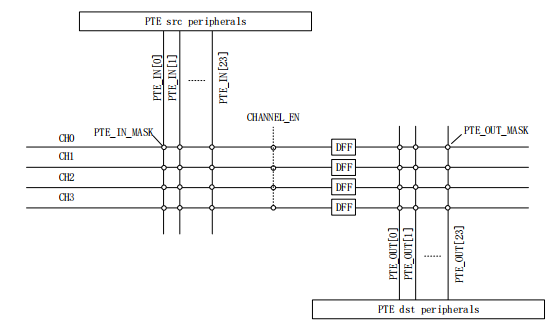
\includegraphics[width=1\linewidth]{./img/PTE/PTE_structure} 

}

\caption{PTE原理图}\label{fig:PTE}
\end{figure}

\hypertarget{ux529fux80fd}{%
\subsection{功能}\label{ux529fux80fd}}

PTE具有不同外设之间的可编程内部通道,可以从src外设触发dst外设。PTE可以不依赖CPU而通过硬件的方式触发任务,因此任务可以在同步DFF所占用的周期内启动。

src外设通过pte\_in\_mask配置,dst外设通过pte\_out\_mask配置。在SOC中集成了4个PTE通道,每个通道可以通过通道使能信号来启用/禁用。

当DFF为高时PTE中断将挂起。在清除PTE中断之前,src外设中断必须被清除,否则另一个启动脉冲将发送到dst外设,这可能会产生未知的错误。

\hypertarget{ux4f7fux7528ux65b9ux6cd5-3}{%
\section{使用方法}\label{ux4f7fux7528ux65b9ux6cd5-3}}

\hypertarget{ux65b9ux6cd5ux6982ux8ff0-3}{%
\subsection{方法概述}\label{ux65b9ux6cd5ux6982ux8ff0-3}}

PTE使用方法总结为:建议不使用PTE中断,在dst外设中断里清PTE中断(或关闭PTE通道)。

\textbf{1.} 配置触发外设和被触发外设以及相应中断(被触发外设中断一定要有)

\textbf{2.} 配置要使用的PTE通道寄存器以及中断(建议不使用PTE中断)

\textbf{3.} 使能触发外设,等待PTE中断(如定义)和被触发外设来中断

\textbf{4.} 在PTE中断中清PTE mask(如定义)

\textbf{5.} 在被触发外设中断中清PTE中断(如定义),如果只触发一次则直接关闭PTE通道

\hypertarget{ux6ce8ux610fux70b9-3}{%
\subsection{注意点}\label{ux6ce8ux610fux70b9-3}}

\begin{itemize}
\item
  不清src中断会循环通过PTE触发dst外设,使程序陷入死循环
\item
  不清PTE中断会循环触发dst外设,使程序陷入死循环
\item
  PTE中断优先级低容易被打断,在极端情况下如果dst外设来中断非常快会出问题(一般不会)
\item
  使用PTE中断会更多占用CPU资源并增加触发过程操作复杂度、增加出错风险,中断处理程序完全可以在src和dst中断中完成,所以强烈建议不要使用PTE中断
\end{itemize}

\hypertarget{ux7f16ux7a0bux6307ux5357-3}{%
\section{编程指南}\label{ux7f16ux7a0bux6307ux5357-3}}

\hypertarget{srcdstux5916ux8bbe}{%
\subsection{src\&dst外设}\label{srcdstux5916ux8bbe}}

当前PTE支持的src外设定义在SYSCTRL\_PTE\_SRC\_INT中:

\begin{Shaded}
\begin{Highlighting}[]
\KeywordTok{typedef} \KeywordTok{enum}
\NormalTok{\{}
\NormalTok{    SYSCTRL_PTE_I2C0_INT       = }\DecValTok{0}\NormalTok{,}
\NormalTok{    SYSCTRL_PTE_I2C1_INT       = }\DecValTok{1}\NormalTok{,}
\NormalTok{    SYSCTRL_PTE_SARADC_INT     = }\DecValTok{2}\NormalTok{,}
\NormalTok{    SYSCTRL_PTE_I2S_INT        = }\DecValTok{3}\NormalTok{,}
\NormalTok{    SYSCTRL_PTE_DMA_INT        = }\DecValTok{4}\NormalTok{,}
\NormalTok{    SYSCTRL_PTE_IR_INT         = }\DecValTok{5}\NormalTok{,}
\NormalTok{    SYSCTRL_PTE_KEYSCANNER_INT = }\DecValTok{6}\NormalTok{,}
\NormalTok{    SYSCTRL_PTE_PWMC0_INT      = }\DecValTok{7}\NormalTok{,}
\NormalTok{    SYSCTRL_PTE_PWMC1_INT      = }\DecValTok{8}\NormalTok{,}
\NormalTok{    SYSCTRL_PTE_PWMC2_INT      = }\DecValTok{9}\NormalTok{,}
\NormalTok{    SYSCTRL_PTE_TIMER0_INT     = }\DecValTok{10}\NormalTok{,}
\NormalTok{    SYSCTRL_PTE_TIMER1_INT     = }\DecValTok{11}\NormalTok{,}
\NormalTok{    SYSCTRL_PTE_TIMER2_INT     = }\DecValTok{12}\NormalTok{,}
\NormalTok{    SYSCTRL_PTE_GPIO0_INT      = }\DecValTok{13}\NormalTok{,}
\NormalTok{    SYSCTRL_PTE_GPIO1_INT      = }\DecValTok{14}\NormalTok{,}
\NormalTok{    SYSCTRL_PTE_UART0_INT      = }\DecValTok{15}\NormalTok{,}
\NormalTok{    SYSCTRL_PTE_UART1_INT      = }\DecValTok{16}\NormalTok{,}
\NormalTok{    SYSCTRL_PTE_SPI0_INT       = }\DecValTok{17}\NormalTok{,}
\NormalTok{    SYSCTRL_PTE_SPI1_INT       = }\DecValTok{18}\NormalTok{,}
\NormalTok{    SYSCTRL_PTE_SPIFLASH       = }\DecValTok{19}\NormalTok{,}
\NormalTok{    SYSCTRL_PTE_RCT_CNT        = }\DecValTok{20}\NormalTok{,}
\NormalTok{    SYSCTRL_PTE_IR_WAKEUP      = }\DecValTok{21}\NormalTok{,}
\NormalTok{    SYSCTRL_PTE_USB_INT        = }\DecValTok{22}\NormalTok{,}
\NormalTok{    SYSCTRL_PTE_QDEC_INT       = }\DecValTok{23}\NormalTok{,}

\NormalTok{    SYSCTRL_PTE_SRC_INT_MAX    = }\DecValTok{24}\NormalTok{,}
\NormalTok{\} SYSCTRL_PTE_SRC_INT;}
\end{Highlighting}
\end{Shaded}

dst外设定义在SYSCTRL\_PTE\_DST\_EN中:

\begin{Shaded}
\begin{Highlighting}[]
\KeywordTok{typedef} \KeywordTok{enum}
\NormalTok{\{}
\NormalTok{    SYSCTRL_PTE_I2C0_EN        = }\DecValTok{0}\NormalTok{,}
\NormalTok{    SYSCTRL_PTE_I2C1_EN        = }\DecValTok{1}\NormalTok{,}
\NormalTok{    SYSCTRL_PTE_SARADC_EN      = }\DecValTok{2}\NormalTok{,}
\NormalTok{    SYSCTRL_PTE_I2S_TX_EN      = }\DecValTok{3}\NormalTok{,}
\NormalTok{    SYSCTRL_PTE_I2S_RX_EN      = }\DecValTok{4}\NormalTok{,}
\NormalTok{    SYSCTRL_PTE_IR_EN          = }\DecValTok{5}\NormalTok{,}
\NormalTok{    SYSCTRL_PTE_KEYSCANNER_EN  = }\DecValTok{6}\NormalTok{,}
\NormalTok{    SYSCTRL_PTE_PWMC0_EN       = }\DecValTok{7}\NormalTok{,}
\NormalTok{    SYSCTRL_PTE_PWMC1_EN       = }\DecValTok{8}\NormalTok{,}
\NormalTok{    SYSCTRL_PTE_PWMC2_EN       = }\DecValTok{9}\NormalTok{,}
\NormalTok{    SYSCTRL_PTE_TIMER0_CH0_EN  = }\DecValTok{10}\NormalTok{,}
\NormalTok{    SYSCTRL_PTE_TIMER0_CH1_EN  = }\DecValTok{11}\NormalTok{,}
\NormalTok{    SYSCTRL_PTE_TIMER1_CH0_EN  = }\DecValTok{12}\NormalTok{,}
\NormalTok{    SYSCTRL_PTE_TIMER1_CH1_EN  = }\DecValTok{13}\NormalTok{,}
\NormalTok{    SYSCTRL_PTE_TIMER2_CH0_EN  = }\DecValTok{14}\NormalTok{,}
\NormalTok{    SYSCTRL_PTE_TIMER2_CH1_EN  = }\DecValTok{15}\NormalTok{,}

\NormalTok{    SYSCTRL_PTE_DST_EN_MAX     = }\DecValTok{16}\NormalTok{,}
\NormalTok{\} SYSCTRL_PTE_DST_EN;}
\end{Highlighting}
\end{Shaded}

通过PTE连接的src外设和dst外设需要在已注册枚举中选取。

\hypertarget{ux9a71ux52a8ux63a5ux53e3-3}{%
\subsection{驱动接口}\label{ux9a71ux52a8ux63a5ux53e3-3}}

\begin{itemize}
\item
  PTE\_ConnectPeripheral:PTE外设连接接口
\item
  PTE\_EnableChennel:PTE通道使能接口
\item
  PTE\_ChennelClose:PTE通道关闭接口
\item
  PTE\_IrqProcess:PTE标准中断程序接口
\item
  PTE\_OutPeripheralContinueProcess:dst外设中断标准PTE中继触发接口
\item
  PTE\_OutPeripheralEndProcess:dst外设中断标准PTE结束接口
\end{itemize}

\hypertarget{ux4ee3ux7801ux793aux4f8b-3}{%
\subsection{代码示例}\label{ux4ee3ux7801ux793aux4f8b-3}}

下面以Timer0通过PTE通道0触发Timer1为例展示PTE的具体使用方法。

src外设和dst外设配置方法不在本文档介绍范围内,我们默认Timer0和Timer1已经配置好并注册好中断。

\begin{Shaded}
\begin{Highlighting}[]
\DataTypeTok{uint32_t}\NormalTok{ Timer0Isr(}\DataTypeTok{void}\NormalTok{ *user_data)}
\NormalTok{\{}
\NormalTok{    TMR_IntClr(APB_TMR0);}
    \ControlFlowTok{return} \DecValTok{0}\NormalTok{;}
\NormalTok{\}}

\DataTypeTok{uint32_t}\NormalTok{ Timer1Isr(}\DataTypeTok{void}\NormalTok{ *user_data)}
\NormalTok{\{}
\NormalTok{    TMR_IntClr(APB_TMR1);}
\NormalTok{    PTE_OutPeripheralContinueProcess(}\DecValTok{0}\NormalTok{);}
    \ControlFlowTok{return} \DecValTok{0}\NormalTok{;}
\NormalTok{\}}

\CommentTok{// 仅供参考,不建议注册PTE中断}
\DataTypeTok{uint32_t}\NormalTok{ PTE0Isr(}\DataTypeTok{void}\NormalTok{ *user_data)}
\NormalTok{\{}
\NormalTok{    PTE_IrqProcess(}\DecValTok{0}\NormalTok{);}
    \ControlFlowTok{return} \DecValTok{0}\NormalTok{;}
\NormalTok{\}}

\DataTypeTok{void}\NormalTok{ PTE_Test(}\DataTypeTok{void}\NormalTok{)}
\NormalTok{\{}
\NormalTok{    PTE_ConnectPeripheral(SYSCTRL_PTE_CHENNEL_0, }
\NormalTok{                          SYSCTRL_PTE_TIMER0_INT, }
\NormalTok{                          SYSCTRL_PTE_TIMER1_CH0_EN);}
\NormalTok{    TMR_Enable(APB_TMR0);}
\NormalTok{\}}
\end{Highlighting}
\end{Shaded}

上面示例会保留PTE通道0并等待下一次触发。如果想要触发之后直接关闭通道代码如下:

\begin{Shaded}
\begin{Highlighting}[]
\DataTypeTok{uint32_t}\NormalTok{ Timer1Isr(}\DataTypeTok{void}\NormalTok{ *user_data)}
\NormalTok{\{}
\NormalTok{    TMR_IntClr(APB_TMR1);}
\NormalTok{    PTE_OutPeripheralEndProcess(}\DecValTok{0}\NormalTok{);}
    \ControlFlowTok{return} \DecValTok{0}\NormalTok{;}
\NormalTok{\}}
\end{Highlighting}
\end{Shaded}

关闭通道会断开Timer0和Timer1的连接,再次触发需要重新建立连接。

\hypertarget{ch-pwm}{%
\chapter{增强型脉宽调制发生器(PWM)}\label{ch-pwm}}

增强型脉宽调制发生器具有两大功能:生成脉宽调制信号(PWM),捕捉外部脉冲输入(PCAP)。
增强型脉宽调制发生器具备 3 个通道,每个通道都可以单独配置为 PWM 或者 PCAP 模式。
每个通道拥有独立的 FIFO。FIFO 里的每个存储单元为 2 个 20bit 数据。
FIFO 深度为 4,即最多存储 4 个单元,共 \(8 \times 20bit\) 数据。
这里的 20bit 位宽是因为本硬件模块内部 PWM 使用的各计数器都是 20 比特。
可根据 FIFO 内的数据量触发中断或者 DMA 传输。

说明:\protect\hyperlink{ch-timer}{TIMER} 也支持生成脉宽调制信号,但是可配置的参数较简单,不支持死区等。

PWM 特性:

\begin{itemize}
\tightlist
\item
  最多支持 3 个 PWM 通道,每一个通道包含 A、B 两个输出
\item
  每个通道参数独立
\item
  支持死区
\item
  支持通过 DMA 更新 PWM 配置
\end{itemize}

PCAP 特性:

\begin{itemize}
\tightlist
\item
  支持 3 个 PCAP 通道,每一个通道包含两个输入
\item
  支持捕捉上升沿、下降沿
\item
  支持通过 DMA 读取数据
\end{itemize}

\hypertarget{pwm-ux5de5ux4f5cux6a21ux5f0f}{%
\section{PWM 工作模式}\label{pwm-ux5de5ux4f5cux6a21ux5f0f}}

PWM 使用的时钟频率可配置,请参考 \protect\hyperlink{ch-sysctrl}{SYSCTRL}。

每个 PWM 通道支持以下多种工作模式:

\begin{Shaded}
\begin{Highlighting}[]
\KeywordTok{typedef} \KeywordTok{enum}
\NormalTok{\{}
\NormalTok{    ..._UP_WITHOUT_DIED_ZONE          = ...,}
\NormalTok{    ..._UP_WITH_DIED_ZONE             = ...,}
\NormalTok{    ..._UPDOWN_WITHOUT_DIED_ZONE      = ...,}
\NormalTok{    ..._UPDOWN_WITH_DIED_ZONE         = ...,}
\NormalTok{    ..._SINGLE_WITHOUT_DIED_ZONE      = ...,}
\NormalTok{    ..._DMA                           = ...,}
\NormalTok{\} PWM_WorkMode_t;}
\end{Highlighting}
\end{Shaded}

\hypertarget{ux6700ux7b80ux5355ux7684ux6a21ux5f0fup_without_died_zone}{%
\subsection{最简单的模式:UP\_WITHOUT\_DIED\_ZONE}\label{ux6700ux7b80ux5355ux7684ux6a21ux5f0fup_without_died_zone}}

此模式需要配置两个门限:计数器回零门限 PERA\_TH、高门限 HIGH\_TH,HIGH\_TH
必须小于 HIGH\_TH。以伪代码描述 A、B 输出如下:

\begin{Shaded}
\begin{Highlighting}[]
\NormalTok{cnt = }\DecValTok{0}\NormalTok{;}
\NormalTok{on_clock_rising_edge()}
\NormalTok{\{}
\NormalTok{    cnt = cnt < PERA_TH ? cnt + }\DecValTok{1}\NormalTok{ : }\DecValTok{0}\NormalTok{;}
\NormalTok{    A = HIGH_TH <= cnt;}
\NormalTok{    B = !A;}
\NormalTok{\}}
\end{Highlighting}
\end{Shaded}

\hypertarget{up_with_died_zone}{%
\subsection{UP\_WITH\_DIED\_ZONE}\label{up_with_died_zone}}

与 UP\_WITHOUT\_DIED\_ZONE 相比,此模式需要一个新的死区门限 DZONE\_TH,DZONE\_TH
必须小于 HIGH\_TH。以伪代码描述 A、B 输出如下:

cnt = 0;
on\_clock\_rising\_edge()
\{
cnt = cnt \textless{} PERA\_TH ? cnt + 1 : 0;
A = HIGH\_TH + DZONE\_TH \textless= cnt;
B = DZONE\_TH \textless= cnt \textless{} HIGH\_TH);
\}

\hypertarget{updown_without_died_zone}{%
\subsection{UPDOWN\_WITHOUT\_DIED\_ZONE}\label{updown_without_died_zone}}

此模式需要的门限参数与 UP\_WITHOUT\_DIED\_ZONE 相同。以伪代码描述 A、B 输出如下:

\begin{Shaded}
\begin{Highlighting}[]
\NormalTok{cnt = }\DecValTok{0}\NormalTok{;}
\NormalTok{on_clock_rising_edge()}
\NormalTok{\{}
\NormalTok{    cnt = cnt < }\DecValTok{2}\NormalTok{ * PERA_TH ? cnt + }\DecValTok{1}\NormalTok{ : }\DecValTok{0}\NormalTok{;}
\NormalTok{    A = PERA_TH - HIGH_TH <= cnt <= PERA_TH + HIGH_TH;}
\NormalTok{    B = !A;}
\NormalTok{\}}
\end{Highlighting}
\end{Shaded}

\hypertarget{updown_with_died_zone}{%
\subsection{UPDOWN\_WITH\_DIED\_ZONE}\label{updown_with_died_zone}}

与 UP\_WITHOUT\_DIED\_ZONE 相比,此模式需要一个新的死区门限 DZONE\_TH。
以伪代码描述 A、B 输出如下:

\begin{Shaded}
\begin{Highlighting}[]
\NormalTok{cnt = }\DecValTok{0}\NormalTok{;}
\NormalTok{on_clock_rising_edge()}
\NormalTok{\{}
\NormalTok{    cnt = cnt < }\DecValTok{2}\NormalTok{ * PERA_TH ? cnt + }\DecValTok{1}\NormalTok{ : }\DecValTok{0}\NormalTok{;}
\NormalTok{    A = PERA_TH - HIGH_TH + DZONE_TH <= cnt <= PERA_TH + HIGH_TH;}
\NormalTok{    B = (cnt < PERA_TH - HIGH_TH) || (cnt > PERA_TH + HIGH_TH + DZONE_TH);}
\NormalTok{\}}
\end{Highlighting}
\end{Shaded}

\hypertarget{single_without_died_zone}{%
\subsection{SINGLE\_WITHOUT\_DIED\_ZONE}\label{single_without_died_zone}}

此模式需要配置两个门限:计数器回零门限 PERA\_TH、高门限 HIGH\_TH,HIGH\_TH
必须小于 HIGH\_TH。此模式只产生一个脉冲,以伪代码描述 A、B 输出如下:

\begin{Shaded}
\begin{Highlighting}[]
\NormalTok{cnt = }\DecValTok{0}\NormalTok{;}
\NormalTok{on_clock_rising_edge()}
\NormalTok{\{}
\NormalTok{    cnt++;}
\NormalTok{    A = HIGH_TH <= cnt < PERA_TH;}
\NormalTok{    B = !A;}
\NormalTok{\}}
\end{Highlighting}
\end{Shaded}

\begin{rmdcaution}
以上伪代码仅用于辅助描述硬件行为,与实际行为可以存在微小差异。
\end{rmdcaution}

\hypertarget{dma-ux6a21ux5f0f}{%
\subsection{DMA 模式}\label{dma-ux6a21ux5f0f}}

此模式支持通过 DMA 实时更新门限。

\hypertarget{ux8f93ux51faux63a7ux5236}{%
\subsection{输出控制}\label{ux8f93ux51faux63a7ux5236}}

对于每个通道的每一路输出,另有 3 个参数控制最终的两路输出:掩膜、停机输出值、反相。
最终的输出以伪代码描述如下:

\begin{Shaded}
\begin{Highlighting}[]
\NormalTok{output_control(v)}
\NormalTok{\{}
    \ControlFlowTok{if}\NormalTok{ (掩膜 == }\DecValTok{1}\NormalTok{) }\ControlFlowTok{return}\NormalTok{ A 路输出 }\DecValTok{0}\NormalTok{、B 路输出 }\DecValTok{1}\NormalTok{;}
    \ControlFlowTok{if}\NormalTok{ (本通道已停机) }\ControlFlowTok{return}\NormalTok{ 停机输出值;}
    \ControlFlowTok{if}\NormalTok{ (反相) v = !v;}
    \ControlFlowTok{return}\NormalTok{ v;}
\NormalTok{\}}
\end{Highlighting}
\end{Shaded}

\hypertarget{pcap}{%
\section{PCAP}\label{pcap}}

PCAP 每个通道包含两路输入。PCAP 内部有一个单独的 32 比特计数器\footnote{所有 6 路输入共有此计数器。},
当检测到输入信号变化(包含上升沿和下降沿)时,PCAP 将计数器的值及边沿变化信息作为一个存储单元压入
FIFO:

\begin{Shaded}
\begin{Highlighting}[]
\KeywordTok{struct}\NormalTok{ data0}
\NormalTok{\{}
    \DataTypeTok{uint32_t}\NormalTok{ cnt_high:}\DecValTok{12}\NormalTok{;}
    \DataTypeTok{uint32_t}\NormalTok{ p_cap_0_p:}\DecValTok{1}\NormalTok{; }\CommentTok{// A 路出现上升沿}
    \DataTypeTok{uint32_t}\NormalTok{ p_cap_0_n:}\DecValTok{1}\NormalTok{; }\CommentTok{// A 路出现下降沿}
    \DataTypeTok{uint32_t}\NormalTok{ p_cap_1_p:}\DecValTok{1}\NormalTok{; }\CommentTok{// B 路出现上升沿}
    \DataTypeTok{uint32_t}\NormalTok{ p_cap_1_n:}\DecValTok{1}\NormalTok{; }\CommentTok{// B 路出现下降沿}
    \DataTypeTok{uint32_t}\NormalTok{ tag:}\DecValTok{4}\NormalTok{;}
    \DataTypeTok{uint32_t}\NormalTok{ padding:}\DecValTok{12}\NormalTok{;}
\NormalTok{\};}
\KeywordTok{struct}\NormalTok{ data1}
\NormalTok{\{}
    \DataTypeTok{uint32_t}\NormalTok{ cnt_low:}\DecValTok{20}\NormalTok{;}
    \DataTypeTok{uint32_t}\NormalTok{ padding:}\DecValTok{12}\NormalTok{;}
\NormalTok{\};}
\end{Highlighting}
\end{Shaded}

通过复位整个模块可以清零 PCAP 计数器。

\hypertarget{pwm-ux4f7fux7528ux8bf4ux660e}{%
\section{PWM 使用说明}\label{pwm-ux4f7fux7528ux8bf4ux660e}}

\hypertarget{ux542fux52a8ux4e0eux505cux6b62}{%
\subsection{启动与停止}\label{ux542fux52a8ux4e0eux505cux6b62}}

共有两个开关与 PWM 的启动和停止有关:使能(Enable)、停机控制(HaltCtrl)。只有当 \texttt{Enable} 为 1,
\texttt{HaltCtrl} 为 0 时,PWM 才真正开始工作。

相关的 API 为:

\begin{Shaded}
\begin{Highlighting}[]
\CommentTok{// 使能 PWM 通道}
\DataTypeTok{void}\NormalTok{ PWM_Enable(}
    \DataTypeTok{const} \DataTypeTok{uint8_t}\NormalTok{ channel_index,    }\CommentTok{// 通道号}
    \DataTypeTok{const} \DataTypeTok{uint8_t}\NormalTok{ enable            }\CommentTok{// 使能或禁用}
\NormalTok{    );}

\CommentTok{// PWM 通道停机控制}
\DataTypeTok{void}\NormalTok{ PWM_HaltCtrlEnable(}
    \DataTypeTok{const} \DataTypeTok{uint8_t}\NormalTok{ channel_index,    }\CommentTok{// 通道号}
    \DataTypeTok{const} \DataTypeTok{uint8_t}\NormalTok{ enable            }\CommentTok{// 停机(1) 或运转(0)}
\NormalTok{    );}
\end{Highlighting}
\end{Shaded}

\hypertarget{ux914dux7f6eux5de5ux4f5cux6a21ux5f0f}{%
\subsection{配置工作模式}\label{ux914dux7f6eux5de5ux4f5cux6a21ux5f0f}}

\begin{Shaded}
\begin{Highlighting}[]
\DataTypeTok{void}\NormalTok{ PWM_SetMode(}
    \DataTypeTok{const} \DataTypeTok{uint8_t}\NormalTok{ channel_index,    }\CommentTok{// 通道号}
    \DataTypeTok{const}\NormalTok{ PWM_WorkMode_t mode       }\CommentTok{// 模式}
\NormalTok{    );}
\end{Highlighting}
\end{Shaded}

\hypertarget{ux914dux7f6eux95e8ux9650}{%
\subsection{配置门限}\label{ux914dux7f6eux95e8ux9650}}

\begin{Shaded}
\begin{Highlighting}[]
\CommentTok{// 配置 PERA_TH}
\DataTypeTok{void}\NormalTok{ PWM_SetPeraThreshold(}
    \DataTypeTok{const} \DataTypeTok{uint8_t}\NormalTok{ channel_index,}
    \DataTypeTok{const} \DataTypeTok{uint32_t}\NormalTok{ threshold);}
\end{Highlighting}
\end{Shaded}

\begin{Shaded}
\begin{Highlighting}[]
\CommentTok{// 配置 DZONE_TH}
\DataTypeTok{void}\NormalTok{ PWM_SetDiedZoneThreshold(}
    \DataTypeTok{const} \DataTypeTok{uint8_t}\NormalTok{ channel_index,}
    \DataTypeTok{const} \DataTypeTok{uint32_t}\NormalTok{ threshold);}
\end{Highlighting}
\end{Shaded}

\begin{Shaded}
\begin{Highlighting}[]
\CommentTok{// 配置 HIGH_TH}
\DataTypeTok{void}\NormalTok{ PWM_SetHighThreshold(}
    \DataTypeTok{const} \DataTypeTok{uint8_t}\NormalTok{ channel_index,}
    \DataTypeTok{const} \DataTypeTok{uint8_t}\NormalTok{ multi_duty_index, }\CommentTok{// 对于 ING916XX,此参数无效}
    \DataTypeTok{const} \DataTypeTok{uint32_t}\NormalTok{ threshold);}
\end{Highlighting}
\end{Shaded}

各门限值最大支持 0xFFFFF,共 20 个比特。

\hypertarget{ux8f93ux51faux63a7ux5236-1}{%
\subsection{输出控制}\label{ux8f93ux51faux63a7ux5236-1}}

\begin{Shaded}
\begin{Highlighting}[]
\CommentTok{// 掩膜控制}
\DataTypeTok{void}\NormalTok{ PWM_SetMask(}
    \DataTypeTok{const} \DataTypeTok{uint8_t}\NormalTok{ channel_index,    }\CommentTok{// 通道号}
    \DataTypeTok{const} \DataTypeTok{uint8_t}\NormalTok{ mask_a,           }\CommentTok{// A 路掩膜}
    \DataTypeTok{const} \DataTypeTok{uint8_t}\NormalTok{ mask_b            }\CommentTok{// B 路掩膜}
\NormalTok{    );}
\end{Highlighting}
\end{Shaded}

\begin{Shaded}
\begin{Highlighting}[]
\CommentTok{// 配置停机输出值}
\DataTypeTok{void}\NormalTok{ PWM_HaltCtrlCfg(}
    \DataTypeTok{const} \DataTypeTok{uint8_t}\NormalTok{ channel_index,    }\CommentTok{// 通道号}
    \DataTypeTok{const} \DataTypeTok{uint8_t}\NormalTok{ out_a,            }\CommentTok{// A 路停机输出值}
    \DataTypeTok{const} \DataTypeTok{uint8_t}\NormalTok{ out_b             }\CommentTok{// B 路停机输出值}
\NormalTok{    );}
\end{Highlighting}
\end{Shaded}

\begin{Shaded}
\begin{Highlighting}[]
\CommentTok{// 反相}
\DataTypeTok{void}\NormalTok{ PWM_SetInvertOutput(}
    \DataTypeTok{const} \DataTypeTok{uint8_t}\NormalTok{ channel_index,    }\CommentTok{// 通道号}
    \DataTypeTok{const} \DataTypeTok{uint8_t}\NormalTok{ inv_a,            }\CommentTok{// A 路是否反相}
    \DataTypeTok{const} \DataTypeTok{uint8_t}\NormalTok{ inv_b             }\CommentTok{// B 路是否反相}
\NormalTok{    );}
\end{Highlighting}
\end{Shaded}

\hypertarget{ux7efcux5408ux793aux4f8b} 的方波,
涉及 3 个关键参数:

\begin{itemize}
\item
  生成这种最简单的 PWM 信号需要的模式为 UP\_WITHOUT\_DIED\_ZONE;
\item
  PERA\_TH 控制输出信号的频率,设置为 \texttt{PWM\_CLOCK\_FREQ\ /\ frequency};
\item
  HIGH\_TH 控制信号的占空比,设置为 \texttt{PERA\_TH\ *\ (100\ -\ on\_duty)\ \%}
\end{itemize}

\begin{Shaded}
\begin{Highlighting}[]
\DataTypeTok{void}\NormalTok{ PWM_SetupSimple(}
    \DataTypeTok{const} \DataTypeTok{uint8_t}\NormalTok{ channel_index,}
    \DataTypeTok{const} \DataTypeTok{uint32_t}\NormalTok{ frequency,}
    \DataTypeTok{const} \DataTypeTok{uint16_t}\NormalTok{ on_duty)}
\NormalTok{\{}
    \DataTypeTok{uint32_t}\NormalTok{ pera = PWM_CLOCK_FREQ / frequency;}
    \DataTypeTok{uint32_t}\NormalTok{ high = pera > }\DecValTok{1000}\NormalTok{ ?}
\NormalTok{          pera / }\DecValTok{100}\NormalTok{ * (}\DecValTok{100}\NormalTok{ - on_duty)}
\NormalTok{        : pera * (}\DecValTok{100}\NormalTok{ - on_duty) / }\DecValTok{100}\NormalTok{;}
\NormalTok{    PWM_HaltCtrlEnable(channel_index, }\DecValTok{1}\NormalTok{);}
\NormalTok{    PWM_Enable(channel_index, }\DecValTok{0}\NormalTok{);}
\NormalTok{    PWM_SetPeraThreshold(channel_index, pera);}
\NormalTok{    PWM_SetHighThreshold(channel_index, }\DecValTok{0}\NormalTok{, high);}
\NormalTok{    PWM_SetMode(channel_index, PWM_WORK_MODE_UP_WITHOUT_DIED_ZONE);}
\NormalTok{    PWM_SetMask(channel_index, }\DecValTok{0}\NormalTok{, }\DecValTok{0}\NormalTok{);}
\NormalTok{    PWM_Enable(channel_index, }\DecValTok{1}\NormalTok{);}
\NormalTok{    PWM_HaltCtrlEnable(channel_index, }\DecValTok{0}\NormalTok{);}
\NormalTok{\}}
\end{Highlighting}
\end{Shaded}

\hypertarget{ux4f7fux7528-dma-ux5b9eux65f6ux66f4ux65b0ux914dux7f6e}{%
\subsection{使用 DMA 实时更新配置}\label{ux4f7fux7528-dma-ux5b9eux65f6ux66f4ux65b0ux914dux7f6e}}

使用 DMA 能够实时更新配置(相当于工作在 UP\_WITHOUT\_DIED\_ZONE,但是每个循环使用不同的参数):
每当 PWM 计数器计完一圈回零时,自动使用来自 DMA 的数据更新配置。
这些数据以 2 个 \texttt{uint32\_t} 为一组,依次表示 HIGH\_TH 和 PERA\_TH。

\begin{Shaded}
\begin{Highlighting}[]
\DataTypeTok{void}\NormalTok{ PWM_DmaEnable(}
    \DataTypeTok{const} \DataTypeTok{uint8_t}\NormalTok{ channel_index, }\CommentTok{// 通道号}
    \DataTypeTok{uint8_t}\NormalTok{ trig_cfg,            }\CommentTok{// DMA 请求触发门限}
    \DataTypeTok{uint8_t}\NormalTok{ enable               }\CommentTok{// 使能}
\NormalTok{    );}
\end{Highlighting}
\end{Shaded}

当 PWM 内部 FIFO 数据少于 \texttt{trig\_cfg},PWM 请求 DMA 传输数据。PWM FIFO 深度为 4(指可以存储 4 组 PWM 配置),
所以 \texttt{trig\_cfg} 的取值范围为 \(1..4\)。

\hypertarget{pcap-ux4f7fux7528ux8bf4ux660e}{%
\section{PCAP 使用说明}\label{pcap-ux4f7fux7528ux8bf4ux660e}}

\hypertarget{ux914dux7f6e-pcap-ux6a21ux5f0f}{%
\subsection{配置 PCAP 模式}\label{ux914dux7f6e-pcap-ux6a21ux5f0f}}

要启用 PCAP 模式,需要 5 个步骤:

\begin{enumerate}
\def\labelenumi{\arabic{enumi}.}
\item
  关闭整个模块的时钟(参考 \protect\hyperlink{ch-sysctrl}{SYSCTRL})
\item
  使用 \texttt{PCAP\_Enable} 使能 PCAP 模式

\begin{Shaded}
\begin{Highlighting}[]
\DataTypeTok{void}\NormalTok{ PCAP_Enable(}
    \DataTypeTok{const} \DataTypeTok{uint8_t}\NormalTok{ channel_index     }\CommentTok{// 通道号}
\NormalTok{);}
\end{Highlighting}
\end{Shaded}
\item
  使用 \texttt{PCAP\_EnableEvents} 选择要检测的事件

\begin{Shaded}
\begin{Highlighting}[]
\DataTypeTok{void}\NormalTok{ PCAP_EnableEvents(}
    \DataTypeTok{const} \DataTypeTok{uint8_t}\NormalTok{ channel_index,}
    \DataTypeTok{uint8_t}\NormalTok{ events_on_0,}
    \DataTypeTok{uint8_t}\NormalTok{ events_on_1);}
\end{Highlighting}
\end{Shaded}

  \texttt{events} 为下面两个事件的组合:

\begin{Shaded}
\begin{Highlighting}[]
\KeywordTok{enum}\NormalTok{ PCAP_PULSE_EVENT}
\NormalTok{\{}
\NormalTok{    PCAP_PULSE_RISING_EDGE  = }\BaseNTok{0x1}\NormalTok{,}
\NormalTok{    PCAP_PULSE_FALLING_EDGE = }\BaseNTok{0x2}\NormalTok{,}
\NormalTok{\};}
\end{Highlighting}
\end{Shaded}

  比如在通道 1 的 A 路输入上同时检测、上报上升沿和下降沿:

\begin{Shaded}
\begin{Highlighting}[]
\NormalTok{PCAP_EnableEvents(}\DecValTok{1}\NormalTok{,}
\NormalTok{    PCAP_PULSE_RISING_EDGE}
\NormalTok{    | PCAP_PULSE_FALLING_EDGE,}
\NormalTok{    ...);}
\end{Highlighting}
\end{Shaded}
\item
  打开整个模块的时钟(参考 \protect\hyperlink{ch-sysctrl}{SYSCTRL})
\item
  配置 DMA 传输

  当 PCAP 通道 FIFO 内存储的数据多于 \texttt{trig\_cfg},请求 DMA 传输数据。\texttt{trig\_cfg} 的取值范围为 \(0..4\)。

\begin{Shaded}
\begin{Highlighting}[]
\DataTypeTok{void}\NormalTok{ PCAP_DmaEnable(}
    \DataTypeTok{const} \DataTypeTok{uint8_t}\NormalTok{ channel_index, }\CommentTok{// 通道号}
    \DataTypeTok{uint8_t}\NormalTok{ trig_cfg,            }\CommentTok{// DMA 请求触发门限}
    \DataTypeTok{uint8_t}\NormalTok{ enable               }\CommentTok{// 使能}
\NormalTok{    );}
\end{Highlighting}
\end{Shaded}
\item
  使能计数器

\begin{Shaded}
\begin{Highlighting}[]
\DataTypeTok{void}\NormalTok{ PCAP_CounterEnable(}
    \DataTypeTok{uint8_t}\NormalTok{ enable              }\CommentTok{// 使能(1)/禁用(0)}
\NormalTok{    );}
\end{Highlighting}
\end{Shaded}
\end{enumerate}

\hypertarget{ux8bfbux53d6ux8ba1ux6570ux5668}{%
\subsection{读取计数器}\label{ux8bfbux53d6ux8ba1ux6570ux5668}}

\begin{Shaded}
\begin{Highlighting}[]
\DataTypeTok{uint32_t}\NormalTok{ PCAP_ReadCounter(}\DataTypeTok{void}\NormalTok{);}
\end{Highlighting}
\end{Shaded}

\hypertarget{ch-rtc}{%
\chapter{实时时钟(RTC)}\label{ch-rtc}}

\hypertarget{ux529fux80fdux63cfux8ff0-4}{%
\section{功能描述}\label{ux529fux80fdux63cfux8ff0-4}}

实时时钟是一个独立的定时器。RTC模块拥有一组连续计数的计数器,在相应的软件配置下,
可提供时钟日历的功能。修改计数器的值可以重新设置系统当前的时间和日期。

\hypertarget{ux4f7fux7528ux8bf4ux660e-4}{%
\section{使用说明}\label{ux4f7fux7528ux8bf4ux660e-4}}

\hypertarget{rtcux4f7fux80fd}{%
\subsection{RTC使能}\label{rtcux4f7fux80fd}}

使用 \texttt{RTC\_Enable} 使能RTC。

\begin{Shaded}
\begin{Highlighting}[]
\DataTypeTok{void}\NormalTok{ RTC_Enable(}\DataTypeTok{uint8_t}\NormalTok{ enable);}
\end{Highlighting}
\end{Shaded}

\hypertarget{ux83b7ux53d6ux5f53ux524dux65e5ux671f}{%
\subsection{获取当前日期}\label{ux83b7ux53d6ux5f53ux524dux65e5ux671f}}

使用 \texttt{RTC\_GetTime} 获取当前时间(包括时分秒)。

\begin{Shaded}
\begin{Highlighting}[]
\DataTypeTok{uint16_t}\NormalTok{ RTC_GetTime(}
  \DataTypeTok{uint8_t}\NormalTok{ *hour, }
  \DataTypeTok{uint8_t}\NormalTok{ *minute, }
  \DataTypeTok{uint8_t}\NormalTok{ *second}
\NormalTok{  );}
\end{Highlighting}
\end{Shaded}

\hypertarget{ux4feeux6539ux65e5ux671f}{%
\subsection{修改日期}\label{ux4feeux6539ux65e5ux671f}}

使用 \texttt{RTC\_ModifyTime} 修改当前时间。

\begin{Shaded}
\begin{Highlighting}[]
\DataTypeTok{void}\NormalTok{ RTC_ModifyTime(}
  \DataTypeTok{uint16_t}\NormalTok{ day, }
  \DataTypeTok{uint8_t}\NormalTok{ hour, }
  \DataTypeTok{uint8_t}\NormalTok{ minute, }
  \DataTypeTok{uint8_t}\NormalTok{ second}
\NormalTok{  );}
\end{Highlighting}
\end{Shaded}

\hypertarget{ux914dux7f6eux95f9ux949f}{%
\subsection{配置闹钟}\label{ux914dux7f6eux95f9ux949f}}

使用 \texttt{RTC\_ConfigAlarm}

\begin{Shaded}
\begin{Highlighting}[]
\DataTypeTok{void}\NormalTok{ RTC_ConfigAlarm(}
  \DataTypeTok{uint8_t}\NormalTok{ hour, }
  \DataTypeTok{uint8_t}\NormalTok{ minute, }
  \DataTypeTok{uint8_t}\NormalTok{ second}
\NormalTok{  );}
\end{Highlighting}
\end{Shaded}

\hypertarget{ux914dux7f6eux4e2dux65adux8bf7ux6c42-1}{%
\subsection{配置中断请求}\label{ux914dux7f6eux4e2dux65adux8bf7ux6c42-1}}

使用 \texttt{RTC\_EnableIRQ} 配置并使能RTC中断请求。

\begin{Shaded}
\begin{Highlighting}[]
\DataTypeTok{void}\NormalTok{ RTC_EnableIRQ(}\DataTypeTok{uint32_t}\NormalTok{ mask);}
\end{Highlighting}
\end{Shaded}

其中的 \texttt{mask} 为RTC中断类型,一共有六种:

\begin{Shaded}
\begin{Highlighting}[]
\KeywordTok{typedef} \KeywordTok{enum}
\NormalTok{\{}
\NormalTok{    RTC_IRQ_ALARM = }\BaseNTok{0x04}\NormalTok{,}
\NormalTok{    RTC_IRQ_DAY = }\BaseNTok{0x08}\NormalTok{,}
\NormalTok{    RTC_IRQ_HOUR = }\BaseNTok{0x10}\NormalTok{,}
\NormalTok{    RTC_IRQ_MINUTE = }\BaseNTok{0x20}\NormalTok{,}
\NormalTok{    RTC_IRQ_SECOND = }\BaseNTok{0x40}\NormalTok{,}
\NormalTok{    RTC_IRQ_HALF_SECOND = }\BaseNTok{0x80}\NormalTok{,}
\NormalTok{\} rtc_irq_t;}
\end{Highlighting}
\end{Shaded}

\begin{itemize}
\item
  例如将 RTC 设置为alarm中断

\begin{Shaded}
\begin{Highlighting}[]
\NormalTok{RTC_EnableIRQ(RTC_IRQ_ALARM);}
\end{Highlighting}
\end{Shaded}
\item
  例如将 RTC 设置为day中断

\begin{Shaded}
\begin{Highlighting}[]
\NormalTok{RTC_EnableIRQ(RTC_IRQ_DAY);}
\end{Highlighting}
\end{Shaded}
\item
  例如将 RTC 设置为hour中断

\begin{Shaded}
\begin{Highlighting}[]
\NormalTok{RTC_EnableIRQ(RTC_IRQ_HOUR);}
\end{Highlighting}
\end{Shaded}
\item
  例如将 RTC 设置为minute中断

\begin{Shaded}
\begin{Highlighting}[]
\NormalTok{RTC_EnableIRQ(RTC_IRQ_MINUTE);}
\end{Highlighting}
\end{Shaded}
\item
  例如将 RTC 设置为second中断

\begin{Shaded}
\begin{Highlighting}[]
\NormalTok{RTC_EnableIRQ(RTC_IRQ_SECOND);}
\end{Highlighting}
\end{Shaded}
\item
  例如将 RTC 设置为half-second中断

\begin{Shaded}
\begin{Highlighting}[]
\NormalTok{RTC_EnableIRQ(RTC_IRQ_HALF_SECOND);}
\end{Highlighting}
\end{Shaded}
\end{itemize}

\hypertarget{ux83b7ux53d6ux5f53ux524dux4e2dux65adux72b6ux6001}{%
\subsection{获取当前中断状态}\label{ux83b7ux53d6ux5f53ux524dux4e2dux65adux72b6ux6001}}

使用 \texttt{RTC\_GetIntState} 获取当前RTC的中断状态。

\begin{Shaded}
\begin{Highlighting}[]
\DataTypeTok{uint32_t}\NormalTok{ RTC_GetIntState(}\DataTypeTok{void}\NormalTok{);}
\end{Highlighting}
\end{Shaded}

\hypertarget{ux6e05ux9664ux4e2dux65ad}{%
\subsection{清除中断}\label{ux6e05ux9664ux4e2dux65ad}}

使用 \texttt{RTC\_ClearIntState} 清除当前RTC的中断状态。

\begin{Shaded}
\begin{Highlighting}[]
\DataTypeTok{void}\NormalTok{ RTC_ClearIntState(}\DataTypeTok{uint32_t}\NormalTok{ state);}
\end{Highlighting}
\end{Shaded}

\hypertarget{ux5904ux7406ux4e2dux65adux72b6ux6001-1}{%
\subsection{处理中断状态}\label{ux5904ux7406ux4e2dux65adux72b6ux6001-1}}

用 \texttt{RTC\_GetIntState} 获取RTC上的中断触发,返回非 0 值表示RTC上产生了中断请求;RTC产生中断后,
需要消除中断状态方可再次触发。利用 \texttt{RTC\_ClearIntState}可清除RTC的中断触发状态。

\hypertarget{spiux529fux80fdux6982ux8ff0}{%
\chapter{SPI功能概述}\label{spiux529fux80fdux6982ux8ff0}}

\begin{itemize}
\tightlist
\item
  两个SPI模块
\item
  支持SPI主\&从模式
\item
  支持Quad SPI,可以执行代码
\item
  独立的RX\&TX FIFO,深度为8个word
\item
  支持DMA
\end{itemize}

\hypertarget{spiux4f7fux7528ux8bf4ux660e}{%
\section{SPI使用说明}\label{spiux4f7fux7528ux8bf4ux660e}}

以下场景中均以SPI1为例,如果需要SPI0则可以根据情况修改

\hypertarget{ux573aux666f1ux53eaux8bfbux53eaux5199ux4e0dux5e26dma}{%
\section{场景1:只读只写不带DMA}\label{ux573aux666f1ux53eaux8bfbux53eaux5199ux4e0dux5e26dma}}

其中SPI主配置为只写模式,SPI从配置为只读模式,CPU操作读写,没有使用DMA 配置之前需要决定使用的GPIO,如果是普通模式,则不需要SPI\_MIC\_WP和SPI\_MIC\_HOLD

\begin{Shaded}
\begin{Highlighting}[]
\PreprocessorTok{#define SPI_MIC_CLK         GIO_GPIO_10}
\PreprocessorTok{#define SPI_MIC_MOSI        GIO_GPIO_11}
\PreprocessorTok{#define SPI_MIC_MISO        GIO_GPIO_12}
\PreprocessorTok{#define SPI_MIC_CS          GIO_GPIO_13}
\PreprocessorTok{#define SPI_MIC_WP          GIO_GPIO_14}
\PreprocessorTok{#define SPI_MIC_HOLD        GIO_GPIO_15}
\end{Highlighting}
\end{Shaded}

\hypertarget{spiux4e3bux914dux7f6e}{%
\subsection{SPI主配置}\label{spiux4e3bux914dux7f6e}}

\hypertarget{ux63a5ux53e3ux914dux7f6e}{%
\subsubsection{接口配置}\label{ux63a5ux53e3ux914dux7f6e}}

\begin{Shaded}
\begin{Highlighting}[]
\DataTypeTok{static} \DataTypeTok{void}\NormalTok{ setup_peripherals_spi_pin(}\DataTypeTok{void}\NormalTok{)}
\NormalTok{\{}
    \CommentTok{// 打开SPI模块时钟}
    \CommentTok{// 此处是以SPI1为例,如果是SPI0则需要更改}
    \CommentTok{// 根据使用的GPIO,选择打开GPIO0或者GPIO1的时钟}
\NormalTok{    SYSCTRL_ClearClkGateMulti(    (}\DecValTok{1}\NormalTok{ << SYSCTRL_ITEM_APB_SPI1)}
\NormalTok{                                | (}\DecValTok{1}\NormalTok{ << SYSCTRL_ITEM_APB_SysCtrl)}
\NormalTok{                                | (}\DecValTok{1}\NormalTok{ << SYSCTRL_ITEM_APB_PinCtrl)}
\NormalTok{                                | (}\DecValTok{1}\NormalTok{ << SYSCTRL_ITEM_APB_GPIO1)}
\NormalTok{                                | (}\DecValTok{1}\NormalTok{ << SYSCTRL_ITEM_APB_GPIO0));}

    \CommentTok{// 设置IO MUX,将GPIO映射成SPI功能,不需要的pin可以使用IO_NOT_A_PIN替代}
\NormalTok{    PINCTRL_SelSpiIn(SPI_PORT_1, SPI_MIC_CLK, SPI_MIC_CS, SPI_MIC_HOLD, SPI_MIC_WP, SPI_MIC_MISO, SPI_MIC_MOSI);}
\NormalTok{    PINCTRL_SetPadMux(SPI_MIC_CLK, IO_SOURCE_SPI1_CLK_OUT);}
\NormalTok{    PINCTRL_SetPadMux(SPI_MIC_CS, IO_SOURCE_SPI1_CSN_OUT);}
\NormalTok{    PINCTRL_SetPadMux(SPI_MIC_MOSI, IO_SOURCE_SPI1_MOSI_OUT);}
    
    \CommentTok{// 设置SPI的中断}
\NormalTok{    platform_set_irq_callback(PLATFORM_CB_IRQ_APBSPI, peripherals_spi_isr, NULL);}
\end{Highlighting}
\end{Shaded}

\hypertarget{spiux6a21ux5757ux521dux59cbux5316}{%
\subsubsection{SPI模块初始化}\label{spiux6a21ux5757ux521dux59cbux5316}}

常用设置项用注释标出,详细定义请参考``peripheral\_ssp.h''

\begin{Shaded}
\begin{Highlighting}[]
\CommentTok{// 示例,每次传输大小是8个word}
\PreprocessorTok{#define DATA_LEN (SPI_FIFO_DEPTH)}
\DataTypeTok{static} \DataTypeTok{void}\NormalTok{ setup_peripherals_spi_module(}\DataTypeTok{void}\NormalTok{)}
\NormalTok{\{}
\NormalTok{    apSSP_sDeviceControlBlock pParam;}
\NormalTok{    pParam.eSclkDiv = SPI_INTERFACETIMINGSCLKDIV_DEFAULT_2M;}\CommentTok{// SPI 时钟设置}
\NormalTok{    pParam.eSCLKPolarity = SPI_CPOL_SCLK_LOW_IN_IDLE_STATES;}\CommentTok{// SPI 模式设置}
\NormalTok{    pParam.eSCLKPhase = SPI_CPHA_ODD_SCLK_EDGES;}\CommentTok{// SPI 模式设置}
\NormalTok{    pParam.eLsbMsbOrder = SPI_LSB_MOST_SIGNIFICANT_BIT_FIRST;}
\NormalTok{    pParam.eDataSize = SPI_DATALEN_32_BITS;}\CommentTok{// SPI 每个传输单位的大小}
\NormalTok{    pParam.eMasterSlaveMode = SPI_SLVMODE_MASTER_MODE;}\CommentTok{// SPI主模式}
\NormalTok{    pParam.eReadWriteMode = SPI_TRANSMODE_WRITE_ONLY;}\CommentTok{// SPI只写}
\NormalTok{    pParam.eQuadMode = SPI_DUALQUAD_REGULAR_MODE;}
\NormalTok{    pParam.eWriteTransCnt = DATA_LEN;}\CommentTok{// SPI每次传输多少个单位(每个单位的大小是pParam.eDataSize)}
\NormalTok{    pParam.eReadTransCnt = DATA_LEN;}\CommentTok{// SPI每次接收多少个单位(每个单位的大小是pParam.eDataSize)}
\NormalTok{    pParam.eAddrEn = SPI_ADDREN_DISABLE;}
\NormalTok{    pParam.eCmdEn = SPI_CMDEN_DISABLE;}
\NormalTok{    pParam.RxThres = DATA_LEN/}\DecValTok{2}\NormalTok{;}
\NormalTok{    pParam.TxThres = DATA_LEN/}\DecValTok{2}\NormalTok{;}
\NormalTok{    pParam.SlaveDataOnly = SPI_SLVDATAONLY_ENABLE;}
\NormalTok{    pParam.eAddrLen = SPI_ADDRLEN_1_BYTE;}
\NormalTok{    pParam.eInterruptMask = (}\DecValTok{1}\NormalTok{ << bsSPI_INTREN_ENDINTEN);}\CommentTok{// 打开SPI中断(传输结束后触发)}
  
\NormalTok{    apSSP_DeviceParametersSet(APB_SSP1, &pParam);}
\NormalTok{\}}
\end{Highlighting}
\end{Shaded}

\hypertarget{spi-ux4e2dux65ad}{%
\subsubsection{SPI 中断}\label{spi-ux4e2dux65ad}}

\begin{Shaded}
\begin{Highlighting}[]
\CommentTok{// SPI ENDINT中断触发标志传输结束,清除中断状态}
\DataTypeTok{static} \DataTypeTok{uint32_t}\NormalTok{ peripherals_spi_isr(}\DataTypeTok{void}\NormalTok{ *user_data)}
\NormalTok{\{}
  \DataTypeTok{uint32_t}\NormalTok{ stat = apSSP_GetIntRawStatus(APB_SSP1);}
  
  \ControlFlowTok{if}\NormalTok{(stat & (}\DecValTok{1}\NormalTok{ << bsSPI_INTREN_ENDINTEN))}
\NormalTok{  \{}
\NormalTok{    apSSP_ClearIntStatus(APB_SSP1, }\DecValTok{1}\NormalTok{ << bsSPI_INTREN_ENDINTEN);}
\NormalTok{  \}  }
\NormalTok{\}}
\end{Highlighting}
\end{Shaded}

\hypertarget{spi-ux53d1ux9001ux6570ux636e}{%
\subsubsection{SPI 发送数据}\label{spi-ux53d1ux9001ux6570ux636e}}

\begin{Shaded}
\begin{Highlighting}[]
\DataTypeTok{uint32_t}\NormalTok{ write_data[DATA_LEN];}\CommentTok{//数据大小等于pParam.eDataSize,数组大小等于pParam.eWriteTransCnt}
\DataTypeTok{void}\NormalTok{ peripherals_spi_send_data(}\DataTypeTok{void}\NormalTok{)}
\NormalTok{\{}
  \CommentTok{// 写入命令,触发SPI传输}
\NormalTok{  apSSP_WriteCmd(APB_SSP1, }\BaseNTok{0x00}\NormalTok{, }\BaseNTok{0x00}\NormalTok{);}\CommentTok{//trigger transfer}
  
  \CommentTok{// 填写数据到TX FIFO,这个例子中DATA_LEN等于FIFO的深度(8),如果大于8,可以分为多次发送}
  \ControlFlowTok{for}\NormalTok{(i = }\DecValTok{0}\NormalTok{; i < DATA_LEN; i++)}
\NormalTok{  \{}
\NormalTok{    apSSP_WriteFIFO(APB_SSP1, write_data[i]);}
\NormalTok{  \}}

  \CommentTok{// 等待发送结束}
  \ControlFlowTok{while}\NormalTok{(apSSP_GetSPIActiveStatus(APB_SSP1));}
\NormalTok{\}}
\end{Highlighting}
\end{Shaded}

\hypertarget{ux4f7fux7528ux6d41ux7a0b-8}{%
\subsubsection{使用流程}\label{ux4f7fux7528ux6d41ux7a0b-8}}

\begin{itemize}
\tightlist
\item
  设置GPIO,setup\_peripherals\_spi\_pin()
\item
  初始化SPI,setup\_peripherals\_spi\_module()
\item
  在需要时候发送SPI数据,peripherals\_spi\_send\_data()
\item
  检查中断状态
\end{itemize}

\hypertarget{spiux4eceux914dux7f6e}{%
\subsection{SPI从配置}\label{spiux4eceux914dux7f6e}}

\hypertarget{ux63a5ux53e3ux914dux7f6e-1}{%
\subsubsection{接口配置}\label{ux63a5ux53e3ux914dux7f6e-1}}

\begin{Shaded}
\begin{Highlighting}[]
\DataTypeTok{static} \DataTypeTok{void}\NormalTok{ setup_peripherals_spi_pin(}\DataTypeTok{void}\NormalTok{)}
\NormalTok{\{}
    \CommentTok{// 打开SPI模块时钟}
    \CommentTok{// 此处是以SPI1为例,如果是SPI0则需要更改}
    \CommentTok{// 根据使用的GPIO,选择打开GPIO0或者GPIO1的时钟}
\NormalTok{    SYSCTRL_ClearClkGateMulti(    (}\DecValTok{1}\NormalTok{ << SYSCTRL_ITEM_APB_SPI1)}
\NormalTok{                                | (}\DecValTok{1}\NormalTok{ << SYSCTRL_ITEM_APB_SysCtrl)}
\NormalTok{                                | (}\DecValTok{1}\NormalTok{ << SYSCTRL_ITEM_APB_PinCtrl)}
\NormalTok{                                | (}\DecValTok{1}\NormalTok{ << SYSCTRL_ITEM_APB_GPIO1)}
\NormalTok{                                | (}\DecValTok{1}\NormalTok{ << SYSCTRL_ITEM_APB_GPIO0));}

    \CommentTok{// 设置IO MUX,将GPIO映射成SPI功能,不需要的pin可以使用IO_NOT_A_PIN替代}
\NormalTok{    PINCTRL_Pull(IO_SOURCE_SPI1_CLK_IN,PINCTRL_PULL_DOWN);}
\NormalTok{    PINCTRL_Pull(IO_SOURCE_SPI1_CSN_IN,PINCTRL_PULL_UP);}\CommentTok{// CS 需要默认上拉}
\NormalTok{    PINCTRL_SelSpiIn(SPI_PORT_1, SPI_MIC_CLK, SPI_MIC_CS, SPI_MIC_HOLD, SPI_MIC_WP, SPI_MIC_MISO, SPI_MIC_MOSI);}
\NormalTok{    PINCTRL_SetPadMux(SPI_MIC_CLK, IO_SOURCE_SPI1_CLK_OUT);}
\NormalTok{    PINCTRL_SetPadMux(SPI_MIC_MISO, IO_SOURCE_SPI1_MISO_OUT);}
    
    \CommentTok{// 设置SPI的中断}
\NormalTok{    platform_set_irq_callback(PLATFORM_CB_IRQ_APBSPI, peripherals_spi_isr, NULL);}
\end{Highlighting}
\end{Shaded}

\hypertarget{spiux6a21ux5757ux521dux59cbux5316-1}{%
\subsubsection{SPI模块初始化}\label{spiux6a21ux5757ux521dux59cbux5316-1}}

常用设置项用注释标出,详细定义请参考``peripheral\_ssp.h''

\begin{Shaded}
\begin{Highlighting}[]
\CommentTok{// 示例,每次传输大小是8个word}
\PreprocessorTok{#define DATA_LEN (SPI_FIFO_DEPTH)}
\DataTypeTok{static} \DataTypeTok{void}\NormalTok{ setup_peripherals_spi_module(}\DataTypeTok{void}\NormalTok{)}
\NormalTok{\{}
\NormalTok{    apSSP_sDeviceControlBlock pParam;}
\NormalTok{    pParam.eSclkDiv = SPI_INTERFACETIMINGSCLKDIV_DEFAULT_2M;}\CommentTok{// SPI 时钟设置}
\NormalTok{    pParam.eSCLKPolarity = SPI_CPOL_SCLK_LOW_IN_IDLE_STATES;}\CommentTok{// SPI 模式设置}
\NormalTok{    pParam.eSCLKPhase = SPI_CPHA_ODD_SCLK_EDGES;}\CommentTok{// SPI 模式设置}
\NormalTok{    pParam.eLsbMsbOrder = SPI_LSB_MOST_SIGNIFICANT_BIT_FIRST;}
\NormalTok{    pParam.eDataSize = SPI_DATALEN_32_BITS;}\CommentTok{// SPI 每个传输单位的大小}
\NormalTok{    pParam.eMasterSlaveMode = SPI_SLVMODE_SLAVE_MODE;}\CommentTok{// SPI 从模式}
\NormalTok{    pParam.eReadWriteMode = SPI_TRANSMODE_READ_ONLY;}\CommentTok{// SPI 只读}
\NormalTok{    pParam.eQuadMode = SPI_DUALQUAD_REGULAR_MODE;}
\NormalTok{    pParam.eWriteTransCnt = DATA_LEN;}\CommentTok{// SPI每次传输多少个单位(每个单位的大小是pParam.eDataSize)}
\NormalTok{    pParam.eReadTransCnt = DATA_LEN;}\CommentTok{// SPI每次接收多少个单位(每个单位的大小是pParam.eDataSize)}
\NormalTok{    pParam.eAddrEn = SPI_ADDREN_DISABLE;}
\NormalTok{    pParam.eCmdEn = SPI_CMDEN_DISABLE;}
\NormalTok{    pParam.RxThres = DATA_LEN/}\DecValTok{2}\NormalTok{;}
\NormalTok{    pParam.TxThres = DATA_LEN/}\DecValTok{2}\NormalTok{;}
\NormalTok{    pParam.SlaveDataOnly = SPI_SLVDATAONLY_ENABLE;}
\NormalTok{    pParam.eAddrLen = SPI_ADDRLEN_1_BYTE;}
\NormalTok{    pParam.eInterruptMask = (}\DecValTok{1}\NormalTok{ << bsSPI_INTREN_ENDINTEN);}\CommentTok{// 打开SPI中断(传输结束后触发)}
  
\NormalTok{    apSSP_DeviceParametersSet(APB_SSP1, &pParam);}
\NormalTok{\}}
\end{Highlighting}
\end{Shaded}

\hypertarget{spi-ux63a5ux6536ux6570ux636e}{%
\subsubsection{SPI 接收数据}\label{spi-ux63a5ux6536ux6570ux636e}}

\begin{Shaded}
\begin{Highlighting}[]
\DataTypeTok{uint32_t}\NormalTok{ read_data[DATA_LEN];}\CommentTok{//数据大小等于pParam.eDataSize,数组大小等于pParam.eReadTransCnt}
\DataTypeTok{static} \DataTypeTok{uint32_t}\NormalTok{ peripherals_spi_isr(}\DataTypeTok{void}\NormalTok{ *user_data)}
\NormalTok{\{}
  \DataTypeTok{uint32_t}\NormalTok{ stat = apSSP_GetIntRawStatus(APB_SSP1), i;}
  \ControlFlowTok{if}\NormalTok{(stat & (}\DecValTok{1}\NormalTok{ << bsSPI_INTREN_ENDINTEN))}
\NormalTok{  \{}
    \CommentTok{/* check if rx fifo still have some left data */}
    \CommentTok{// 检查当前RX FIFO中有效值的个数,根据个数读取RX FIFO}
    \DataTypeTok{uint32_t}\NormalTok{ num = apSSP_GetDataNumInRxFifo(APB_SSP1);}
    \ControlFlowTok{for}\NormalTok{(i = }\DecValTok{0}\NormalTok{; i < num; i++)}
\NormalTok{    \{}
\NormalTok{      apSSP_ReadFIFO(APB_SSP1, &read_data[i]);}
\NormalTok{    \}}

\NormalTok{    apSSP_ClearIntStatus(APB_SSP1, }\DecValTok{1}\NormalTok{ << bsSPI_INTREN_ENDINTEN);}
    
\NormalTok{  \}}
\NormalTok{\}}
\end{Highlighting}
\end{Shaded}

\hypertarget{ux4f7fux7528ux6d41ux7a0b-9}{%
\subsubsection{使用流程}\label{ux4f7fux7528ux6d41ux7a0b-9}}

\begin{itemize}
\tightlist
\item
  设置GPIO,setup\_peripherals\_spi\_pin()
\item
  初始化SPI,setup\_peripherals\_spi\_module()
\item
  观察SPI中断,中断触发代表当前传输结束
\end{itemize}

\begin{center}\rule{0.5\linewidth}{0.5pt}\end{center}

\hypertarget{ux573aux666f2ux53eaux8bfbux53eaux5199ux5e76ux4e14ux4f7fux7528dma}{%
\section{场景2:只读只写并且使用DMA}\label{ux573aux666f2ux53eaux8bfbux53eaux5199ux5e76ux4e14ux4f7fux7528dma}}

其中SPI主配置为只写模式,SPI从配置为只读模式,同时使用DMA进行读写 配置之前需要决定使用的GPIO,如果是普通模式,则不需要SPI\_MIC\_WP和SPI\_MIC\_HOLD

\begin{Shaded}
\begin{Highlighting}[]
\PreprocessorTok{#define SPI_MIC_CLK         GIO_GPIO_10}
\PreprocessorTok{#define SPI_MIC_MOSI        GIO_GPIO_11}
\PreprocessorTok{#define SPI_MIC_MISO        GIO_GPIO_12}
\PreprocessorTok{#define SPI_MIC_CS          GIO_GPIO_13}
\PreprocessorTok{#define SPI_MIC_WP          GIO_GPIO_14}
\PreprocessorTok{#define SPI_MIC_HOLD        GIO_GPIO_15}
\end{Highlighting}
\end{Shaded}

\hypertarget{spiux4e3bux914dux7f6e-1}{%
\subsection{SPI主配置}\label{spiux4e3bux914dux7f6e-1}}

\hypertarget{ux63a5ux53e3ux914dux7f6e-2}{%
\subsubsection{接口配置}\label{ux63a5ux53e3ux914dux7f6e-2}}

\begin{Shaded}
\begin{Highlighting}[]
\DataTypeTok{static} \DataTypeTok{void}\NormalTok{ setup_peripherals_spi_pin(}\DataTypeTok{void}\NormalTok{)}
\NormalTok{\{}
    \CommentTok{// 打开SPI模块时钟}
    \CommentTok{// 此处是以SPI1为例,如果是SPI0则需要更改}
    \CommentTok{// 根据使用的GPIO,选择打开GPIO0或者GPIO1的时钟}
\NormalTok{    SYSCTRL_ClearClkGateMulti(    (}\DecValTok{1}\NormalTok{ << SYSCTRL_ITEM_APB_SPI1)}
\NormalTok{                                | (}\DecValTok{1}\NormalTok{ << SYSCTRL_ITEM_APB_SysCtrl)}
\NormalTok{                                | (}\DecValTok{1}\NormalTok{ << SYSCTRL_ITEM_APB_PinCtrl)}
\NormalTok{                                | (}\DecValTok{1}\NormalTok{ << SYSCTRL_ITEM_APB_GPIO1)}
\NormalTok{                                | (}\DecValTok{1}\NormalTok{ << SYSCTRL_ITEM_APB_GPIO0));}

    \CommentTok{// 设置IO MUX,将GPIO映射成SPI功能,不需要的pin可以使用IO_NOT_A_PIN替代}
\NormalTok{    PINCTRL_SelSpiIn(SPI_PORT_1, SPI_MIC_CLK, SPI_MIC_CS, SPI_MIC_HOLD, SPI_MIC_WP, SPI_MIC_MISO, SPI_MIC_MOSI);}
\NormalTok{    PINCTRL_SetPadMux(SPI_MIC_CLK, IO_SOURCE_SPI1_CLK_OUT);}
\NormalTok{    PINCTRL_SetPadMux(SPI_MIC_CS, IO_SOURCE_SPI1_CSN_OUT);}
\NormalTok{    PINCTRL_SetPadMux(SPI_MIC_MOSI, IO_SOURCE_SPI1_MOSI_OUT);}
    
    \CommentTok{// 设置SPI的中断}
\NormalTok{    platform_set_irq_callback(PLATFORM_CB_IRQ_APBSPI, peripherals_spi_isr, NULL);}
\end{Highlighting}
\end{Shaded}

\hypertarget{spiux6a21ux5757ux521dux59cbux5316-2}{%
\subsubsection{SPI模块初始化}\label{spiux6a21ux5757ux521dux59cbux5316-2}}

常用设置项用注释标出,详细定义请参考``peripheral\_ssp.h''

\begin{Shaded}
\begin{Highlighting}[]
\CommentTok{// 示例,每次传输大小是8个word}
\PreprocessorTok{#define DATA_LEN (SPI_FIFO_DEPTH)}
\DataTypeTok{static} \DataTypeTok{void}\NormalTok{ setup_peripherals_spi_module(}\DataTypeTok{void}\NormalTok{)}
\NormalTok{\{}
\NormalTok{    apSSP_sDeviceControlBlock pParam;}
\NormalTok{    pParam.eSclkDiv = SPI_INTERFACETIMINGSCLKDIV_DEFAULT_2M;}\CommentTok{// SPI 时钟设置}
\NormalTok{    pParam.eSCLKPolarity = SPI_CPOL_SCLK_LOW_IN_IDLE_STATES;}\CommentTok{// SPI 模式设置}
\NormalTok{    pParam.eSCLKPhase = SPI_CPHA_ODD_SCLK_EDGES;}\CommentTok{// SPI 模式设置}
\NormalTok{    pParam.eLsbMsbOrder = SPI_LSB_MOST_SIGNIFICANT_BIT_FIRST;}
\NormalTok{    pParam.eDataSize = SPI_DATALEN_32_BITS;}\CommentTok{// SPI 每个传输单位的大小}
\NormalTok{    pParam.eMasterSlaveMode = SPI_SLVMODE_MASTER_MODE;}\CommentTok{// SPI主模式}
\NormalTok{    pParam.eReadWriteMode = SPI_TRANSMODE_WRITE_ONLY;}\CommentTok{// SPI只写}
\NormalTok{    pParam.eQuadMode = SPI_DUALQUAD_REGULAR_MODE;}
\NormalTok{    pParam.eWriteTransCnt = DATA_LEN;}\CommentTok{// SPI每次传输多少个单位(每个单位的大小是pParam.eDataSize)}
\NormalTok{    pParam.eReadTransCnt = DATA_LEN;}\CommentTok{// SPI每次接收多少个单位(每个单位的大小是pParam.eDataSize)}
\NormalTok{    pParam.eAddrEn = SPI_ADDREN_DISABLE;}
\NormalTok{    pParam.eCmdEn = SPI_CMDEN_DISABLE;}
\NormalTok{    pParam.RxThres = DATA_LEN/}\DecValTok{2}\NormalTok{;}
\NormalTok{    pParam.TxThres = DATA_LEN/}\DecValTok{2}\NormalTok{;}
\NormalTok{    pParam.SlaveDataOnly = SPI_SLVDATAONLY_ENABLE;}
\NormalTok{    pParam.eAddrLen = SPI_ADDRLEN_1_BYTE;}
\NormalTok{    pParam.eInterruptMask = (}\DecValTok{1}\NormalTok{ << bsSPI_INTREN_ENDINTEN);}\CommentTok{// 打开SPI中断(传输结束后触发)}
  
\NormalTok{    apSSP_DeviceParametersSet(APB_SSP1, &pParam);}
    
\NormalTok{\}}
\end{Highlighting}
\end{Shaded}

\hypertarget{spi-dmaux521dux59cbux5316}{%
\subsubsection{SPI DMA初始化}\label{spi-dmaux521dux59cbux5316}}

// 初始化DMA模块

\begin{Shaded}
\begin{Highlighting}[]
\DataTypeTok{static} \DataTypeTok{void}\NormalTok{ setup_peripherals_dma_module(}\DataTypeTok{void}\NormalTok{)}
\NormalTok{\{}
\NormalTok{    SYSCTRL_ClearClkGateMulti(}\DecValTok{1}\NormalTok{ << SYSCTRL_ClkGate_APB_DMA);}
\NormalTok{    DMA_Reset(}\DecValTok{1}\NormalTok{);}
\NormalTok{    DMA_Reset(}\DecValTok{0}\NormalTok{);}
\NormalTok{\}}
\end{Highlighting}
\end{Shaded}

\hypertarget{spi-dmaux8bbeux7f6e}{%
\subsubsection{SPI DMA设置}\label{spi-dmaux8bbeux7f6e}}

// 此处是以SPI1为例

\begin{Shaded}
\begin{Highlighting}[]
\DataTypeTok{void}\NormalTok{ peripherals_spi_dma_to_txfifo(}\DataTypeTok{int}\NormalTok{ channel_id, }\DataTypeTok{void}\NormalTok{ *src, }\DataTypeTok{int}\NormalTok{ size)}
\NormalTok{\{}
\NormalTok{    DMA_Descriptor descriptor __attribute__((aligned (}\DecValTok{8}\NormalTok{)));}

\NormalTok{    descriptor.Next = (DMA_Descriptor *)}\DecValTok{0}\NormalTok{;}
\NormalTok{    DMA_PrepareMem2Peripheral(&descriptor,SYSCTRL_DMA_SPI1_TX,src,size,DMA_ADDRESS_INC,}\DecValTok{0}\NormalTok{);}

\NormalTok{    DMA_EnableChannel(channel_id, &descriptor);}
\NormalTok{\}}
\end{Highlighting}
\end{Shaded}

\hypertarget{spi-ux4e2dux65ad-1}{%
\subsubsection{SPI 中断}\label{spi-ux4e2dux65ad-1}}

\begin{Shaded}
\begin{Highlighting}[]
\CommentTok{// SPI ENDINT中断触发标志传输结束,清除中断状态}
\DataTypeTok{static} \DataTypeTok{uint32_t}\NormalTok{ peripherals_spi_isr(}\DataTypeTok{void}\NormalTok{ *user_data)}
\NormalTok{\{}
  \DataTypeTok{uint32_t}\NormalTok{ stat = apSSP_GetIntRawStatus(APB_SSP1);}
  
  \ControlFlowTok{if}\NormalTok{(stat & (}\DecValTok{1}\NormalTok{ << bsSPI_INTREN_ENDINTEN))}
\NormalTok{  \{}
\NormalTok{    apSSP_ClearIntStatus(APB_SSP1, }\DecValTok{1}\NormalTok{ << bsSPI_INTREN_ENDINTEN);}
\NormalTok{  \}  }
\NormalTok{\}}
\end{Highlighting}
\end{Shaded}

\hypertarget{spi-ux53d1ux9001ux6570ux636e-1}{%
\subsubsection{SPI 发送数据}\label{spi-ux53d1ux9001ux6570ux636e-1}}

\begin{Shaded}
\begin{Highlighting}[]
\DataTypeTok{uint32_t}\NormalTok{ write_data[DATA_LEN];}\CommentTok{//数据大小等于pParam.eDataSize,数组大小等于pParam.eWriteTransCnt}

\DataTypeTok{void}\NormalTok{ peripherals_spi_send_data(}\DataTypeTok{void}\NormalTok{)}
\NormalTok{\{}
  \CommentTok{// 首先需要打开 SPI 模块中的DMA功能}
\NormalTok{  apSSP_SetTxDmaEn(APB_SSP1,}\DecValTok{1}\NormalTok{);}
  \CommentTok{// 初始化中已经设置了pParam.eWriteTransCnt,如果需要调整则可以调用这个API}
\NormalTok{  apSSP_SetTransferControlWrTranCnt(APB_SSP1,DATA_LEN);}
  
  \CommentTok{// DMA共有8个channel}
  \PreprocessorTok{#define SPI_DMA_TX_CHANNEL   (0)}\CommentTok{//DMA channel 0}
  \CommentTok{// 配置DMA,指向需要发送的数据}
\NormalTok{  peripherals_spi_dma_to_txfifo(SPI_DMA_TX_CHANNEL, write_data, }\KeywordTok{sizeof}\NormalTok{(write_data));}
  
  \CommentTok{// 写入命令,触发SPI传输}
\NormalTok{  apSSP_WriteCmd(APB_SSP1, }\BaseNTok{0x00}\NormalTok{, }\BaseNTok{0x00}\NormalTok{);}\CommentTok{//trigger transfer}

  \CommentTok{// 等待发送结束}
  \ControlFlowTok{while}\NormalTok{(apSSP_GetSPIActiveStatus(APB_SSP1));}
  
  \CommentTok{// 关闭 SPI 模块中的DMA功能}
\NormalTok{  apSSP_SetTxDmaEn(APB_SSP1,}\DecValTok{0}\NormalTok{);}
\NormalTok{\}}
\end{Highlighting}
\end{Shaded}

\hypertarget{ux4f7fux7528ux6d41ux7a0b-10}{%
\subsubsection{使用流程}\label{ux4f7fux7528ux6d41ux7a0b-10}}

\begin{itemize}
\tightlist
\item
  设置GPIO,setup\_peripherals\_spi\_pin()
\item
  初始化SPI,setup\_peripherals\_spi\_module()
\item
  初始化DMA,setup\_peripherals\_dma\_module()
\item
  在需要时候发送SPI数据,peripherals\_spi\_send\_data()
\item
  检查中断状态
\end{itemize}

\hypertarget{spiux4eceux914dux7f6e-1}{%
\subsection{SPI从配置}\label{spiux4eceux914dux7f6e-1}}

\hypertarget{ux63a5ux53e3ux914dux7f6e-3}{%
\subsubsection{接口配置}\label{ux63a5ux53e3ux914dux7f6e-3}}

\begin{Shaded}
\begin{Highlighting}[]
\DataTypeTok{static} \DataTypeTok{void}\NormalTok{ setup_peripherals_spi_pin(}\DataTypeTok{void}\NormalTok{)}
\NormalTok{\{}
    \CommentTok{// 打开SPI模块时钟}
    \CommentTok{// 此处是以SPI1为例,如果是SPI0则需要更改}
    \CommentTok{// 根据使用的GPIO,选择打开GPIO0或者GPIO1的时钟}
\NormalTok{    SYSCTRL_ClearClkGateMulti(    (}\DecValTok{1}\NormalTok{ << SYSCTRL_ITEM_APB_SPI1)}
\NormalTok{                                | (}\DecValTok{1}\NormalTok{ << SYSCTRL_ITEM_APB_SysCtrl)}
\NormalTok{                                | (}\DecValTok{1}\NormalTok{ << SYSCTRL_ITEM_APB_PinCtrl)}
\NormalTok{                                | (}\DecValTok{1}\NormalTok{ << SYSCTRL_ITEM_APB_GPIO1)}
\NormalTok{                                | (}\DecValTok{1}\NormalTok{ << SYSCTRL_ITEM_APB_GPIO0));}

    \CommentTok{// 设置IO MUX,将GPIO映射成SPI功能,不需要的pin可以使用IO_NOT_A_PIN替代}
\NormalTok{    PINCTRL_Pull(IO_SOURCE_SPI1_CLK_IN,PINCTRL_PULL_DOWN);}
\NormalTok{    PINCTRL_Pull(IO_SOURCE_SPI1_CSN_IN,PINCTRL_PULL_UP);}\CommentTok{// CS 需要默认上拉}
\NormalTok{    PINCTRL_SelSpiIn(SPI_PORT_1, SPI_MIC_CLK, SPI_MIC_CS, SPI_MIC_HOLD, SPI_MIC_WP, SPI_MIC_MISO, SPI_MIC_MOSI);}
\NormalTok{    PINCTRL_SetPadMux(SPI_MIC_CLK, IO_SOURCE_SPI1_CLK_OUT);}
\NormalTok{    PINCTRL_SetPadMux(SPI_MIC_MISO, IO_SOURCE_SPI1_MISO_OUT);}
    
    \CommentTok{// 设置SPI的中断}
\NormalTok{    platform_set_irq_callback(PLATFORM_CB_IRQ_APBSPI, peripherals_spi_isr, NULL);}
\end{Highlighting}
\end{Shaded}

\hypertarget{spiux6a21ux5757ux521dux59cbux5316-3}{%
\subsubsection{SPI模块初始化}\label{spiux6a21ux5757ux521dux59cbux5316-3}}

常用设置项用注释标出,详细定义请参考``peripheral\_ssp.h''

\begin{Shaded}
\begin{Highlighting}[]
\CommentTok{// 示例,每次传输大小是8个word}
\PreprocessorTok{#define DATA_LEN (SPI_FIFO_DEPTH)}
\DataTypeTok{static} \DataTypeTok{void}\NormalTok{ setup_peripherals_spi_module(}\DataTypeTok{void}\NormalTok{)}
\NormalTok{\{}
\NormalTok{    apSSP_sDeviceControlBlock pParam;}
\NormalTok{    pParam.eSclkDiv = SPI_INTERFACETIMINGSCLKDIV_DEFAULT_2M;}\CommentTok{// SPI 时钟设置}
\NormalTok{    pParam.eSCLKPolarity = SPI_CPOL_SCLK_LOW_IN_IDLE_STATES;}\CommentTok{// SPI 模式设置}
\NormalTok{    pParam.eSCLKPhase = SPI_CPHA_ODD_SCLK_EDGES;}\CommentTok{// SPI 模式设置}
\NormalTok{    pParam.eLsbMsbOrder = SPI_LSB_MOST_SIGNIFICANT_BIT_FIRST;}
\NormalTok{    pParam.eDataSize = SPI_DATALEN_32_BITS;}\CommentTok{// SPI 每个传输单位的大小}
\NormalTok{    pParam.eMasterSlaveMode = SPI_SLVMODE_SLAVE_MODE;}\CommentTok{// SPI 从模式}
\NormalTok{    pParam.eReadWriteMode = SPI_TRANSMODE_READ_ONLY;}\CommentTok{// SPI 只读}
\NormalTok{    pParam.eQuadMode = SPI_DUALQUAD_REGULAR_MODE;}
\NormalTok{    pParam.eWriteTransCnt = DATA_LEN;}\CommentTok{// SPI每次传输多少个单位(每个单位的大小是pParam.eDataSize)}
\NormalTok{    pParam.eReadTransCnt = DATA_LEN;}\CommentTok{// SPI每次接收多少个单位(每个单位的大小是pParam.eDataSize)}
\NormalTok{    pParam.eAddrEn = SPI_ADDREN_DISABLE;}
\NormalTok{    pParam.eCmdEn = SPI_CMDEN_DISABLE;}
\NormalTok{    pParam.RxThres = }\DecValTok{0}\NormalTok{;}
\NormalTok{    pParam.TxThres = }\DecValTok{0}\NormalTok{;}
\NormalTok{    pParam.SlaveDataOnly = SPI_SLVDATAONLY_ENABLE;}
\NormalTok{    pParam.eAddrLen = SPI_ADDRLEN_1_BYTE;}
\NormalTok{    pParam.eInterruptMask = (}\DecValTok{1}\NormalTok{ << bsSPI_INTREN_ENDINTEN);}\CommentTok{// 打开SPI中断(传输结束后触发)}
  
\NormalTok{    apSSP_DeviceParametersSet(APB_SSP1, &pParam);}
\NormalTok{\}}
\end{Highlighting}
\end{Shaded}

\hypertarget{spi-dmaux521dux59cbux5316-1}{%
\subsubsection{SPI DMA初始化}\label{spi-dmaux521dux59cbux5316-1}}

// 初始化DMA模块

\begin{Shaded}
\begin{Highlighting}[]
\DataTypeTok{static} \DataTypeTok{void}\NormalTok{ setup_peripherals_dma_module(}\DataTypeTok{void}\NormalTok{)}
\NormalTok{\{}
\NormalTok{    SYSCTRL_ClearClkGateMulti(}\DecValTok{1}\NormalTok{ << SYSCTRL_ClkGate_APB_DMA);}
\NormalTok{    DMA_Reset(}\DecValTok{1}\NormalTok{);}
\NormalTok{    DMA_Reset(}\DecValTok{0}\NormalTok{);}
\NormalTok{\}}
\end{Highlighting}
\end{Shaded}

\hypertarget{spi-dmaux8bbeux7f6e-1}{%
\subsubsection{SPI DMA设置}\label{spi-dmaux8bbeux7f6e-1}}

// 此处是以SPI1为例

\begin{Shaded}
\begin{Highlighting}[]
\DataTypeTok{void}\NormalTok{ peripherals_spi_rxfifo_to_dma(}\DataTypeTok{int}\NormalTok{ channel_id, }\DataTypeTok{void}\NormalTok{ *dst, }\DataTypeTok{int}\NormalTok{ size)}
\NormalTok{\{}
\NormalTok{    DMA_Descriptor descriptor __attribute__((aligned (}\DecValTok{8}\NormalTok{)));}

\NormalTok{    descriptor.Next = (DMA_Descriptor *)}\DecValTok{0}\NormalTok{;}
\NormalTok{    DMA_PreparePeripheral2Mem(&descriptor,dst,SYSCTRL_DMA_SPI1_RX,size,DMA_ADDRESS_INC,}\DecValTok{0}\NormalTok{);}

\NormalTok{    DMA_EnableChannel(channel_id, &descriptor);}
\NormalTok{\}}
\end{Highlighting}
\end{Shaded}

\hypertarget{spi-ux63a5ux6536ux6570ux636e-1}{%
\subsubsection{SPI 接收数据}\label{spi-ux63a5ux6536ux6570ux636e-1}}

\begin{Shaded}
\begin{Highlighting}[]
\DataTypeTok{uint32_t}\NormalTok{ read_data[DATA_LEN];}\CommentTok{//数据大小等于pParam.eDataSize,数组大小等于pParam.eReadTransCnt}
\DataTypeTok{void}\NormalTok{ peripherals_spi_read_data(}\DataTypeTok{void}\NormalTok{)}
\NormalTok{\{}
    \CommentTok{// 打开SPI DMA功能}
\NormalTok{    apSSP_SetRxDmaEn(APB_SSP1,}\DecValTok{1}\NormalTok{);}
    \CommentTok{// 功能等同于重新设置pParam.eReadTransCnt,代表一次传输的单位个数}
\NormalTok{    apSSP_SetTransferControlRdTranCnt(APB_SSP1,DATA_LEN);}
    
    \PreprocessorTok{#define SPI_DMA_RX_CHANNEL   (0)}\CommentTok{//DMA channel 0}
\NormalTok{    peripherals_spi_rxfifo_to_dma(SPI_DMA_RX_CHANNEL, read_data, }\KeywordTok{sizeof}\NormalTok{(read_data));}
\NormalTok{\}}
\end{Highlighting}
\end{Shaded}

\hypertarget{spi-ux4e2dux65ad-2}{%
\subsubsection{SPI 中断}\label{spi-ux4e2dux65ad-2}}

\begin{Shaded}
\begin{Highlighting}[]
\CommentTok{// SPI ENDINT中断触发标志传输结束,清除中断状态}
\DataTypeTok{static} \DataTypeTok{uint32_t}\NormalTok{ peripherals_spi_isr(}\DataTypeTok{void}\NormalTok{ *user_data)}
\NormalTok{\{}
  \DataTypeTok{uint32_t}\NormalTok{ stat = apSSP_GetIntRawStatus(APB_SSP1);}
  
  \ControlFlowTok{if}\NormalTok{(stat & (}\DecValTok{1}\NormalTok{ << bsSPI_INTREN_ENDINTEN))}
\NormalTok{  \{}
\NormalTok{    peripherals_spi_read_data();}
\NormalTok{    apSSP_ClearIntStatus(APB_SSP1, }\DecValTok{1}\NormalTok{ << bsSPI_INTREN_ENDINTEN);}
\NormalTok{  \}  }
\NormalTok{\}}
\end{Highlighting}
\end{Shaded}

\hypertarget{ux4f7fux7528ux6d41ux7a0b-11}{%
\subsubsection{使用流程}\label{ux4f7fux7528ux6d41ux7a0b-11}}

\begin{itemize}
\tightlist
\item
  设置GPIO,setup\_peripherals\_spi\_pin()
\item
  初始化SPI,setup\_peripherals\_spi\_module()
\item
  初始化DMA,setup\_peripherals\_dma\_module()
\item
  设置接收DMA,peripherals\_spi\_read\_data()
\item
  观察SPI中断,中断触发代表当前接收结束
\end{itemize}

\begin{center}\rule{0.5\linewidth}{0.5pt}\end{center}

\hypertarget{ux573aux666f3ux540cux65f6ux8bfbux5199ux4e0dux5e26dma}{%
\section{场景3:同时读写不带DMA}\label{ux573aux666f3ux540cux65f6ux8bfbux5199ux4e0dux5e26dma}}

其中SPI主从都配置为同时读写模式,CPU操作读写,没有使用DMA 配置之前需要决定使用的GPIO,如果是普通模式,则不需要SPI\_MIC\_WP和SPI\_MIC\_HOLD

\begin{Shaded}
\begin{Highlighting}[]
\PreprocessorTok{#define SPI_MIC_CLK         GIO_GPIO_10}
\PreprocessorTok{#define SPI_MIC_MOSI        GIO_GPIO_11}
\PreprocessorTok{#define SPI_MIC_MISO        GIO_GPIO_12}
\PreprocessorTok{#define SPI_MIC_CS          GIO_GPIO_13}
\PreprocessorTok{#define SPI_MIC_WP          GIO_GPIO_14}
\PreprocessorTok{#define SPI_MIC_HOLD        GIO_GPIO_15}
\end{Highlighting}
\end{Shaded}

\hypertarget{spiux4e3bux914dux7f6e-2}{%
\subsection{SPI主配置}\label{spiux4e3bux914dux7f6e-2}}

\hypertarget{ux63a5ux53e3ux914dux7f6e-4}{%
\subsubsection{接口配置}\label{ux63a5ux53e3ux914dux7f6e-4}}

\begin{Shaded}
\begin{Highlighting}[]
\DataTypeTok{static} \DataTypeTok{void}\NormalTok{ setup_peripherals_spi_pin(}\DataTypeTok{void}\NormalTok{)}
\NormalTok{\{}
    \CommentTok{// 打开SPI模块时钟}
    \CommentTok{// 此处是以SPI1为例,如果是SPI0则需要更改}
    \CommentTok{// 根据使用的GPIO,选择打开GPIO0或者GPIO1的时钟}
\NormalTok{    SYSCTRL_ClearClkGateMulti(    (}\DecValTok{1}\NormalTok{ << SYSCTRL_ITEM_APB_SPI1)}
\NormalTok{                                | (}\DecValTok{1}\NormalTok{ << SYSCTRL_ITEM_APB_SysCtrl)}
\NormalTok{                                | (}\DecValTok{1}\NormalTok{ << SYSCTRL_ITEM_APB_PinCtrl)}
\NormalTok{                                | (}\DecValTok{1}\NormalTok{ << SYSCTRL_ITEM_APB_GPIO1)}
\NormalTok{                                | (}\DecValTok{1}\NormalTok{ << SYSCTRL_ITEM_APB_GPIO0));}

    \CommentTok{// 设置IO MUX,将GPIO映射成SPI功能,不需要的pin可以使用IO_NOT_A_PIN替代}
\NormalTok{    PINCTRL_SelSpiIn(SPI_PORT_1, SPI_MIC_CLK, SPI_MIC_CS, SPI_MIC_HOLD, SPI_MIC_WP, SPI_MIC_MISO, SPI_MIC_MOSI);}
\NormalTok{    PINCTRL_SetPadMux(SPI_MIC_CLK, IO_SOURCE_SPI1_CLK_OUT);}
\NormalTok{    PINCTRL_SetPadMux(SPI_MIC_CS, IO_SOURCE_SPI1_CSN_OUT);}
\NormalTok{    PINCTRL_SetPadMux(SPI_MIC_MOSI, IO_SOURCE_SPI1_MOSI_OUT);}
    
    \CommentTok{// 设置SPI的中断}
\NormalTok{    platform_set_irq_callback(PLATFORM_CB_IRQ_APBSPI, peripherals_spi_isr, NULL);}
\end{Highlighting}
\end{Shaded}

\hypertarget{spiux6a21ux5757ux521dux59cbux5316-4}{%
\subsubsection{SPI模块初始化}\label{spiux6a21ux5757ux521dux59cbux5316-4}}

常用设置项用注释标出,详细定义请参考``peripheral\_ssp.h''

\begin{Shaded}
\begin{Highlighting}[]
\CommentTok{// 示例,每次传输大小是8个word}
\PreprocessorTok{#define DATA_LEN (SPI_FIFO_DEPTH)}
\DataTypeTok{static} \DataTypeTok{void}\NormalTok{ setup_peripherals_spi_module(}\DataTypeTok{void}\NormalTok{)}
\NormalTok{\{}
\NormalTok{    apSSP_sDeviceControlBlock pParam;}
\NormalTok{    pParam.eSclkDiv = SPI_INTERFACETIMINGSCLKDIV_DEFAULT_2M;}\CommentTok{// SPI 时钟设置}
\NormalTok{    pParam.eSCLKPolarity = SPI_CPOL_SCLK_LOW_IN_IDLE_STATES;}\CommentTok{// SPI 模式设置}
\NormalTok{    pParam.eSCLKPhase = SPI_CPHA_ODD_SCLK_EDGES;}\CommentTok{// SPI 模式设置}
\NormalTok{    pParam.eLsbMsbOrder = SPI_LSB_MOST_SIGNIFICANT_BIT_FIRST;}
\NormalTok{    pParam.eDataSize = SPI_DATALEN_32_BITS;}\CommentTok{// SPI 每个传输单位的大小}
\NormalTok{    pParam.eMasterSlaveMode = SPI_SLVMODE_MASTER_MODE;}\CommentTok{// SPI主模式}
\NormalTok{    pParam.eReadWriteMode = SPI_TRANSMODE_WRITE_READ_SAME_TIME;}\CommentTok{// SPI同时读写}
\NormalTok{    pParam.eQuadMode = SPI_DUALQUAD_REGULAR_MODE;}
\NormalTok{    pParam.eWriteTransCnt = DATA_LEN;}\CommentTok{// SPI每次传输多少个单位(每个单位的大小是pParam.eDataSize)}
\NormalTok{    pParam.eReadTransCnt = DATA_LEN;}\CommentTok{// SPI每次接收多少个单位(每个单位的大小是pParam.eDataSize)}
\NormalTok{    pParam.eAddrEn = SPI_ADDREN_DISABLE;}
\NormalTok{    pParam.eCmdEn = SPI_CMDEN_DISABLE;}
\NormalTok{    pParam.RxThres = DATA_LEN/}\DecValTok{2}\NormalTok{;}
\NormalTok{    pParam.TxThres = DATA_LEN/}\DecValTok{2}\NormalTok{;}
\NormalTok{    pParam.SlaveDataOnly = SPI_SLVDATAONLY_ENABLE;}
\NormalTok{    pParam.eAddrLen = SPI_ADDRLEN_1_BYTE;}
\NormalTok{    pParam.eInterruptMask = (}\DecValTok{1}\NormalTok{ << bsSPI_INTREN_ENDINTEN);}\CommentTok{// 打开SPI中断(传输结束后触发)}
  
\NormalTok{    apSSP_DeviceParametersSet(APB_SSP1, &pParam);}
\NormalTok{\}}
\end{Highlighting}
\end{Shaded}

\hypertarget{spi-ux4e2dux65ad-3}{%
\subsubsection{SPI 中断}\label{spi-ux4e2dux65ad-3}}

\begin{Shaded}
\begin{Highlighting}[]
\CommentTok{// SPI ENDINT中断触发标志传输结束,清除中断状态}
\DataTypeTok{static} \DataTypeTok{uint32_t}\NormalTok{ peripherals_spi_isr(}\DataTypeTok{void}\NormalTok{ *user_data)}
\NormalTok{\{}
  \DataTypeTok{uint32_t}\NormalTok{ stat = apSSP_GetIntRawStatus(APB_SSP1);}
  
  \ControlFlowTok{if}\NormalTok{(stat & (}\DecValTok{1}\NormalTok{ << bsSPI_INTREN_ENDINTEN))}
\NormalTok{  \{}
\NormalTok{    apSSP_ClearIntStatus(APB_SSP1, }\DecValTok{1}\NormalTok{ << bsSPI_INTREN_ENDINTEN);}
\NormalTok{  \}  }
\NormalTok{\}}
\end{Highlighting}
\end{Shaded}

\hypertarget{spi-ux53d1ux9001ux6570ux636e-2}{%
\subsubsection{SPI 发送数据}\label{spi-ux53d1ux9001ux6570ux636e-2}}

\begin{Shaded}
\begin{Highlighting}[]
\DataTypeTok{uint32_t}\NormalTok{ write_data[DATA_LEN];}\CommentTok{//数据大小等于pParam.eDataSize,数组大小等于pParam.eWriteTransCnt}
\DataTypeTok{void}\NormalTok{ peripherals_spi_send_data(}\DataTypeTok{void}\NormalTok{)}
\NormalTok{\{}
  \CommentTok{// 写入命令,触发SPI传输}
\NormalTok{  apSSP_WriteCmd(APB_SSP1, }\BaseNTok{0x00}\NormalTok{, }\BaseNTok{0x00}\NormalTok{);}\CommentTok{//trigger transfer}
  
  \CommentTok{// 填写数据到TX FIFO,这个例子中DATA_LEN等于FIFO的深度(8),如果大于8,可以分为多次发送接收,}
  \CommentTok{// 每次发送完8个单位,需要读取RX FIFO中的数据}
  \ControlFlowTok{for}\NormalTok{(i = }\DecValTok{0}\NormalTok{; i < DATA_LEN; i++)}
\NormalTok{  \{}
\NormalTok{    apSSP_WriteFIFO(APB_SSP1, write_data[i]);}
\NormalTok{  \}}

  \CommentTok{// 等待发送结束}
  \ControlFlowTok{while}\NormalTok{(apSSP_GetSPIActiveStatus(APB_SSP1));}
  
  \CommentTok{// 读取当前RX FIFO中有效值的个数,然后从RX FIFO中读取返回值}
  \DataTypeTok{uint32_t}\NormalTok{ num = apSSP_GetDataNumInRxFifo(APB_SSP1);}
  \ControlFlowTok{for}\NormalTok{(i = }\DecValTok{0}\NormalTok{; i < num; i++)}
\NormalTok{  \{}
\NormalTok{    apSSP_ReadFIFO(APB_SSP1, &read_data[i]);}
\NormalTok{  \}}
\NormalTok{\}}
\end{Highlighting}
\end{Shaded}

\hypertarget{ux4f7fux7528ux6d41ux7a0b-12}{%
\subsubsection{使用流程}\label{ux4f7fux7528ux6d41ux7a0b-12}}

\begin{itemize}
\tightlist
\item
  设置GPIO,setup\_peripherals\_spi\_pin()
\item
  初始化SPI,setup\_peripherals\_spi\_module()
\item
  在需要时候发送SPI数据,peripherals\_spi\_send\_data()
\item
  检查中断状态
\end{itemize}

\hypertarget{spiux4eceux914dux7f6e-2}{%
\subsection{SPI从配置}\label{spiux4eceux914dux7f6e-2}}

\hypertarget{ux63a5ux53e3ux914dux7f6e-5}{%
\subsubsection{接口配置}\label{ux63a5ux53e3ux914dux7f6e-5}}

\begin{Shaded}
\begin{Highlighting}[]
\DataTypeTok{static} \DataTypeTok{void}\NormalTok{ setup_peripherals_spi_pin(}\DataTypeTok{void}\NormalTok{)}
\NormalTok{\{}
    \CommentTok{// 打开SPI模块时钟}
    \CommentTok{// 此处是以SPI1为例,如果是SPI0则需要更改}
    \CommentTok{// 根据使用的GPIO,选择打开GPIO0或者GPIO1的时钟}
\NormalTok{    SYSCTRL_ClearClkGateMulti(    (}\DecValTok{1}\NormalTok{ << SYSCTRL_ITEM_APB_SPI1)}
\NormalTok{                                | (}\DecValTok{1}\NormalTok{ << SYSCTRL_ITEM_APB_SysCtrl)}
\NormalTok{                                | (}\DecValTok{1}\NormalTok{ << SYSCTRL_ITEM_APB_PinCtrl)}
\NormalTok{                                | (}\DecValTok{1}\NormalTok{ << SYSCTRL_ITEM_APB_GPIO1)}
\NormalTok{                                | (}\DecValTok{1}\NormalTok{ << SYSCTRL_ITEM_APB_GPIO0));}

    \CommentTok{// 设置IO MUX,将GPIO映射成SPI功能,不需要的pin可以使用IO_NOT_A_PIN替代}
\NormalTok{    PINCTRL_Pull(IO_SOURCE_SPI1_CLK_IN,PINCTRL_PULL_DOWN);}
\NormalTok{    PINCTRL_Pull(IO_SOURCE_SPI1_CSN_IN,PINCTRL_PULL_UP);}\CommentTok{// CS 需要默认上拉}
\NormalTok{    PINCTRL_SelSpiIn(SPI_PORT_1, SPI_MIC_CLK, SPI_MIC_CS, SPI_MIC_HOLD, SPI_MIC_WP, SPI_MIC_MISO, SPI_MIC_MOSI);}
\NormalTok{    PINCTRL_SetPadMux(SPI_MIC_CLK, IO_SOURCE_SPI1_CLK_OUT);}
\NormalTok{    PINCTRL_SetPadMux(SPI_MIC_MISO, IO_SOURCE_SPI1_MISO_OUT);}
    
    \CommentTok{// 设置SPI的中断}
\NormalTok{    platform_set_irq_callback(PLATFORM_CB_IRQ_APBSPI, peripherals_spi_isr, NULL);}
\end{Highlighting}
\end{Shaded}

\hypertarget{spiux6a21ux5757ux521dux59cbux5316-5}{%
\subsubsection{SPI模块初始化}\label{spiux6a21ux5757ux521dux59cbux5316-5}}

常用设置项用注释标出,详细定义请参考``peripheral\_ssp.h''

\begin{Shaded}
\begin{Highlighting}[]
\CommentTok{// 示例,每次传输大小是8个word}
\PreprocessorTok{#define DATA_LEN (SPI_FIFO_DEPTH)}
\DataTypeTok{static} \DataTypeTok{void}\NormalTok{ setup_peripherals_spi_module(}\DataTypeTok{void}\NormalTok{)}
\NormalTok{\{}
\NormalTok{    apSSP_sDeviceControlBlock pParam;}
\NormalTok{    pParam.eSclkDiv = SPI_INTERFACETIMINGSCLKDIV_DEFAULT_2M;}\CommentTok{// SPI 时钟设置}
\NormalTok{    pParam.eSCLKPolarity = SPI_CPOL_SCLK_LOW_IN_IDLE_STATES;}\CommentTok{// SPI 模式设置}
\NormalTok{    pParam.eSCLKPhase = SPI_CPHA_ODD_SCLK_EDGES;}\CommentTok{// SPI 模式设置}
\NormalTok{    pParam.eLsbMsbOrder = SPI_LSB_MOST_SIGNIFICANT_BIT_FIRST;}
\NormalTok{    pParam.eDataSize = SPI_DATALEN_32_BITS;}\CommentTok{// SPI 每个传输单位的大小}
\NormalTok{    pParam.eMasterSlaveMode = SPI_SLVMODE_SLAVE_MODE;}\CommentTok{// SPI 从模式}
\NormalTok{    pParam.eReadWriteMode = SPI_TRANSMODE_WRITE_READ_SAME_TIME;}\CommentTok{// SPI 同时读写}
\NormalTok{    pParam.eQuadMode = SPI_DUALQUAD_REGULAR_MODE;}
\NormalTok{    pParam.eWriteTransCnt = DATA_LEN;}\CommentTok{// SPI每次传输多少个单位(每个单位的大小是pParam.eDataSize)}
\NormalTok{    pParam.eReadTransCnt = DATA_LEN;}\CommentTok{// SPI每次接收多少个单位(每个单位的大小是pParam.eDataSize)}
\NormalTok{    pParam.eAddrEn = SPI_ADDREN_DISABLE;}
\NormalTok{    pParam.eCmdEn = SPI_CMDEN_DISABLE;}
\NormalTok{    pParam.RxThres = DATA_LEN/}\DecValTok{2}\NormalTok{;}
\NormalTok{    pParam.TxThres = DATA_LEN/}\DecValTok{2}\NormalTok{;}
\NormalTok{    pParam.SlaveDataOnly = SPI_SLVDATAONLY_ENABLE;}
\NormalTok{    pParam.eAddrLen = SPI_ADDRLEN_1_BYTE;}
\NormalTok{    pParam.eInterruptMask = (}\DecValTok{1}\NormalTok{ << bsSPI_INTREN_ENDINTEN);}\CommentTok{// 打开SPI中断(传输结束后触发)}
  
\NormalTok{    apSSP_DeviceParametersSet(APB_SSP1, &pParam);}
\NormalTok{\}}
\end{Highlighting}
\end{Shaded}

\hypertarget{spi-ux63a5ux6536ux6570ux636e-2}{%
\subsubsection{SPI 接收数据}\label{spi-ux63a5ux6536ux6570ux636e-2}}

\begin{Shaded}
\begin{Highlighting}[]
\DataTypeTok{void}\NormalTok{ peripherals_spi_push_data(}\DataTypeTok{void}\NormalTok{)}
\NormalTok{\{}
    \ControlFlowTok{for}\NormalTok{(i = }\DecValTok{0}\NormalTok{; i < DATA_LEN; i++)}
\NormalTok{    \{}
\NormalTok{      apSSP_WriteFIFO(APB_SSP1, write_data[i]);}
\NormalTok{    \}}
\NormalTok{\}}

\DataTypeTok{uint32_t}\NormalTok{ read_data[DATA_LEN];}\CommentTok{//数据大小等于pParam.eDataSize,数组大小等于pParam.eReadTransCnt}
\DataTypeTok{static} \DataTypeTok{uint32_t}\NormalTok{ peripherals_spi_isr(}\DataTypeTok{void}\NormalTok{ *user_data)}
\NormalTok{\{}
  \DataTypeTok{uint32_t}\NormalTok{ stat = apSSP_GetIntRawStatus(APB_SSP1), i;}
  \ControlFlowTok{if}\NormalTok{(stat & (}\DecValTok{1}\NormalTok{ << bsSPI_INTREN_ENDINTEN))}
\NormalTok{  \{}
    \CommentTok{/* check if rx fifo still have some left data */}
    \CommentTok{// 检查当前RX FIFO中有效值的个数,根据个数读取RX FIFO}
    \DataTypeTok{uint32_t}\NormalTok{ num = apSSP_GetDataNumInRxFifo(APB_SSP1);}
    \ControlFlowTok{for}\NormalTok{(i = }\DecValTok{0}\NormalTok{; i < num; i++)}
\NormalTok{    \{}
\NormalTok{      apSSP_ReadFIFO(APB_SSP1, &read_data[i]);}
\NormalTok{    \}}

    \CommentTok{// 根据需要填充下一次发送的SPI数据}
\NormalTok{    peripherals_spi_push_data();}
    
\NormalTok{    apSSP_ClearIntStatus(APB_SSP1, }\DecValTok{1}\NormalTok{ << bsSPI_INTREN_ENDINTEN);}
    
\NormalTok{  \}}
\NormalTok{\}}
\end{Highlighting}
\end{Shaded}

\hypertarget{ux4f7fux7528ux6d41ux7a0b-13}{%
\subsubsection{使用流程}\label{ux4f7fux7528ux6d41ux7a0b-13}}

\begin{itemize}
\tightlist
\item
  设置GPIO,setup\_peripherals\_spi\_pin()
\item
  初始化SPI,setup\_peripherals\_spi\_module()
\item
  根据需要填充TX FIFO,peripherals\_spi\_push\_data()
\item
  观察SPI中断,中断触发代表当前传输结束
\end{itemize}

\begin{center}\rule{0.5\linewidth}{0.5pt}\end{center}

\hypertarget{ux573aux666f4ux540cux65f6ux8bfbux5199ux5e76ux4e14ux4f7fux7528dma}{%
\section{场景4:同时读写并且使用DMA}\label{ux573aux666f4ux540cux65f6ux8bfbux5199ux5e76ux4e14ux4f7fux7528dma}}

其中SPI主从配置为同时读写模式,同时使用DMA进行读写 配置之前需要决定使用的GPIO,如果是普通模式,则不需要SPI\_MIC\_WP和SPI\_MIC\_HOLD

\begin{Shaded}
\begin{Highlighting}[]
\PreprocessorTok{#define SPI_MIC_CLK         GIO_GPIO_10}
\PreprocessorTok{#define SPI_MIC_MOSI        GIO_GPIO_11}
\PreprocessorTok{#define SPI_MIC_MISO        GIO_GPIO_12}
\PreprocessorTok{#define SPI_MIC_CS          GIO_GPIO_13}
\PreprocessorTok{#define SPI_MIC_WP          GIO_GPIO_14}
\PreprocessorTok{#define SPI_MIC_HOLD        GIO_GPIO_15}

\CommentTok{// RX FIFO 和 TX FIFO 使用两个DMA channel}
\PreprocessorTok{#define SPI_DMA_TX_CHANNEL   (0)}\CommentTok{//DMA channel 0}
\PreprocessorTok{#define SPI_DMA_RX_CHANNEL   (1)}\CommentTok{//DMA channel 1}
\end{Highlighting}
\end{Shaded}

\hypertarget{spiux4e3bux914dux7f6e-3}{%
\subsection{SPI主配置}\label{spiux4e3bux914dux7f6e-3}}

\hypertarget{ux63a5ux53e3ux914dux7f6e-6}{%
\subsubsection{接口配置}\label{ux63a5ux53e3ux914dux7f6e-6}}

\begin{Shaded}
\begin{Highlighting}[]
\DataTypeTok{static} \DataTypeTok{void}\NormalTok{ setup_peripherals_spi_pin(}\DataTypeTok{void}\NormalTok{)}
\NormalTok{\{}
    \CommentTok{// 打开SPI模块时钟}
    \CommentTok{// 此处是以SPI1为例,如果是SPI0则需要更改}
    \CommentTok{// 根据使用的GPIO,选择打开GPIO0或者GPIO1的时钟}
\NormalTok{    SYSCTRL_ClearClkGateMulti(    (}\DecValTok{1}\NormalTok{ << SYSCTRL_ITEM_APB_SPI1)}
\NormalTok{                                | (}\DecValTok{1}\NormalTok{ << SYSCTRL_ITEM_APB_SysCtrl)}
\NormalTok{                                | (}\DecValTok{1}\NormalTok{ << SYSCTRL_ITEM_APB_PinCtrl)}
\NormalTok{                                | (}\DecValTok{1}\NormalTok{ << SYSCTRL_ITEM_APB_GPIO1)}
\NormalTok{                                | (}\DecValTok{1}\NormalTok{ << SYSCTRL_ITEM_APB_GPIO0));}

    \CommentTok{// 设置IO MUX,将GPIO映射成SPI功能,不需要的pin可以使用IO_NOT_A_PIN替代}
\NormalTok{    PINCTRL_SelSpiIn(SPI_PORT_1, SPI_MIC_CLK, SPI_MIC_CS, SPI_MIC_HOLD, SPI_MIC_WP, SPI_MIC_MISO, SPI_MIC_MOSI);}
\NormalTok{    PINCTRL_SetPadMux(SPI_MIC_CLK, IO_SOURCE_SPI1_CLK_OUT);}
\NormalTok{    PINCTRL_SetPadMux(SPI_MIC_CS, IO_SOURCE_SPI1_CSN_OUT);}
\NormalTok{    PINCTRL_SetPadMux(SPI_MIC_MOSI, IO_SOURCE_SPI1_MOSI_OUT);}
    
    \CommentTok{// 设置SPI的中断}
\NormalTok{    platform_set_irq_callback(PLATFORM_CB_IRQ_APBSPI, peripherals_spi_isr, NULL);}
\end{Highlighting}
\end{Shaded}

\hypertarget{spiux6a21ux5757ux521dux59cbux5316-6}{%
\subsubsection{SPI模块初始化}\label{spiux6a21ux5757ux521dux59cbux5316-6}}

常用设置项用注释标出,详细定义请参考``peripheral\_ssp.h''

\begin{Shaded}
\begin{Highlighting}[]
\CommentTok{// 示例,每次传输大小是8个word}
\PreprocessorTok{#define DATA_LEN (SPI_FIFO_DEPTH)}
\DataTypeTok{static} \DataTypeTok{void}\NormalTok{ setup_peripherals_spi_module(}\DataTypeTok{void}\NormalTok{)}
\NormalTok{\{}
\NormalTok{    apSSP_sDeviceControlBlock pParam;}
\NormalTok{    pParam.eSclkDiv = SPI_INTERFACETIMINGSCLKDIV_DEFAULT_2M;}\CommentTok{// SPI 时钟设置}
\NormalTok{    pParam.eSCLKPolarity = SPI_CPOL_SCLK_LOW_IN_IDLE_STATES;}\CommentTok{// SPI 模式设置}
\NormalTok{    pParam.eSCLKPhase = SPI_CPHA_ODD_SCLK_EDGES;}\CommentTok{// SPI 模式设置}
\NormalTok{    pParam.eLsbMsbOrder = SPI_LSB_MOST_SIGNIFICANT_BIT_FIRST;}
\NormalTok{    pParam.eDataSize = SPI_DATALEN_32_BITS;}\CommentTok{// SPI 每个传输单位的大小}
\NormalTok{    pParam.eMasterSlaveMode = SPI_SLVMODE_MASTER_MODE;}\CommentTok{// SPI主模式}
\NormalTok{    pParam.eReadWriteMode = SPI_TRANSMODE_WRITE_READ_SAME_TIME;}\CommentTok{// SPI 同时读写}
\NormalTok{    pParam.eQuadMode = SPI_DUALQUAD_REGULAR_MODE;}
\NormalTok{    pParam.eWriteTransCnt = DATA_LEN;}\CommentTok{// SPI每次传输多少个单位(每个单位的大小是pParam.eDataSize)}
\NormalTok{    pParam.eReadTransCnt = DATA_LEN;}\CommentTok{// SPI每次接收多少个单位(每个单位的大小是pParam.eDataSize)}
\NormalTok{    pParam.eAddrEn = SPI_ADDREN_DISABLE;}
\NormalTok{    pParam.eCmdEn = SPI_CMDEN_DISABLE;}
\NormalTok{    pParam.RxThres = DATA_LEN/}\DecValTok{2}\NormalTok{;}
\NormalTok{    pParam.TxThres = DATA_LEN/}\DecValTok{2}\NormalTok{;}
\NormalTok{    pParam.SlaveDataOnly = SPI_SLVDATAONLY_ENABLE;}
\NormalTok{    pParam.eAddrLen = SPI_ADDRLEN_1_BYTE;}
\NormalTok{    pParam.eInterruptMask = (}\DecValTok{1}\NormalTok{ << bsSPI_INTREN_ENDINTEN);}\CommentTok{// 打开SPI中断(传输结束后触发)}
  
\NormalTok{    apSSP_DeviceParametersSet(APB_SSP1, &pParam);}
    
\NormalTok{\}}
\end{Highlighting}
\end{Shaded}

\hypertarget{spi-dmaux521dux59cbux5316-2}{%
\subsubsection{SPI DMA初始化}\label{spi-dmaux521dux59cbux5316-2}}

// 初始化DMA模块

\begin{Shaded}
\begin{Highlighting}[]
\DataTypeTok{static} \DataTypeTok{void}\NormalTok{ setup_peripherals_dma_module(}\DataTypeTok{void}\NormalTok{)}
\NormalTok{\{}
\NormalTok{    SYSCTRL_ClearClkGateMulti(}\DecValTok{1}\NormalTok{ << SYSCTRL_ClkGate_APB_DMA);}
\NormalTok{    DMA_Reset(}\DecValTok{1}\NormalTok{);}
\NormalTok{    DMA_Reset(}\DecValTok{0}\NormalTok{);}
\NormalTok{\}}
\end{Highlighting}
\end{Shaded}

\hypertarget{spi-dmaux8bbeux7f6e-2}{%
\subsubsection{SPI DMA设置}\label{spi-dmaux8bbeux7f6e-2}}

// 此处是以SPI1为例

\begin{Shaded}
\begin{Highlighting}[]
\CommentTok{// 分别设置RX FIFO 和 TX FIFO的DMA}
\DataTypeTok{void}\NormalTok{ peripherals_spi_dma_to_txfifo(}\DataTypeTok{int}\NormalTok{ channel_id, }\DataTypeTok{void}\NormalTok{ *src, }\DataTypeTok{int}\NormalTok{ size)}
\NormalTok{\{}
\NormalTok{    DMA_Descriptor descriptor __attribute__((aligned (}\DecValTok{8}\NormalTok{)));}

\NormalTok{    descriptor.Next = (DMA_Descriptor *)}\DecValTok{0}\NormalTok{;}
\NormalTok{    DMA_PrepareMem2Peripheral(&descriptor,SYSCTRL_DMA_SPI1_TX,src,size,DMA_ADDRESS_INC,}\DecValTok{0}\NormalTok{);}

\NormalTok{    DMA_EnableChannel(channel_id, &descriptor);}
\NormalTok{\}}

\DataTypeTok{void}\NormalTok{ peripherals_spi_rxfifo_to_dma(}\DataTypeTok{int}\NormalTok{ channel_id, }\DataTypeTok{void}\NormalTok{ *dst, }\DataTypeTok{int}\NormalTok{ size)}
\NormalTok{\{}
\NormalTok{    DMA_Descriptor descriptor __attribute__((aligned (}\DecValTok{8}\NormalTok{)));}

\NormalTok{    descriptor.Next = (DMA_Descriptor *)}\DecValTok{0}\NormalTok{;}
\NormalTok{    DMA_PreparePeripheral2Mem(&descriptor,dst,SYSCTRL_DMA_SPI1_RX,size,DMA_ADDRESS_INC,}\DecValTok{0}\NormalTok{);}

\NormalTok{    DMA_EnableChannel(channel_id, &descriptor);}
\NormalTok{\}}
\end{Highlighting}
\end{Shaded}

\hypertarget{spi-ux4e2dux65ad-4}{%
\subsubsection{SPI 中断}\label{spi-ux4e2dux65ad-4}}

\begin{Shaded}
\begin{Highlighting}[]
\CommentTok{// SPI ENDINT中断触发标志传输结束,清除中断状态}
\DataTypeTok{static} \DataTypeTok{uint32_t}\NormalTok{ peripherals_spi_isr(}\DataTypeTok{void}\NormalTok{ *user_data)}
\NormalTok{\{}
  \DataTypeTok{uint32_t}\NormalTok{ stat = apSSP_GetIntRawStatus(APB_SSP1);}
  
  \ControlFlowTok{if}\NormalTok{(stat & (}\DecValTok{1}\NormalTok{ << bsSPI_INTREN_ENDINTEN))}
\NormalTok{  \{}
\NormalTok{    apSSP_ClearIntStatus(APB_SSP1, }\DecValTok{1}\NormalTok{ << bsSPI_INTREN_ENDINTEN);}
\NormalTok{  \}  }
\NormalTok{\}}
\end{Highlighting}
\end{Shaded}

\hypertarget{spi-ux63a5ux6536ux6570ux636e-3}{%
\subsubsection{SPI 接收数据}\label{spi-ux63a5ux6536ux6570ux636e-3}}

\begin{Shaded}
\begin{Highlighting}[]
\DataTypeTok{uint32_t}\NormalTok{ read_data[DATA_LEN] = \{}\DecValTok{0}\NormalTok{,\};}\CommentTok{//数据大小等于pParam.eDataSize,数组大小等于pParam.eReadTransCnt}

\DataTypeTok{void}\NormalTok{ peripherals_spi_read_data(}\DataTypeTok{void}\NormalTok{)}
\NormalTok{\{}
  \CommentTok{// 首先需要打开 SPI 模块中的DMA功能}
\NormalTok{  apSSP_SetRxDmaEn(APB_SSP1,}\DecValTok{1}\NormalTok{);}
\NormalTok{  apSSP_SetTransferControlRdTranCnt(APB_SSP1,DATA_LEN);}
  \CommentTok{// 配置DMA,指向存储接收数据的地址}
\NormalTok{  peripherals_spi_rxfifo_to_dma(SPI_DMA_RX_CHANNEL, read_data, }\KeywordTok{sizeof}\NormalTok{(read_data));}
\NormalTok{\}}
\end{Highlighting}
\end{Shaded}

\hypertarget{spi-ux53d1ux9001ux6570ux636e-3}{%
\subsubsection{SPI 发送数据}\label{spi-ux53d1ux9001ux6570ux636e-3}}

\begin{Shaded}
\begin{Highlighting}[]
\DataTypeTok{uint32_t}\NormalTok{ write_data[DATA_LEN];}\CommentTok{//数据大小等于pParam.eDataSize,数组大小等于pParam.eWriteTransCnt}

\DataTypeTok{void}\NormalTok{ peripherals_spi_push_data(}\DataTypeTok{void}\NormalTok{)}
\NormalTok{\{}
  \CommentTok{// 首先需要打开 SPI 模块中的DMA功能}
\NormalTok{  apSSP_SetTxDmaEn(APB_SSP1,}\DecValTok{1}\NormalTok{);}
\NormalTok{  apSSP_SetTransferControlWrTranCnt(APB_SSP1,DATA_LEN);}
  \CommentTok{// 配置DMA,指向需要发送的数据}
\NormalTok{  peripherals_spi_dma_to_txfifo(SPI_DMA_TX_CHANNEL, write_data, }\KeywordTok{sizeof}\NormalTok{(write_data));}

\NormalTok{\}}

\DataTypeTok{void}\NormalTok{ peripherals_spi_send_data(}\DataTypeTok{void}\NormalTok{)}
\NormalTok{\{}
  \CommentTok{// 分别设置接收和发射的DMA}
\NormalTok{  peripherals_spi_read_data();}
\NormalTok{  peripherals_spi_push_data();}
  
  \CommentTok{// 写入命令,触发SPI传输}
\NormalTok{  apSSP_WriteCmd(APB_SSP1, }\BaseNTok{0x00}\NormalTok{, }\BaseNTok{0x00}\NormalTok{);}\CommentTok{//trigger transfer}

  \CommentTok{// 等待发送结束}
  \ControlFlowTok{while}\NormalTok{(apSSP_GetSPIActiveStatus(APB_SSP1));}
  
  \CommentTok{// 关闭 SPI 模块中的DMA功能}
\NormalTok{  apSSP_SetTxDmaEn(APB_SSP1,}\DecValTok{0}\NormalTok{);}
\NormalTok{\}}
\end{Highlighting}
\end{Shaded}

\hypertarget{ux4f7fux7528ux6d41ux7a0b-14}{%
\subsubsection{使用流程}\label{ux4f7fux7528ux6d41ux7a0b-14}}

\begin{itemize}
\tightlist
\item
  设置GPIO,setup\_peripherals\_spi\_pin()
\item
  初始化SPI,setup\_peripherals\_spi\_module()
\item
  初始化DMA,setup\_peripherals\_dma\_module()
\item
  在需要时候发送SPI数据,peripherals\_spi\_send\_data()
\item
  检查中断状态
\end{itemize}

\hypertarget{spiux4eceux914dux7f6e-3}{%
\subsection{SPI从配置}\label{spiux4eceux914dux7f6e-3}}

\hypertarget{ux63a5ux53e3ux914dux7f6e-7}{%
\subsubsection{接口配置}\label{ux63a5ux53e3ux914dux7f6e-7}}

\begin{Shaded}
\begin{Highlighting}[]
\DataTypeTok{static} \DataTypeTok{void}\NormalTok{ setup_peripherals_spi_pin(}\DataTypeTok{void}\NormalTok{)}
\NormalTok{\{}
    \CommentTok{// 打开SPI模块时钟}
    \CommentTok{// 此处是以SPI1为例,如果是SPI0则需要更改}
    \CommentTok{// 根据使用的GPIO,选择打开GPIO0或者GPIO1的时钟}
\NormalTok{    SYSCTRL_ClearClkGateMulti(    (}\DecValTok{1}\NormalTok{ << SYSCTRL_ITEM_APB_SPI1)}
\NormalTok{                                | (}\DecValTok{1}\NormalTok{ << SYSCTRL_ITEM_APB_SysCtrl)}
\NormalTok{                                | (}\DecValTok{1}\NormalTok{ << SYSCTRL_ITEM_APB_PinCtrl)}
\NormalTok{                                | (}\DecValTok{1}\NormalTok{ << SYSCTRL_ITEM_APB_GPIO1)}
\NormalTok{                                | (}\DecValTok{1}\NormalTok{ << SYSCTRL_ITEM_APB_GPIO0));}

    \CommentTok{// 设置IO MUX,将GPIO映射成SPI功能,不需要的pin可以使用IO_NOT_A_PIN替代}
\NormalTok{    PINCTRL_Pull(IO_SOURCE_SPI1_CLK_IN,PINCTRL_PULL_DOWN);}
\NormalTok{    PINCTRL_Pull(IO_SOURCE_SPI1_CSN_IN,PINCTRL_PULL_UP);}\CommentTok{// CS 需要默认上拉}
\NormalTok{    PINCTRL_SelSpiIn(SPI_PORT_1, SPI_MIC_CLK, SPI_MIC_CS, SPI_MIC_HOLD, SPI_MIC_WP, SPI_MIC_MISO, SPI_MIC_MOSI);}
\NormalTok{    PINCTRL_SetPadMux(SPI_MIC_CLK, IO_SOURCE_SPI1_CLK_OUT);}
\NormalTok{    PINCTRL_SetPadMux(SPI_MIC_MISO, IO_SOURCE_SPI1_MISO_OUT);}
    
    \CommentTok{// 设置SPI的中断}
\NormalTok{    platform_set_irq_callback(PLATFORM_CB_IRQ_APBSPI, peripherals_spi_isr, NULL);}
\end{Highlighting}
\end{Shaded}

\hypertarget{spiux6a21ux5757ux521dux59cbux5316-7}{%
\subsubsection{SPI模块初始化}\label{spiux6a21ux5757ux521dux59cbux5316-7}}

常用设置项用注释标出,详细定义请参考``peripheral\_ssp.h''

\begin{Shaded}
\begin{Highlighting}[]
\CommentTok{// 示例,每次传输大小是8个word}
\PreprocessorTok{#define DATA_LEN (SPI_FIFO_DEPTH)}
\DataTypeTok{static} \DataTypeTok{void}\NormalTok{ setup_peripherals_spi_module(}\DataTypeTok{void}\NormalTok{)}
\NormalTok{\{}
\NormalTok{    apSSP_sDeviceControlBlock pParam;}
\NormalTok{    pParam.eSclkDiv = SPI_INTERFACETIMINGSCLKDIV_DEFAULT_2M;}\CommentTok{// SPI 时钟设置}
\NormalTok{    pParam.eSCLKPolarity = SPI_CPOL_SCLK_LOW_IN_IDLE_STATES;}\CommentTok{// SPI 模式设置}
\NormalTok{    pParam.eSCLKPhase = SPI_CPHA_ODD_SCLK_EDGES;}\CommentTok{// SPI 模式设置}
\NormalTok{    pParam.eLsbMsbOrder = SPI_LSB_MOST_SIGNIFICANT_BIT_FIRST;}
\NormalTok{    pParam.eDataSize = SPI_DATALEN_32_BITS;}\CommentTok{// SPI 每个传输单位的大小}
\NormalTok{    pParam.eMasterSlaveMode = SPI_SLVMODE_SLAVE_MODE;}\CommentTok{// SPI 从模式}
\NormalTok{    pParam.eReadWriteMode = SPI_TRANSMODE_WRITE_READ_SAME_TIME;}\CommentTok{// SPI 同时读写}
\NormalTok{    pParam.eQuadMode = SPI_DUALQUAD_REGULAR_MODE;}
\NormalTok{    pParam.eWriteTransCnt = DATA_LEN;}\CommentTok{// SPI每次传输多少个单位(每个单位的大小是pParam.eDataSize)}
\NormalTok{    pParam.eReadTransCnt = DATA_LEN;}\CommentTok{// SPI每次接收多少个单位(每个单位的大小是pParam.eDataSize)}
\NormalTok{    pParam.eAddrEn = SPI_ADDREN_DISABLE;}
\NormalTok{    pParam.eCmdEn = SPI_CMDEN_DISABLE;}
\NormalTok{    pParam.RxThres = }\DecValTok{0}\NormalTok{;}
\NormalTok{    pParam.TxThres = }\DecValTok{0}\NormalTok{;}
\NormalTok{    pParam.SlaveDataOnly = SPI_SLVDATAONLY_ENABLE;}
\NormalTok{    pParam.eAddrLen = SPI_ADDRLEN_1_BYTE;}
\NormalTok{    pParam.eInterruptMask = (}\DecValTok{1}\NormalTok{ << bsSPI_INTREN_ENDINTEN);}\CommentTok{// 打开SPI中断(传输结束后触发)}
  
\NormalTok{    apSSP_DeviceParametersSet(APB_SSP1, &pParam);}
\NormalTok{\}}
\end{Highlighting}
\end{Shaded}

\hypertarget{spi-dmaux521dux59cbux5316-3}{%
\subsubsection{SPI DMA初始化}\label{spi-dmaux521dux59cbux5316-3}}

// 初始化DMA模块

\begin{Shaded}
\begin{Highlighting}[]
\DataTypeTok{static} \DataTypeTok{void}\NormalTok{ setup_peripherals_dma_module(}\DataTypeTok{void}\NormalTok{)}
\NormalTok{\{}
\NormalTok{    SYSCTRL_ClearClkGateMulti(}\DecValTok{1}\NormalTok{ << SYSCTRL_ClkGate_APB_DMA);}
\NormalTok{    DMA_Reset(}\DecValTok{1}\NormalTok{);}
\NormalTok{    DMA_Reset(}\DecValTok{0}\NormalTok{);}
\NormalTok{\}}
\end{Highlighting}
\end{Shaded}

\hypertarget{spi-dmaux8bbeux7f6e-3}{%
\subsubsection{SPI DMA设置}\label{spi-dmaux8bbeux7f6e-3}}

// 此处是以SPI1为例

\begin{Shaded}
\begin{Highlighting}[]
\CommentTok{// 分别设置RX FIFO 和 TX FIFO的DMA}
\DataTypeTok{void}\NormalTok{ peripherals_spi_dma_to_txfifo(}\DataTypeTok{int}\NormalTok{ channel_id, }\DataTypeTok{void}\NormalTok{ *src, }\DataTypeTok{int}\NormalTok{ size)}
\NormalTok{\{}
\NormalTok{    DMA_Descriptor descriptor __attribute__((aligned (}\DecValTok{8}\NormalTok{)));}

\NormalTok{    descriptor.Next = (DMA_Descriptor *)}\DecValTok{0}\NormalTok{;}
\NormalTok{    DMA_PrepareMem2Peripheral(&descriptor,SYSCTRL_DMA_SPI1_TX,src,size,DMA_ADDRESS_INC,}\DecValTok{0}\NormalTok{);}

\NormalTok{    DMA_EnableChannel(channel_id, &descriptor);}
\NormalTok{\}}

\DataTypeTok{void}\NormalTok{ peripherals_spi_rxfifo_to_dma(}\DataTypeTok{int}\NormalTok{ channel_id, }\DataTypeTok{void}\NormalTok{ *dst, }\DataTypeTok{int}\NormalTok{ size)}
\NormalTok{\{}
\NormalTok{    DMA_Descriptor descriptor __attribute__((aligned (}\DecValTok{8}\NormalTok{)));}

\NormalTok{    descriptor.Next = (DMA_Descriptor *)}\DecValTok{0}\NormalTok{;}
\NormalTok{    DMA_PreparePeripheral2Mem(&descriptor,dst,SYSCTRL_DMA_SPI1_RX,size,DMA_ADDRESS_INC,}\DecValTok{0}\NormalTok{);}

\NormalTok{    DMA_EnableChannel(channel_id, &descriptor);}
\NormalTok{\}}
\end{Highlighting}
\end{Shaded}

\hypertarget{spi-ux63a5ux6536ux6570ux636e-4}{%
\subsubsection{SPI 接收数据}\label{spi-ux63a5ux6536ux6570ux636e-4}}

\begin{Shaded}
\begin{Highlighting}[]
\DataTypeTok{uint32_t}\NormalTok{ read_data[DATA_LEN] = \{}\DecValTok{0}\NormalTok{,\};}\CommentTok{//数据大小等于pParam.eDataSize,数组大小等于pParam.eReadTransCnt}

\DataTypeTok{void}\NormalTok{ peripherals_spi_read_data(}\DataTypeTok{void}\NormalTok{)}
\NormalTok{\{}
  \CommentTok{// 首先需要打开 SPI 模块中的DMA功能}
\NormalTok{  apSSP_SetRxDmaEn(APB_SSP1,}\DecValTok{1}\NormalTok{);}
\NormalTok{  apSSP_SetTransferControlRdTranCnt(APB_SSP1,DATA_LEN);}
  \CommentTok{// 配置DMA,指向存储接收数据的地址}
\NormalTok{  peripherals_spi_rxfifo_to_dma(SPI_DMA_RX_CHANNEL, read_data, }\KeywordTok{sizeof}\NormalTok{(read_data));}
\NormalTok{\}}
\end{Highlighting}
\end{Shaded}

\hypertarget{spi-ux53d1ux9001ux6570ux636e-4}{%
\subsubsection{SPI 发送数据}\label{spi-ux53d1ux9001ux6570ux636e-4}}

\begin{Shaded}
\begin{Highlighting}[]
\DataTypeTok{uint32_t}\NormalTok{ write_data[DATA_LEN];}\CommentTok{//数据大小等于pParam.eDataSize,数组大小等于pParam.eWriteTransCnt}

\DataTypeTok{void}\NormalTok{ peripherals_spi_push_data(}\DataTypeTok{void}\NormalTok{)}
\NormalTok{\{}
  \CommentTok{// 首先需要打开 SPI 模块中的DMA功能}
\NormalTok{  apSSP_SetTxDmaEn(APB_SSP1,}\DecValTok{1}\NormalTok{);}
\NormalTok{  apSSP_SetTransferControlWrTranCnt(APB_SSP1,DATA_LEN);}
  \CommentTok{// 配置DMA,指向需要发送的数据}
\NormalTok{  peripherals_spi_dma_to_txfifo(SPI_DMA_TX_CHANNEL, write_data, }\KeywordTok{sizeof}\NormalTok{(write_data));}

\NormalTok{\}}
\end{Highlighting}
\end{Shaded}

\hypertarget{spi-ux4e2dux65ad-5}{%
\subsubsection{SPI 中断}\label{spi-ux4e2dux65ad-5}}

\begin{Shaded}
\begin{Highlighting}[]
\CommentTok{// SPI ENDINT中断触发标志传输结束,清除中断状态}
\DataTypeTok{static} \DataTypeTok{uint32_t}\NormalTok{ peripherals_spi_isr(}\DataTypeTok{void}\NormalTok{ *user_data)}
\NormalTok{\{}
  \DataTypeTok{uint32_t}\NormalTok{ stat = apSSP_GetIntRawStatus(APB_SSP1);}
  
  \ControlFlowTok{if}\NormalTok{(stat & (}\DecValTok{1}\NormalTok{ << bsSPI_INTREN_ENDINTEN))}
\NormalTok{  \{}
    \CommentTok{// 根据情况决定是否需要准备下一次的接收和发射}
\NormalTok{    peripherals_spi_read_data();}
\NormalTok{    peripherals_spi_push_data();}
\NormalTok{    apSSP_ClearIntStatus(APB_SSP1, }\DecValTok{1}\NormalTok{ << bsSPI_INTREN_ENDINTEN);}
\NormalTok{  \}  }
\NormalTok{\}}
\end{Highlighting}
\end{Shaded}

\hypertarget{ux4f7fux7528ux6d41ux7a0b-15}{%
\subsubsection{使用流程}\label{ux4f7fux7528ux6d41ux7a0b-15}}

\begin{itemize}
\tightlist
\item
  设置GPIO,setup\_peripherals\_spi\_pin()
\item
  初始化SPI,setup\_peripherals\_spi\_module()
\item
  初始化DMA,setup\_peripherals\_dma\_module()
\item
  设置接收DMA,peripherals\_spi\_read\_data();
\item
  设置发射DMA,peripherals\_spi\_push\_data();
\item
  观察SPI中断,中断触发代表当前接收结束
\end{itemize}

\begin{center}\rule{0.5\linewidth}{0.5pt}\end{center}

\hypertarget{ch-sysctrl}{%
\chapter{系统控制(SYSCTRL)}\label{ch-sysctrl}}

\hypertarget{ux529fux80fdux6982ux8ff0-4}{%
\section{功能概述}\label{ux529fux80fdux6982ux8ff0-4}}

SYSCTRL 负责管理、控制各种片上外设,主要功能有:

\begin{itemize}
\tightlist
\item
  外设的复位
\item
  外设的时钟管理,包括时钟源、频率设置、门控等
\item
  DMA 规划
\item
  其它功能
\end{itemize}

\hypertarget{ux5916ux8bbeux6807ux8bc6}{%
\subsection{外设标识}\label{ux5916ux8bbeux6807ux8bc6}}

SYSCTRL 为外设定义了几种不同的标识。最常见的一种标识为:

\begin{Shaded}
\begin{Highlighting}[]
\KeywordTok{typedef} \KeywordTok{enum}
\NormalTok{\{}
\NormalTok{    SYSCTRL_ITEM_APB_GPIO0     ,}
\NormalTok{    SYSCTRL_ITEM_APB_GPIO1     ,}
    \CommentTok{// ...}
\NormalTok{    SYSCTRL_ITEM_NUMBER,}
\NormalTok{\} SYSCTRL_Item;}
\end{Highlighting}
\end{Shaded}

这种标识用于外设的复位、时钟门控等。\texttt{SYSCTRL\_ResetItem} 和 \texttt{SYSCTRL\_ClkGateItem} 是
\texttt{SYSCTRL\_Item} 的两个别名。

下面这种标识用于 DMA 规划:

\begin{Shaded}
\begin{Highlighting}[]
\KeywordTok{typedef} \KeywordTok{enum}
\NormalTok{\{}
\NormalTok{    SYSCTRL_DMA_UART0_RX = }\DecValTok{0}\NormalTok{,}
\NormalTok{    SYSCTRL_DMA_UART1_RX = }\DecValTok{1}\NormalTok{,}
    \CommentTok{//...}
\NormalTok{\} SYSCTRL_DMA;}
\end{Highlighting}
\end{Shaded}

\hypertarget{ux65f6ux949fux6811}{%
\subsection{时钟树}\label{ux65f6ux949fux6811}}

\begin{enumerate}
\def\labelenumi{\arabic{enumi}.}
\item
  32KiHz 时钟(\emph{clk\_32k})

  32k 时钟有两个来源:内部 RC 电路,外部 32768Hz 晶体。
\item
  PLL 输入的 24MHz 时钟(\emph{clk\_pll\_in})

  24MHz 时钟有两个来源:内部 RC 电路,外部 24MHz 晶体。
\item
  PLL 输出(\emph{clk\_pll})

  \emph{clk\_pll} 的频率 \(f_{pll}\) 可配置,受 \(loop\)、\(div_{pre}\) 和 \(div_{output}\) 等 3 个参数控制:

  \[f_{vco}=\frac{f_{osc}\times loop}{div_{pre}}\]

  \[f_{pll}=\frac{f_{vco}}{div_{output}}\]

  这里,\(f_{osc}\) 即 \emph{clk\_pll\_in} 的频率。要求 \(f_{vco} \in [60,600]MHz\), \(f_{osc}/div_{pre} \in [2,24]MHz\)。
\item
  \emph{sclk\_fast} 与 \emph{sclk\_slow}

  \emph{clk\_pll} 经过门控后的时钟称为 \emph{sclk\_fast},24MHz 时钟 \emph{clk\_pll\_in} 经过门控后称为 \emph{sclk\_slow}。
\item
  \emph{hclk}

  \emph{sclk\_fast} 经过分频后得到 \emph{hclk}。下列外设(包括 MCU)固定使用这个时钟\footnote{每个外设可单独对 \emph{hclk} 门控。}:

  \begin{itemize}
  \tightlist
  \item
    DMA
  \item
    片内 Flash
  \item
    QSPI
  \item
    USB\footnote{仅高速时钟。}
  \item
    其它内部模块如 AES、Cache 等
  \end{itemize}

  \emph{hclk} 经过分频后得到 \emph{pclk}。\emph{pclk} 主要用于硬件内部接口。
\item
  \emph{sclk\_slow} 的进一步分频

  \emph{sclk\_slow} 经过若干独立的分频器得到以下多种时钟:

  \begin{itemize}
  \tightlist
  \item
    \emph{sclk\_slow\_pwm\_div}:专供 PWM 选择使用
  \item
    \emph{sclk\_slow\_timer\_div}:供 TIMER0、TIMER1、TIMER2 选择使用
  \item
    \emph{sclk\_slow\_ks\_div}:专供 KeyScan 选择使用
  \item
    \emph{sclk\_slow\_adc\_div}:供 EFUSE、ADC、IR 选择使用
  \item
    \emph{sclk\_slow\_pdm\_div}:专供 PDM 选择使用
  \end{itemize}
\item
  \emph{sclk\_fast} 的进一步分频:

  \emph{sclk\_fast} 经过若干独立的分频器得到以下多种时钟:

  \begin{itemize}
  \tightlist
  \item
    \emph{sclk\_fast\_i2s\_div}:专供 I2S 选择使用
  \item
    \emph{sclk\_fast\_qspi\_div}:专供 QSPI 选择使用
  \item
    \emph{sclk\_fast\_flash\_div}:专供片内 Flash 选择使用
  \item
    \emph{sclk\_fast\_usb\_div}:专供 USB 选择使用
  \end{itemize}
\end{enumerate}

各硬件外设可配置的时钟源汇总如表 \ref{tab:ch-sysctrl-tab-clk}。

\begin{longtable}[]{@{}ll@{}}
\caption{\label{tab:ch-sysctrl-tab-clk} 各硬件外设的时钟源}\tabularnewline
\toprule
外设 & 时钟源\tabularnewline
\midrule
\endfirsthead
\toprule
外设 & 时钟源\tabularnewline
\midrule
\endhead
GPIO0、GPIO1 & 选择 \emph{sclk\_slow} 或者 \emph{clk\_32k}\tabularnewline
TMR0、TMR1、TMR2 & 独立配置 \emph{sclk\_slow\_timer\_div} 或者 \emph{clk\_32k}\tabularnewline
WDT & \emph{clk\_32k}\tabularnewline
PWM & \emph{sclk\_slow\_pwm\_div} 或者 \emph{clk\_32k}\tabularnewline
PDM & \emph{sclk\_slow\_pdm\_div}\tabularnewline
QDEC & 对 \emph{hclk} 或者 \emph{sclk\_slow} 分频\tabularnewline
KeyScan & \emph{sclk\_slow\_ks\_div} 或者 \emph{clk\_32k}\tabularnewline
IR、ADC、EFUSE & 独立配置 \emph{sclk\_slow\_adc\_div} 或者 \emph{sclk\_slow}\tabularnewline
DMA & \emph{hclk}\tabularnewline
SPI0 & \emph{sclk\_fast\_qspi\_div} 或者 \emph{sclk\_slow}\tabularnewline
I2S & \emph{sclk\_fast\_i2s\_div} 或者 \emph{sclk\_slow}\tabularnewline
UART0、UART1、SPI1 & 独立配置 \emph{hclk} 或者 \emph{sclk\_slow}\tabularnewline
I2C0、I2C1 & \emph{sclk\_slow}\tabularnewline
\bottomrule
\end{longtable}

\hypertarget{dma-ux89c4ux5212}{%
\subsection{DMA 规划}\label{dma-ux89c4ux5212}}

由于 \protect\hyperlink{ch-dma}{DMA} 支持的硬件握手信号只有 16 种,无法同时支持所有外设。
因此需要事先确定将要的外设握手信号,并通过 \texttt{SYSCTRL\_SelectUsedDmaItems} 接口声明。

一个外设可能具备一个以上的握手信号,需要注意区分。比如 UART0 有两个握手信号 UART0\_RX 和
UART0\_TX,分别用于触发 DMA 发送请求(通过 DMA 传输接收到的数据)和读取请求(向 DMA 请
求新的待发送数据)。外设握手信号定义在 \texttt{SYSCTRL\_DMA} 内:

\begin{Shaded}
\begin{Highlighting}[]
\KeywordTok{typedef} \KeywordTok{enum}
\NormalTok{\{}
\NormalTok{    SYSCTRL_DMA_UART0_RX = }\DecValTok{0}\NormalTok{,}
\NormalTok{    SYSCTRL_DMA_UART1_RX = }\DecValTok{1}\NormalTok{,}
    \CommentTok{// ...}
\NormalTok{\} SYSCTRL_DMA;}
\end{Highlighting}
\end{Shaded}

\hypertarget{ux4f7fux7528ux8bf4ux660e-5}{%
\section{使用说明}\label{ux4f7fux7528ux8bf4ux660e-5}}

\hypertarget{ux5916ux8bbeux590dux4f4d}{%
\subsection{外设复位}\label{ux5916ux8bbeux590dux4f4d}}

通过 \texttt{SYSCTRL\_ResetBlock} 复位外设,通过 \texttt{SYSCTRL\_ReleaseBlock} 释放复位。

\begin{Shaded}
\begin{Highlighting}[]
\DataTypeTok{void}\NormalTok{ SYSCTRL_ResetBlock(SYSCTRL_ResetItem item);}
\DataTypeTok{void}\NormalTok{ SYSCTRL_ReleaseBlock(SYSCTRL_ResetItem item);}
\end{Highlighting}
\end{Shaded}

\hypertarget{ux65f6ux949fux95e8ux63a7}{%
\subsection{时钟门控}\label{ux65f6ux949fux95e8ux63a7}}

通过 \texttt{SYSCTRL\_SetClkGate} 设置门控(即关闭时钟),通过 \texttt{SYSCTRL\_ClearClkGate}
消除门控(即恢复时钟)。

\begin{Shaded}
\begin{Highlighting}[]
\DataTypeTok{void}\NormalTok{ SYSCTRL_SetClkGate(SYSCTRL_ClkGateItem item);}
\DataTypeTok{void}\NormalTok{ SYSCTRL_ClearClkGate(SYSCTRL_ClkGateItem item);}
\end{Highlighting}
\end{Shaded}

\texttt{SYSCTRL\_SetClkGateMulti} 和 \texttt{SYSCTRL\_ClearClkGateMulti} 可以同时控制多个外设的门控。
\texttt{items} 参数里的各个比特与 \texttt{SYSCTRL\_ClkGateItem} 里的各个外设一一对应。

\begin{Shaded}
\begin{Highlighting}[]
\DataTypeTok{void}\NormalTok{ SYSCTRL_SetClkGateMulti(}\DataTypeTok{uint32_t}\NormalTok{ items);}
\DataTypeTok{void}\NormalTok{ SYSCTRL_ClearClkGateMulti(}\DataTypeTok{uint32_t}\NormalTok{ items);}
\end{Highlighting}
\end{Shaded}

\hypertarget{ux65f6ux949fux914dux7f6e}{%
\subsection{时钟配置}\label{ux65f6ux949fux914dux7f6e}}

举例如下。

\begin{enumerate}
\def\labelenumi{\arabic{enumi}.}
\item
  \emph{clk\_pll} 与 \emph{hclk}

  使用 \texttt{SYSCTRL\_ConfigPLLClk} 配置 \emph{clk\_pll}:

\begin{Shaded}
\begin{Highlighting}[]
\DataTypeTok{int}\NormalTok{ SYSCTRL_ConfigPLLClk(}
\DataTypeTok{uint32_t}\NormalTok{ div_pre,}
\DataTypeTok{uint32_t}\NormalTok{ loop,}
\DataTypeTok{uint32_t}\NormalTok{ div_output);}
\end{Highlighting}
\end{Shaded}

  例如,将 \emph{hclk} 配置为 220MHz 并读取到变量:

\begin{Shaded}
\begin{Highlighting}[]
\NormalTok{SYSCTRL_ConfigPLLClk(}\DecValTok{6}\NormalTok{, }\DecValTok{110}\NormalTok{, }\DecValTok{1}\NormalTok{);}
\NormalTok{SYSCTRL_SelectHClk(SYSCTRL_CLK_PLL_DIV_1 + }\DecValTok{1}\NormalTok{);}
\DataTypeTok{uint32_t}\NormalTok{ SystemCoreClock = SYSCTRL_GetHClk();}
\end{Highlighting}
\end{Shaded}
\item
  为硬件 I2S 配置时钟

  使用 \texttt{SYSCTRL\_SelectI2sClk} 为 I2S 配置时钟:

\begin{Shaded}
\begin{Highlighting}[]
\DataTypeTok{void}\NormalTok{ SYSCTRL_SelectI2sClk(SYSCTRL_ClkMode mode);}
\end{Highlighting}
\end{Shaded}

  \texttt{SYSCTRL\_ClkMode} 的定为为:

\begin{Shaded}
\begin{Highlighting}[]
\KeywordTok{typedef} \KeywordTok{enum}
\NormalTok{\{}
\NormalTok{    SYSCTRL_CLK_OSC,            }\CommentTok{// 使用 sclk_slow}
\NormalTok{    SYSCTRL_CLK_HCLK,           }\CommentTok{// 使用 hclk}
\NormalTok{    SYSCTRL_CLK_ADC_DIV = ...,  }\CommentTok{// 使用 sclk_slow_adc_div}
\NormalTok{    SYSCTRL_CLK_PLL_DIV_1 = ...,}\CommentTok{// 对 sclk_fast 分频}
\NormalTok{\} SYSCTRL_ClkMode;}
\end{Highlighting}
\end{Shaded}

  根据表 \ref{tab:ch-sysctrl-tab-clk} 可知,I2S 可使用 \_slk\_slow:

\begin{Shaded}
\begin{Highlighting}[]
\NormalTok{SYSCTRL_SelectI2sClk(SYSCTRL_CLK_OSC);}
\end{Highlighting}
\end{Shaded}

  或者独占一个分频器,对 \emph{sclk\_fast} 分频得到 \emph{sclk\_fast\_i2s\_div},比如使用 \emph{sclk\_fast}
  的 5\footnote{\(5=1 + 4\)} 分频:

\begin{Shaded}
\begin{Highlighting}[]
\NormalTok{SYSCTRL_SelectI2sClk(SYSCTRL_CLK_PLL_DIV_1 + }\DecValTok{4}\NormalTok{);}
\end{Highlighting}
\end{Shaded}
\item
  读取时钟频率

  使用 \texttt{SYSCTRL\_GetClk} 可获得指定外设的时钟频率:

\begin{Shaded}
\begin{Highlighting}[]
\DataTypeTok{uint32_t}\NormalTok{ SYSCTRL_GetClk(SYSCTRL_Item item);}
\end{Highlighting}
\end{Shaded}

  比如,

\begin{Shaded}
\begin{Highlighting}[]
\CommentTok{// I2S 使用 PLL 的 5 分频}
\NormalTok{SYSCTRL_SelectI2sClk(SYSCTRL_CLK_PLL_DIV_1 + }\DecValTok{4}\NormalTok{);}
\CommentTok{// freq = sclk_fast 的频率 / 5}
\DataTypeTok{uint32_t}\NormalTok{ freq = SYSCTRL_GetClk(SYSCTRL_ITEM_APB_I2S);}
\end{Highlighting}
\end{Shaded}
\end{enumerate}

\hypertarget{dma-ux89c4ux5212-1}{%
\subsection{DMA 规划}\label{dma-ux89c4ux5212-1}}

使用 \texttt{SYSCTRL\_SelectUsedDmaItems} 配置要使用的 DMA 握手信号:

\begin{Shaded}
\begin{Highlighting}[]
\DataTypeTok{int}\NormalTok{ SYSCTRL_SelectUsedDmaItems(}
  \DataTypeTok{uint32_t}\NormalTok{ items }\CommentTok{// 各比特与 SYSCTRL_DMA 一一对应}
\NormalTok{  );}
\end{Highlighting}
\end{Shaded}

使用 \texttt{SYSCTRL\_GetDmaId} 可获取为某外设握手信号的 DMA 信号 ID,如果返回 -1,
说明没有规划该外设握手信号\footnote{\texttt{SYSCTRL\_SelectUsedDmaItems} 的 \texttt{items} 参数里对应的比特为 0}:

\begin{Shaded}
\begin{Highlighting}[]
\DataTypeTok{int}\NormalTok{ SYSCTRL_GetDmaId(SYSCTRL_DMA item);}
\end{Highlighting}
\end{Shaded}

\hypertarget{ch-timer}{%
\chapter{定时器(TIMER)}\label{ch-timer}}

\hypertarget{ux529fux80fdux6982ux8ff0-5}{%
\section{功能概述}\label{ux529fux80fdux6982ux8ff0-5}}

定时器(TIMER)是由两个寄存器组成的,其中一个寄存器用来确定计数器的工作形式和功能,
另外一个计时器是用来控制单片机的启动和停止的,同时也设置了一个

\hypertarget{ux4f7fux7528ux8bf4ux660e-6}{%
\section{使用说明}\label{ux4f7fux7528ux8bf4ux660e-6}}

\hypertarget{ux8bbeux7f6eux5de5ux4f5cux6a21ux5f0f}{%
\subsection{设置工作模式}\label{ux8bbeux7f6eux5de5ux4f5cux6a21ux5f0f}}

在使用 TIMER 之前,需要使用 \texttt{TMR\_SetOpMode} 按需设置TIMER的工作模式。

\begin{Shaded}
\begin{Highlighting}[]
\DataTypeTok{void}\NormalTok{ TMR_SetOpMode(}
\NormalTok{  TMR_TypeDef *pTMR, }
  \DataTypeTok{uint8_t}\NormalTok{ ch_id, }
  \DataTypeTok{uint8_t}\NormalTok{ op_mode, }
  \DataTypeTok{uint8_t}\NormalTok{ clk_mode, }
  \DataTypeTok{uint8_t}\NormalTok{ pwm_park_value}
\NormalTok{  );}
\end{Highlighting}
\end{Shaded}

TIMER的工作模式有以下6种,分别三类:定时器、PWM、复用。
* 定时器功能包括:32bit单定时器、16bit双定时器、8bit四定时器
```c
\#define TMR\_CTL\_OP\_MODE\_32BIT\_TIMER\_x1 1 // one 32bit timer
\#define TMR\_CTL\_OP\_MODE\_16BIT\_TIMER\_x2 2 // dual 16bit timers
\#define TMR\_CTL\_OP\_MODE\_8BIT\_TIMER\_x4 3 // four 8bit timers

\begin{verbatim}

* PWM功能:16bit双计数器
```c
  #define TMR_CTL_OP_MODE_16BIT_PWM                 4           // PWM with two 16bit counters
\end{verbatim}

\begin{itemize}
\item
  定时器+PWM复用功能:8bit双计数器+16bit单定时器、 8bit双计数器+8bit双定时器

\begin{Shaded}
\begin{Highlighting}[]
  \PreprocessorTok{#define TMR_CTL_OP_MODE_8BIT_PWM_16BIT_TIMER_x1   6           }\CommentTok{// MIXED: PWM with two 8bit counters + one 16bit timer}
  \PreprocessorTok{#define TMR_CTL_OP_MODE_8BIT_PWM_8BIT_TIMER_x2    7           }\CommentTok{// MIXED: PWM with two 8bit counters + dual 8bit timer}
\end{Highlighting}
\end{Shaded}
\item
  例如将TIMER1的通道0设置为\texttt{TMR\_CTL\_OP\_MODE\_32BIT\_TIMER\_x1}模式:

\begin{Shaded}
\begin{Highlighting}[]
\NormalTok{  TMR_SetOpMode(APB_TMR1, }\DecValTok{0}\NormalTok{, TMR_CTL_OP_MODE_32BIT_TIMER_x1, TMR_CLK_MODE_APB, }\DecValTok{0}\NormalTok{);}
\NormalTok{  TMR_SetReload(APB_TMR1, }\DecValTok{0}\NormalTok{, TMR_GetClk(APB_TMR1, }\DecValTok{0}\NormalTok{) / }\DecValTok{10}\NormalTok{);}
\NormalTok{  TMR_Enable(APB_TMR1, }\DecValTok{0}\NormalTok{, }\BaseNTok{0xf}\NormalTok{);}
\NormalTok{  TMR_IntEnable(APB_TMR1, }\DecValTok{0}\NormalTok{, }\BaseNTok{0xf}\NormalTok{);}
\end{Highlighting}
\end{Shaded}
\end{itemize}

\hypertarget{ux65f6ux949fux9891ux7387}{%
\subsection{时钟频率}\label{ux65f6ux949fux9891ux7387}}

使用 \texttt{TMR\_GetClk} 获取TIMER某个通道的时钟频率。

\begin{Shaded}
\begin{Highlighting}[]
\DataTypeTok{uint32_t}\NormalTok{ TMR_GetClk(}
\NormalTok{  TMR_TypeDef *pTMR, }
  \DataTypeTok{uint8_t}\NormalTok{ ch_id}
\NormalTok{  );}
\end{Highlighting}
\end{Shaded}

\hypertarget{ux91cdux8f7dux503c}{%
\subsection{重载值}\label{ux91cdux8f7dux503c}}

使用 \texttt{TMR\_SetReload} 设置TIMER某个通道的重载值。

\begin{Shaded}
\begin{Highlighting}[]
\DataTypeTok{void}\NormalTok{ TMR_SetReload(}
\NormalTok{  TMR_TypeDef *pTMR, }
  \DataTypeTok{uint8_t}\NormalTok{ ch_id, }
  \DataTypeTok{uint32_t}\NormalTok{ value}
\NormalTok{  );}
\end{Highlighting}
\end{Shaded}

在不同的TIMER模式中, \texttt{value} 的值分配如下表。
Table: \label{tab:ch0-abbreviations}

\begin{longtable}[]{@{}ccccc@{}}
\toprule
TIMER模式 & bits{[}0:7{]} & bits{[}8:15{]} & bits{[}16:23{]} & bits{[}24:31{]}\tabularnewline
\midrule
\endhead
TMR\_CTL\_OP\_MODE\_32BIT\_TIMER\_x1 & Timer 0 & Timer 0 & Timer 0 & Timer 0\tabularnewline
TMR\_CTL\_OP\_MODE\_16BIT\_TIMER\_x2 & Timer 0 & Timer 0 & Timer 1 & Timer 1\tabularnewline
TMR\_CTL\_OP\_MODE\_8BIT\_TIMER\_x4 & Timer 0 & Timer 1 & Timer 2 & Timer 3\tabularnewline
TMR\_CTL\_OP\_MODE\_16BIT\_PWM & PWM low period & PWM low period & PWM high period & PWM high period\tabularnewline
TMR\_CTL\_OP\_MODE\_8BIT\_PWM\_16BIT\_TIMER\_x1 & Timer 0 & Timer 0 & PWM low period & PWM low period\tabularnewline
TMR\_CTL\_OP\_MODE\_8BIT\_PWM\_8BIT\_TIMER\_x2 & Timer 0 & Timer 1 & PWM low period & PWM low period\tabularnewline
\bottomrule
\end{longtable}

\hypertarget{ux4f7fux80fd}{%
\subsection{使能}\label{ux4f7fux80fd}}

使用 \texttt{TMR\_Enable} TIMER的某个通道。

\begin{Shaded}
\begin{Highlighting}[]
\DataTypeTok{void}\NormalTok{ TMR_Enable(}
\NormalTok{  TMR_TypeDef *pTMR, }
  \DataTypeTok{uint8_t}\NormalTok{ ch_id, }
  \DataTypeTok{uint8_t}\NormalTok{ mask}
\NormalTok{  );}
\end{Highlighting}
\end{Shaded}

\hypertarget{ux6bd4ux8f83}{%
\subsection{比较}\label{ux6bd4ux8f83}}

使用 \texttt{TMR\_GetCMP} 。

\begin{Shaded}
\begin{Highlighting}[]
\DataTypeTok{uint32_t}\NormalTok{ TMR_GetCMP(}
\NormalTok{  TMR_TypeDef *pTMR, }
  \DataTypeTok{uint8_t}\NormalTok{ ch_id}
\NormalTok{  );}
\end{Highlighting}
\end{Shaded}

\hypertarget{ux914dux7f6eux4e2dux65adux8bf7ux6c42-2}{%
\subsection{配置中断请求}\label{ux914dux7f6eux4e2dux65adux8bf7ux6c42-2}}

使用 \texttt{TMR\_IntEnable} 配置并使能TIMER中断。

\begin{Shaded}
\begin{Highlighting}[]
\DataTypeTok{void}\NormalTok{ TMR_IntEnable(}
\NormalTok{  TMR_TypeDef *pTMR, }
  \DataTypeTok{uint8_t}\NormalTok{ ch_id, }
  \DataTypeTok{uint8_t}\NormalTok{ mask}
\NormalTok{  );}
\end{Highlighting}
\end{Shaded}

\hypertarget{ux4e2dux65adux6e05ux9664}{%
\subsection{中断清除}\label{ux4e2dux65adux6e05ux9664}}

使用 \texttt{TMR\_IntClr} 清除某个TIMER的中断状态。

\begin{Shaded}
\begin{Highlighting}[]
\DataTypeTok{void}\NormalTok{ TMR_IntClr(}
\NormalTok{  TMR_TypeDef *pTMR, }
  \DataTypeTok{uint8_t}\NormalTok{ ch_id, }
  \DataTypeTok{uint8_t}\NormalTok{ mask}
\NormalTok{  );}
\end{Highlighting}
\end{Shaded}

\hypertarget{ux83b7ux53d6ux4e2dux65ad}{%
\subsection{获取中断}\label{ux83b7ux53d6ux4e2dux65ad}}

使用 \texttt{TMR\_IntHappened} 获取某个TIMER的中断状态。

\begin{Shaded}
\begin{Highlighting}[]
\DataTypeTok{uint8_t}\NormalTok{ TMR_IntHappened(}
\NormalTok{  TMR_TypeDef *pTMR, }
  \DataTypeTok{uint8_t}\NormalTok{ ch_id}
\NormalTok{  );}
\end{Highlighting}
\end{Shaded}

\hypertarget{ch-uart}{%
\chapter{通用异步收发传输器(UART)}\label{ch-uart}}

\hypertarget{ux529fux80fdux6982ux8ff0-6}{%
\section{功能概述}\label{ux529fux80fdux6982ux8ff0-6}}

UART负责处理数据总线和串行口之间的串/并、并/串转换,并规定了相应的帧格式,通信双方只要采用相同的帧格式和波特率,
就能在未共享时钟信号的情况下,仅用两根信号线(RX和TX)完成通信过程。

特性:

\begin{itemize}
\tightlist
\item
  异步串行通信,可为全双工、半双工、单发送(TX)或单接收(RX)模式;
\item
  支持5\textasciitilde8位数据位的配置,波特率几百bps至几百Kbbps;
\item
  可配置奇校验、偶校验或无校验位;可配置1、1.5或2位停止位;
\item
  将并行数据写入内存缓冲区,再通过FIFO逐位发送,接收时同理;
\item
  输出传输时,从低位到高位传输。
\end{itemize}

\hypertarget{ux4f7fux7528ux8bf4ux660e-7}{%
\section{使用说明}\label{ux4f7fux7528ux8bf4ux660e-7}}

\hypertarget{ux8bbeux7f6eux6ce2ux7279ux7387}{%
\subsection{设置波特率}\label{ux8bbeux7f6eux6ce2ux7279ux7387}}

使用 \texttt{apUART\_BaudRateSet} 设置对应UART设备的波特率。

\begin{Shaded}
\begin{Highlighting}[]
\DataTypeTok{void}\NormalTok{ apUART_BaudRateSet(}
\NormalTok{  UART_TypeDef* pBase, }
  \DataTypeTok{uint32_t}\NormalTok{ ClockFrequency, }
  \DataTypeTok{uint32_t}\NormalTok{ BaudRate}
\NormalTok{  );}
\end{Highlighting}
\end{Shaded}

\hypertarget{ux83b7ux53d6ux6ce2ux7279ux7387}{%
\subsection{获取波特率}\label{ux83b7ux53d6ux6ce2ux7279ux7387}}

使用 \texttt{apUART\_BaudRateGet} 获取对应UART设备的波特率。

\begin{Shaded}
\begin{Highlighting}[]
\DataTypeTok{uint32_t}\NormalTok{ apUART_BaudRateGet (}
\NormalTok{  UART_TypeDef* pBase, }
  \DataTypeTok{uint32_t}\NormalTok{ ClockFrequency}
\NormalTok{  );}
\end{Highlighting}
\end{Shaded}

\hypertarget{ux63a5ux6536ux9519ux8befux67e5ux8be2}{%
\subsection{接收错误查询}\label{ux63a5ux6536ux9519ux8befux67e5ux8be2}}

使用 \texttt{apUART\_Check\_Rece\_ERROR} 查询接收产生的错误。

\begin{Shaded}
\begin{Highlighting}[]
\DataTypeTok{uint8_t}\NormalTok{ apUART_Check_Rece_ERROR(}
\NormalTok{  UART_TypeDef* pBase}
\NormalTok{  );}
\end{Highlighting}
\end{Shaded}

\hypertarget{fifoux8f6eux8be2ux6a21ux5f0f}{%
\subsection{FIFO轮询模式}\label{fifoux8f6eux8be2ux6a21ux5f0f}}

在轮询模式下,CPU通过检查线路状态寄存器中的位来检测事件:

\begin{itemize}
\item
  使用 \texttt{apUART\_Check\_Rece\_ERROR} 查询接收产生的错误字。

\begin{Shaded}
\begin{Highlighting}[]
  \DataTypeTok{uint8_t}\NormalTok{ apUART_Check_Rece_ERROR(}
\NormalTok{    UART_TypeDef* pBase}
\NormalTok{    );}
\end{Highlighting}
\end{Shaded}
\item
  用 \texttt{apUART\_Check\_RXFIFO\_EMPTY}查询RXFIFO是否为空。

\begin{Shaded}
\begin{Highlighting}[]
  \DataTypeTok{uint8_t}\NormalTok{ apUART_Check_RXFIFO_EMPTY(}
\NormalTok{    UART_TypeDef* pBase}
\NormalTok{    );}
\end{Highlighting}
\end{Shaded}
\item
  使用 \texttt{apUART\_Check\_RXFIFO\_FULL}查询RXFIFO是否已满。

\begin{Shaded}
\begin{Highlighting}[]
  \DataTypeTok{uint8_t}\NormalTok{ apUART_Check_RXFIFO_FULL(}
\NormalTok{    UART_TypeDef* pBase}
\NormalTok{    );}
\end{Highlighting}
\end{Shaded}
\item
  使用 \texttt{apUART\_Check\_TXFIFO\_EMPTY} 查询TXFIFO是否为空。

\begin{Shaded}
\begin{Highlighting}[]
  \DataTypeTok{uint8_t}\NormalTok{ apUART_Check_TXFIFO_EMPTY(}
\NormalTok{    UART_TypeDef* pBase}
\NormalTok{    );}
\end{Highlighting}
\end{Shaded}
\item
  使用 \texttt{apUART\_Check\_TXFIFO\_FULL} 查询TXFIFO是否已满。

\begin{Shaded}
\begin{Highlighting}[]
  \DataTypeTok{uint8_t}\NormalTok{ apUART_Check_TXFIFO_FULL(}
\NormalTok{    UART_TypeDef* pBase}
\NormalTok{    ); }
\end{Highlighting}
\end{Shaded}
\end{itemize}

\hypertarget{ux53d1ux9001ux6570ux636e}{%
\subsection{发送数据}\label{ux53d1ux9001ux6570ux636e}}

使用 \texttt{UART\_SendData} 发送8bits数据。

\begin{Shaded}
\begin{Highlighting}[]
\DataTypeTok{void}\NormalTok{ UART_SendData(}
\NormalTok{  UART_TypeDef* pBase, }
  \DataTypeTok{uint8_t}\NormalTok{ Data}
\NormalTok{  );}
\end{Highlighting}
\end{Shaded}

\hypertarget{ux63a5ux6536ux6570ux636e}{%
\subsection{接收数据}\label{ux63a5ux6536ux6570ux636e}}

使用 \texttt{UART\_ReceData} 接收8bits数据。

\begin{Shaded}
\begin{Highlighting}[]
\DataTypeTok{uint8_t}\NormalTok{ UART_ReceData(}
\NormalTok{  UART_TypeDef* pBase}
\NormalTok{  );}
\end{Highlighting}
\end{Shaded}

\hypertarget{ux914dux7f6eux4e2dux65adux8bf7ux6c42-3}{%
\subsection{配置中断请求}\label{ux914dux7f6eux4e2dux65adux8bf7ux6c42-3}}

使用 \texttt{apUART\_Enable\_TRANSMIT\_INT} 使能发送中断状态。

\begin{Shaded}
\begin{Highlighting}[]
\DataTypeTok{void}\NormalTok{ apUART_Enable_TRANSMIT_INT(}
\NormalTok{  UART_TypeDef* pBase}
\NormalTok{  );}
\end{Highlighting}
\end{Shaded}

使用 \texttt{apUART\_Disable\_TRANSMIT\_INT} 禁用发送中断状态。

\begin{Shaded}
\begin{Highlighting}[]
\DataTypeTok{void}\NormalTok{ apUART_Disable_TRANSMIT_INT(}
\NormalTok{  UART_TypeDef* pBase}
\NormalTok{  );}
\end{Highlighting}
\end{Shaded}

使用 \texttt{apUART\_Enable\_RECEIVE\_INT} 使能接收中断状态。

\begin{Shaded}
\begin{Highlighting}[]
\DataTypeTok{void}\NormalTok{ apUART_Enable_RECEIVE_INT(}
\NormalTok{  UART_TypeDef* pBase}
\NormalTok{  );}
\end{Highlighting}
\end{Shaded}

使用 \texttt{apUART\_Disable\_RECEIVE\_INT} 禁用接收中断状态。

\begin{Shaded}
\begin{Highlighting}[]
\DataTypeTok{void}\NormalTok{ apUART_Disable_RECEIVE_INT(}
\NormalTok{  UART_TypeDef* pBase}
\NormalTok{  );}
\end{Highlighting}
\end{Shaded}

\hypertarget{ux5904ux7406ux4e2dux65adux72b6ux6001-2}{%
\subsection{处理中断状态}\label{ux5904ux7406ux4e2dux65adux72b6ux6001-2}}

uint8\_t apUART\_Get\_ITStatus(UART\_TypeDef* pBase,uint8\_t UART\_IT);
uint32\_t apUART\_Get\_all\_raw\_int\_stat(UART\_TypeDef* pBase);

void apUART\_Clr\_RECEIVE\_INT(UART\_TypeDef* pBase);
void apUART\_Clr\_TX\_INT(UART\_TypeDef* pBase);
void apUART\_Clr\_NonRx\_INT(UART\_TypeDef* pBase);

\hypertarget{uartux521dux59cbux5316}{%
\subsection{UART初始化}\label{uartux521dux59cbux5316}}

两个设备使用UART通讯时,必须先约定好传输速率和一些数据位。

\begin{Shaded}
\begin{Highlighting}[]
\KeywordTok{typedef} \KeywordTok{struct}\NormalTok{ UART_xStateStruct}
\NormalTok{\{}
    \CommentTok{// Line Control Register, UARTLCR_H}
\NormalTok{  UART_eWLEN      word_length;   }\CommentTok{// WLEN}
\NormalTok{  UART_ePARITY    parity;        }\CommentTok{// PEN, EPS, SPS}
  \DataTypeTok{uint8_t}\NormalTok{         fifo_enable;   }\CommentTok{// FEN}
  \DataTypeTok{uint8_t}\NormalTok{         two_stop_bits; }\CommentTok{// STP2}
  \CommentTok{// Control Register, UARTCR}
  \DataTypeTok{uint8_t}\NormalTok{         receive_en;        }\CommentTok{// RXE}
  \DataTypeTok{uint8_t}\NormalTok{         transmit_en;       }\CommentTok{// TXE}
  \DataTypeTok{uint8_t}\NormalTok{         UART_en;           }\CommentTok{// UARTEN}
  \DataTypeTok{uint8_t}\NormalTok{         cts_en;            }\CommentTok{//CTSEN}
  \DataTypeTok{uint8_t}\NormalTok{         rts_en;            }\CommentTok{//RTSEN}
  \CommentTok{// Interrupt FIFO Level Select Register, UARTIFLS}
  \DataTypeTok{uint8_t}\NormalTok{         rxfifo_waterlevel; }\CommentTok{// RXIFLSEL}
  \DataTypeTok{uint8_t}\NormalTok{         txfifo_waterlevel; }\CommentTok{// TXIFLSEL}
  \CommentTok{//UART_eFIFO_WATERLEVEL    rxfifo_waterlevel; // RXIFLSEL}
  \CommentTok{//UART_eFIFO_WATERLEVEL    txfifo_watchlevel; // TXIFLSEL}

  \CommentTok{// UART Clock Frequency}
  \DataTypeTok{uint32_t}\NormalTok{        ClockFrequency;}
  \DataTypeTok{uint32_t}\NormalTok{        BaudRate;}

\NormalTok{\} UART_sStateStruct;}
\end{Highlighting}
\end{Shaded}

定义函数 \texttt{config\_uart} ,

\begin{Shaded}
\begin{Highlighting}[]
\DataTypeTok{void}\NormalTok{ config_uart(}
  \DataTypeTok{uint32_t}\NormalTok{ freq, }
  \DataTypeTok{uint32_t}\NormalTok{ baud}
\NormalTok{  );}
\end{Highlighting}
\end{Shaded}

在函数中,对UART\_sStateStruct的各项参数初始化,并调用 \texttt{apUART\_Initialize} 对UART进行初始化。

\begin{Shaded}
\begin{Highlighting}[]
\DataTypeTok{void}\NormalTok{ config_uart(}\DataTypeTok{uint32_t}\NormalTok{ freq, }\DataTypeTok{uint32_t}\NormalTok{ baud)}
\NormalTok{\{}
\NormalTok{    UART_sStateStruct config;}

\NormalTok{    config.word_length       = UART_WLEN_8_BITS;}
\NormalTok{    config.parity            = UART_PARITY_NOT_CHECK;}
\NormalTok{    config.fifo_enable       = }\DecValTok{1}\NormalTok{;}
\NormalTok{    config.two_stop_bits     = }\DecValTok{0}\NormalTok{;}
\NormalTok{    config.receive_en        = }\DecValTok{1}\NormalTok{;}
\NormalTok{    config.transmit_en       = }\DecValTok{1}\NormalTok{;}
\NormalTok{    config.UART_en           = }\DecValTok{1}\NormalTok{;}
\NormalTok{    config.cts_en            = }\DecValTok{0}\NormalTok{;}
\NormalTok{    config.rts_en            = }\DecValTok{0}\NormalTok{;}
\NormalTok{    config.rxfifo_waterlevel = }\DecValTok{1}\NormalTok{;}
\NormalTok{    config.txfifo_waterlevel = }\DecValTok{1}\NormalTok{;}
\NormalTok{    config.ClockFrequency    = freq;}
\NormalTok{    config.BaudRate          = baud;}

\NormalTok{    apUART_Initialize(PRINT_PORT, &config, }\DecValTok{0}\NormalTok{);}
\NormalTok{\}}
\end{Highlighting}
\end{Shaded}

\hypertarget{ux53d1ux9001ux6570ux636e-1}{%
\subsection{发送数据}\label{ux53d1ux9001ux6570ux636e-1}}

使用 \texttt{UART\_SendData} 发送数据。

\begin{Shaded}
\begin{Highlighting}[]
\DataTypeTok{void}\NormalTok{ UART_SendData(}
\NormalTok{  UART_TypeDef* pBase, }
  \DataTypeTok{uint8_t}\NormalTok{ Data}
\NormalTok{  );}
\end{Highlighting}
\end{Shaded}

\hypertarget{ux63a5ux6536ux6570ux636e-1}{%
\subsection{接收数据}\label{ux63a5ux6536ux6570ux636e-1}}

使用 \texttt{UART\_ReceData} 接收数据。

\begin{Shaded}
\begin{Highlighting}[]
\DataTypeTok{uint8_t}\NormalTok{ UART_ReceData(}
\NormalTok{  UART_TypeDef* pBase}
\NormalTok{  );}
\end{Highlighting}
\end{Shaded}

\hypertarget{ux6e05ux7a7afifo}{%
\subsection{清空FIFO}\label{ux6e05ux7a7afifo}}

使用 \texttt{uart\_empty\_fifo} 清空UART的FIFO。

\begin{Shaded}
\begin{Highlighting}[]
\DataTypeTok{static} \DataTypeTok{void}\NormalTok{ uart_empty_fifo(}
\NormalTok{  UART_TypeDef* pBase}
\NormalTok{  );}
\end{Highlighting}
\end{Shaded}

\hypertarget{ux4f7fux80fdfifo}{%
\subsection{使能FIFO}\label{ux4f7fux80fdfifo}}

使用 \texttt{uart\_enable\_fifo} 使能UART的FIFO。

\begin{Shaded}
\begin{Highlighting}[]
\DataTypeTok{static} \DataTypeTok{void}\NormalTok{ uart_enable_fifo(}
\NormalTok{  UART_TypeDef* pBase}
\NormalTok{  );}
\end{Highlighting}
\end{Shaded}

\hypertarget{ux5904ux7406ux4e2dux65adux72b6ux6001-3}{%
\subsection{处理中断状态}\label{ux5904ux7406ux4e2dux65adux72b6ux6001-3}}

用 \texttt{apUART\_Get\_ITStatus} 获取某个UART上的中断触发状态,返回非 0 值表示该 UART
上产生了中断请求;用 \texttt{apUART\_Get\_all\_raw\_int\_stat} 一次性获取所有 UART 的中断触发状态,
第 \(n\) 比特(第 0 比特为最低比特)对应 UART \(n\) 上的中断触发状态。

UART产生中断后,需要消除中断状态方可再次触发。用 \texttt{apUART\_Clr\_RECEIVE\_INT} 消除某个 UART上接收中断的状态,
用 \texttt{apUART\_Clr\_TX\_INT} 消除某个 UART上发送中断的状态。用 \texttt{apUART\_Clr\_NonRx\_INT} 消除某个 UART上除接收以外的中断状态。

\hypertarget{dmaux4f20ux8f93ux6a21ux5f0fux4f7fux80fd}{%
\subsection{DMA传输模式使能}\label{dmaux4f20ux8f93ux6a21ux5f0fux4f7fux80fd}}

DMA向CPU发出总线请求,CPU将总线交给DMA之后,由DMA控制数据的收发工作。

使用 \texttt{UART\_DmaEnable}使能DMA工作模式。

\begin{Shaded}
\begin{Highlighting}[]
\DataTypeTok{void}\NormalTok{ UART_DmaEnable(}
\NormalTok{  UART_TypeDef *pBase, }
  \DataTypeTok{uint8_t}\NormalTok{ tx_enable, }
  \DataTypeTok{uint8_t}\NormalTok{ rx_enable, }
  \DataTypeTok{uint8_t}\NormalTok{ dma_on_err}
\NormalTok{  );}
\end{Highlighting}
\end{Shaded}

\hypertarget{ch-watchdog}{%
\chapter{看门狗(WATCHDOG)}\label{ch-watchdog}}

\hypertarget{ux529fux80fdux6982ux8ff0-7}{%
\section{功能概述}\label{ux529fux80fdux6982ux8ff0-7}}

看门狗就是定期的查看芯片内部情况,一旦发生错误就向芯片内部发出重启信号。
看门狗指令在程序的中断中拥有最高的优先级。防止程序跑飞,同时也能防止程序在线运行时出现死循环

\hypertarget{ux4f7fux7528ux8bf4ux660e-8}{%
\section{使用说明}\label{ux4f7fux7528ux8bf4ux660e-8}}

\hypertarget{ux914dux7f6eux770bux95e8ux72d7}{%
\subsection{配置看门狗}\label{ux914dux7f6eux770bux95e8ux72d7}}

使用 \texttt{TMR\_WatchDogEnable3} 配置并启用看门狗。

\begin{Shaded}
\begin{Highlighting}[]
\DataTypeTok{void}\NormalTok{ TMR_WatchDogEnable3(}
  \DataTypeTok{uint32_t}\NormalTok{ int_timeout_ms, }
  \DataTypeTok{uint32_t}\NormalTok{ reset_timeout_ms, }
  \DataTypeTok{uint8_t}\NormalTok{ enable_int}
\NormalTok{  );}
\end{Highlighting}
\end{Shaded}

为了ING916xx和ING918xx统一接口,定义宏 \texttt{TMR\_WatchDogEnable} 代替 \texttt{TMR\_WatchDogEnable3} 。

\begin{Shaded}
\begin{Highlighting}[]
\PreprocessorTok{#define TMR_WatchDogEnable(timeout) do \{ }
  \DataTypeTok{uint32_t}\NormalTok{ TMR_CLK_FREQ = OSC_CLK_FREQ; }
  \DataTypeTok{uint32_t}\NormalTok{ cnt = ((}\DataTypeTok{uint64_t}\NormalTok{)(timeout) * }\DecValTok{1000}\NormalTok{ / OSC_CLK_FREQ); }
\NormalTok{  TMR_WatchDogEnable3(cnt, cnt, }\DecValTok{0}\NormalTok{); }
\NormalTok{  \} }\ControlFlowTok{while}\NormalTok{ (}\DecValTok{0}\NormalTok{)}
\end{Highlighting}
\end{Shaded}

例如:

\hypertarget{ux91cdux542fux770bux95e8ux72d7}{%
\subsection{重启看门狗}\label{ux91cdux542fux770bux95e8ux72d7}}

使用 \texttt{TMR\_WatchDogRestart} 重启看门狗。

\begin{Shaded}
\begin{Highlighting}[]
\DataTypeTok{void}\NormalTok{ TMR_WatchDogRestart(}\DataTypeTok{void}\NormalTok{);}
\end{Highlighting}
\end{Shaded}

\hypertarget{ux6e05ux9664ux4e2dux65ad-1}{%
\subsection{清除中断}\label{ux6e05ux9664ux4e2dux65ad-1}}

使用 \texttt{TMR\_WatchDogClearInt} 清除看门狗的中断。

\begin{Shaded}
\begin{Highlighting}[]
\DataTypeTok{void}\NormalTok{ TMR_WatchDogClearInt(}\DataTypeTok{void}\NormalTok{);}
\end{Highlighting}
\end{Shaded}

\hypertarget{ux7981ux7528ux770bux95e8ux72d7}{%
\subsection{禁用看门狗}\label{ux7981ux7528ux770bux95e8ux72d7}}

在使用\texttt{TMR\_WatchDogEnable} 启用或 \texttt{TMR\_WatchDogRestart} 重启看门狗之后,
需要使用 \texttt{TMR\_WatchDogDisable} 对其禁用。

\begin{Shaded}
\begin{Highlighting}[]
\DataTypeTok{void}\NormalTok{ TMR_WatchDogDisable(}\DataTypeTok{void}\NormalTok{);}
\end{Highlighting}
\end{Shaded}

\hypertarget{ch-eflash}{%
\chapter{内置 Flash(EFlash)}\label{ch-eflash}}

\hypertarget{ux529fux80fdux6982ux8ff0-8}{%
\section{功能概述}\label{ux529fux80fdux6982ux8ff0-8}}

芯片内置一定容量的 Flash,可编程擦写。擦除时以扇区(sector)为单位进行,
写入时以 32bit 为单位。

\hypertarget{ux4f7fux7528ux8bf4ux660e-9}{%
\section{使用说明}\label{ux4f7fux7528ux8bf4ux660e-9}}

\hypertarget{ux64e6ux9664ux5e76ux5199ux5165ux65b0ux6570ux636e}{%
\subsection{擦除并写入新数据}\label{ux64e6ux9664ux5e76ux5199ux5165ux65b0ux6570ux636e}}

通过 \texttt{program\_flash} 擦除并写入一段数据。

\begin{Shaded}
\begin{Highlighting}[]
\DataTypeTok{int}\NormalTok{ program_flash(}
    \CommentTok{// 待写入的地址}
    \DataTypeTok{const} \DataTypeTok{uint32_t}\NormalTok{ dest_addr,}
    \CommentTok{// 数据源的地址}
    \DataTypeTok{const} \DataTypeTok{uint8_t}\NormalTok{ *buffer,}
    \CommentTok{// 数据长度(以字节为单位,必须是 4 的倍数)}
    \DataTypeTok{uint32_t}\NormalTok{ size);}
\end{Highlighting}
\end{Shaded}

\texttt{dest\_addr} 为统一编址后的地址,而非 Flash 内部从 0 开始的地址。\texttt{dest\_addr}
必须对应于某个扇区的起始地址。数据源不可位于 Flash 内。

\texttt{program\_flash} 将根据 \texttt{size} 自动擦除一个或多个扇区并写入数据。

本函数如果成功,则返回 0,否则返回非 0。

\hypertarget{ux4e0dux64e6ux9664ux76f4ux63a5ux5199ux5165ux6570ux636e}{%
\subsection{不擦除直接写入数据}\label{ux4e0dux64e6ux9664ux76f4ux63a5ux5199ux5165ux6570ux636e}}

通过 \texttt{write\_flash} 不擦除直接写入数据。

\begin{Shaded}
\begin{Highlighting}[]
\DataTypeTok{int}\NormalTok{ write_flash(}
    \CommentTok{// 待写入的地址}
    \DataTypeTok{const} \DataTypeTok{uint32_t}\NormalTok{ dest_addr,}
    \CommentTok{// 数据源的地址}
    \DataTypeTok{const} \DataTypeTok{uint8_t}\NormalTok{ *buffer,}
    \CommentTok{// 数据长度(以字节为单位,必须是 4 的倍数)}
    \DataTypeTok{uint32_t}\NormalTok{ size);}
\end{Highlighting}
\end{Shaded}

\texttt{dest\_addr} 为统一编址后的地址,必须 32bit 对齐。\texttt{write\_data} 不擦除 Flash,而是直接写入。
数据源不可位于 Flash 内。如果对应的 Flash 空间未被擦除,将无法写入。

本函数如果成功,则返回 0,否则返回非 0。

\hypertarget{ux5355ux72ecux64e6ux9664}{%
\subsection{单独擦除}\label{ux5355ux72ecux64e6ux9664}}

通过 \texttt{erase\_flash\_sector} 擦除一个指定的扇区。

\begin{Shaded}
\begin{Highlighting}[]
\DataTypeTok{int}\NormalTok{ erase_flash_sector(}
    \CommentTok{// 待擦除的地址}
    \DataTypeTok{const} \DataTypeTok{uint32_t}\NormalTok{ addr);}
\end{Highlighting}
\end{Shaded}

\texttt{addr} 必须对应于某个扇区的起始地址。本函数如果成功,则返回 0,否则返回非 0。

\hypertarget{flash-ux6570ux636eux5347ux7ea7}{%
\subsection{Flash 数据升级}\label{flash-ux6570ux636eux5347ux7ea7}}

通过 \texttt{flash\_do\_update} 可以升级 Flash 里的数据。这个函数可用于 FOTA 升级。

\begin{Shaded}
\begin{Highlighting}[]
\DataTypeTok{int}\NormalTok{ flash_do_update(}
    \CommentTok{// 数据块数目}
    \DataTypeTok{const} \DataTypeTok{int}\NormalTok{ block_num,}
    \CommentTok{// 每个数据块的信息}
    \DataTypeTok{const}\NormalTok{ fota_update_block_t *blocks,}
    \CommentTok{// 用于缓存一个扇区的内存}
    \DataTypeTok{uint8_t}\NormalTok{ *ram_buffer);}
\end{Highlighting}
\end{Shaded}

每个数据块的定为为:

\begin{Shaded}
\begin{Highlighting}[]
\KeywordTok{typedef} \KeywordTok{struct}\NormalTok{ fota_update_block}
\NormalTok{\{}
    \DataTypeTok{uint32_t}\NormalTok{ src;}
    \DataTypeTok{uint32_t}\NormalTok{ dest;}
    \DataTypeTok{uint32_t}\NormalTok{ size;}
\NormalTok{\} fota_update_block_t;}
\end{Highlighting}
\end{Shaded}

这个函数的行为大致如下:

\begin{Shaded}
\begin{Highlighting}[]
\NormalTok{flash_do_update() \{}
    \ControlFlowTok{for}\NormalTok{ (block in blocks) \{}
\NormalTok{        flash_copy(block.dest,}
\NormalTok{                   block.src,}
\NormalTok{                   block.size);}
\NormalTok{    \}}
\NormalTok{\}}
\end{Highlighting}
\end{Shaded}

如前所述,\texttt{program\_flash} 的数据源不能位于 Flash,所以 \texttt{flash\_copy} 需要把各扇区逐个读入
\texttt{ram\_buffer},然后使用 \texttt{program\_flash} 擦除、写入。

这个函数如果成功,将自动重启系统,否则返回非 0。

  \bibliography{book.bib,packages.bib}

\backmatter
\printindex

\end{document}
